%%%%%%%%%%%%%%%%%%%%%%%%%%%%%%%%%%%%%%%%%%%%%%%%%%%%%%%%%%%%%%%%%%%%
%PLANTILLA DE INFORMES V 1.1
%
% REQUISITO: IMPORTE EL LOGO DE LA USM CON EL NOMBRE "logousm.png"
% IMPORTE IMAGENES DE MODULOS, EXTRAER DEL WORD
%
% Material de referencia de proposito general:
% https://users.dcc.uchile.cl/~jbarrios/latex/
% http://mate.dm.uba.ar/~pdenapo/tutorial-latex/node2.html
% http://tiburondealambre.blogspot.cl/2012/01/referencias-imagenes-y-tablas-en-latex.html
% BIBLIOGRAFIA: http://logistica.fime.uanl.mx/miguel/docs/BibTeX.pdf
%
% Tratar ecuaciones en latex(muy util):
% https://ondiz.github.io/cursoLatex/Contenido/05.Ecuaciones.html
%
% detector de cosas dibujadas latex: http://detexify.kirelabs.org/classify.html
%
%%%%%%%%%%%%%%%%%%%%%%%%%%%%%%%%%%%%%%%%%%%%%%%%%%%%%%%%%%%%%%%%%%%%%%%

%----------------------PAQUETES---------------------------%
% No es necesario tocar nada de esto

\documentclass[12pt,a4paper]{article} % tipo de documento, formato

\usepackage[utf8]{inputenc}    % con tildes
\usepackage[spanish]{babel}    % arreglar problemas

\usepackage[framed,numbered,final]{mcode} %%MATLAB
\usepackage{listings}   % Permite incorporar código con d


\usepackage{graphicx} % paquete de tratado de imagenes/figuras
\usepackage{tipa} % para <
\usepackage{amssymb} % para >=

% paquete extra para ocupar [H] (obliga a que la imagen con graphicx
% se quede donde se realizó el llamado)
\usepackage{float}

% CARGAMOS 3 PAQUETES
% (AMS Math), que mejora el comportamiento y el aspecto de las ecuaciones. 
% Nos permite, por ejemplo, añadir un asterisco en el entorno equation para crear
% ecuaciones sin numerar.
%(AMS Theorem), que define los entornos teorema y demostración.
%(AMS Symbol), que carga a su vez amsfonts e incluye una colección 
%de símbolos matemáticos.
\usepackage{amsmath, amsthm, amssymb} 

\usepackage{enumerate} %permite enumerar de varias formas

\usepackage{multirow, array} % para las tablas

% construccion de un nuevo comando
\usepackage{lipsum}% http://ctan.org/pkg/lipsum
\usepackage{xcolor}% http://ctan.org/pkg/xcolor
\usepackage{xparse}% http://ctan.org/pkg/xparse
\NewDocumentCommand{\myrule}{O{1pt} O{2pt} O{black}}{%
  \par\nobreak % don't break a page here
  \kern\the\prevdepth % don't take into account the depth of the preceding line
  \kern#2 % space before the rule
  {\color{#3}\hrule height #1 width\hsize} % the rule
  \kern#2 % space after the rule
  \nointerlineskip % no additional space after the rule
}

%acomoda margenes y tipografia para que quede mas bonito
\usepackage{geometry}
\geometry{
	paper=a4paper, % Change to letterpaper for US letter
	inner=3cm, % Inner margin
	outer=3cm, % Outer margin
	bindingoffset=.5cm, % Binding offset
	top=2cm, % Top margin
	bottom=2cm, % Bottom margin
	%showframe, % Uncomment to show how the type block is set on the page
}


%---------PORTADA, TABLA DE CONTENIOS Y FIGURAS--------------%
%Esto será la portada. Solo hay que cambiar los textos
\begin{document}

\begin{titlepage}
\begin{center}
\textbf{\LARGE Universidad Técnica Federico Santa}\\[0.25cm]
\textbf{\LARGE María}\\[0.5cm]
\textbf{\large DEPARTAMENTO DE INGENIERÍA ELECTRONICA}\\[0.2cm]
\vspace{20pt}

\includegraphics{logousm.png}\\[1cm]

\par
\vspace{15pt}
\textbf{\Large ELO 314 - Laboratorio de procesamiento Digital de Señales}\\
\vspace{15pt}
\myrule[1pt][7pt]
\textbf{\LARGE  Filtros Digitales en MatLab}\\[0.25cm]
\vspace{15pt}
\textbf{\large  }\\
\myrule[1pt][7pt]
\vspace{55pt}
\textbf{\large Estudiante \hspace{75pt} ROL}\\
    \hspace{0pt}Rodrigo Graves\hspace{80pt} 201621009-1 \\
     Ricardo Mardones      \hspace{60pt} 201621036-9 \\
   


\vspace{30pt}
\textbf{\large Paralelo: \hspace{30pt} 1}\\

\vspace{35pt}
\textbf {\large Profesor}\\[0.2cm]
\Large { Gonzalo Carrasco}\\[0.1cm]
\textbf {\large Ayudante}\\[0.2cm]
\Large {Jaime Guzmán}\\[0.1cm]
\end{center}

\par
\vfill
\begin{center}
\textbf{Fecha : \today}\\
\end{center}

\end{titlepage}


%-------------Lista de figuras y tablas----------%
\tableofcontents % Hace el índice de contenidos. Latex organiza todo solito
\clearpage

\listoffigures %lista de figuras
\clearpage

\listoftables
\clearpage


\section{Efectos de polos y ceros en filtros FIR e IIR}
\begin{enumerate}
    \item Se diseña un filtro que tiene dos ceros conjugados sobre el círculo unitario en un ángulo $\theta$ en el plano $\mathcal{Z}$. Se deben agregar dos polos para que el sistema sea causal, por lo que se escogen dos polos en $z = 0$ ya que no afectan la respuesta del filtro.
    
    $$ H(z) = \frac{(z- e^{j \theta})(z-e^{-j \theta})}{z^2} = \frac{z^2 - 2~z~cos(\theta)+ 1}{z^2}$$
    
    De donde se obtiene  la ecuación de diferencias 
    
    $$ y[n] = x[n] -2~cos(\theta )~ x[n-1] + x[n-2]$$
    
    
        Se estudia  la respuesta  a impulso de este filtro para valores de $ \theta = \left \lbrace \pi/6,~ \pi/3,~\pi/2 \right \rbrace$, el resultado obtenido se muestra en las gráficas de la figura \ref{resp_impuilso}
        
        \begin{figure}[H]
            \centering
            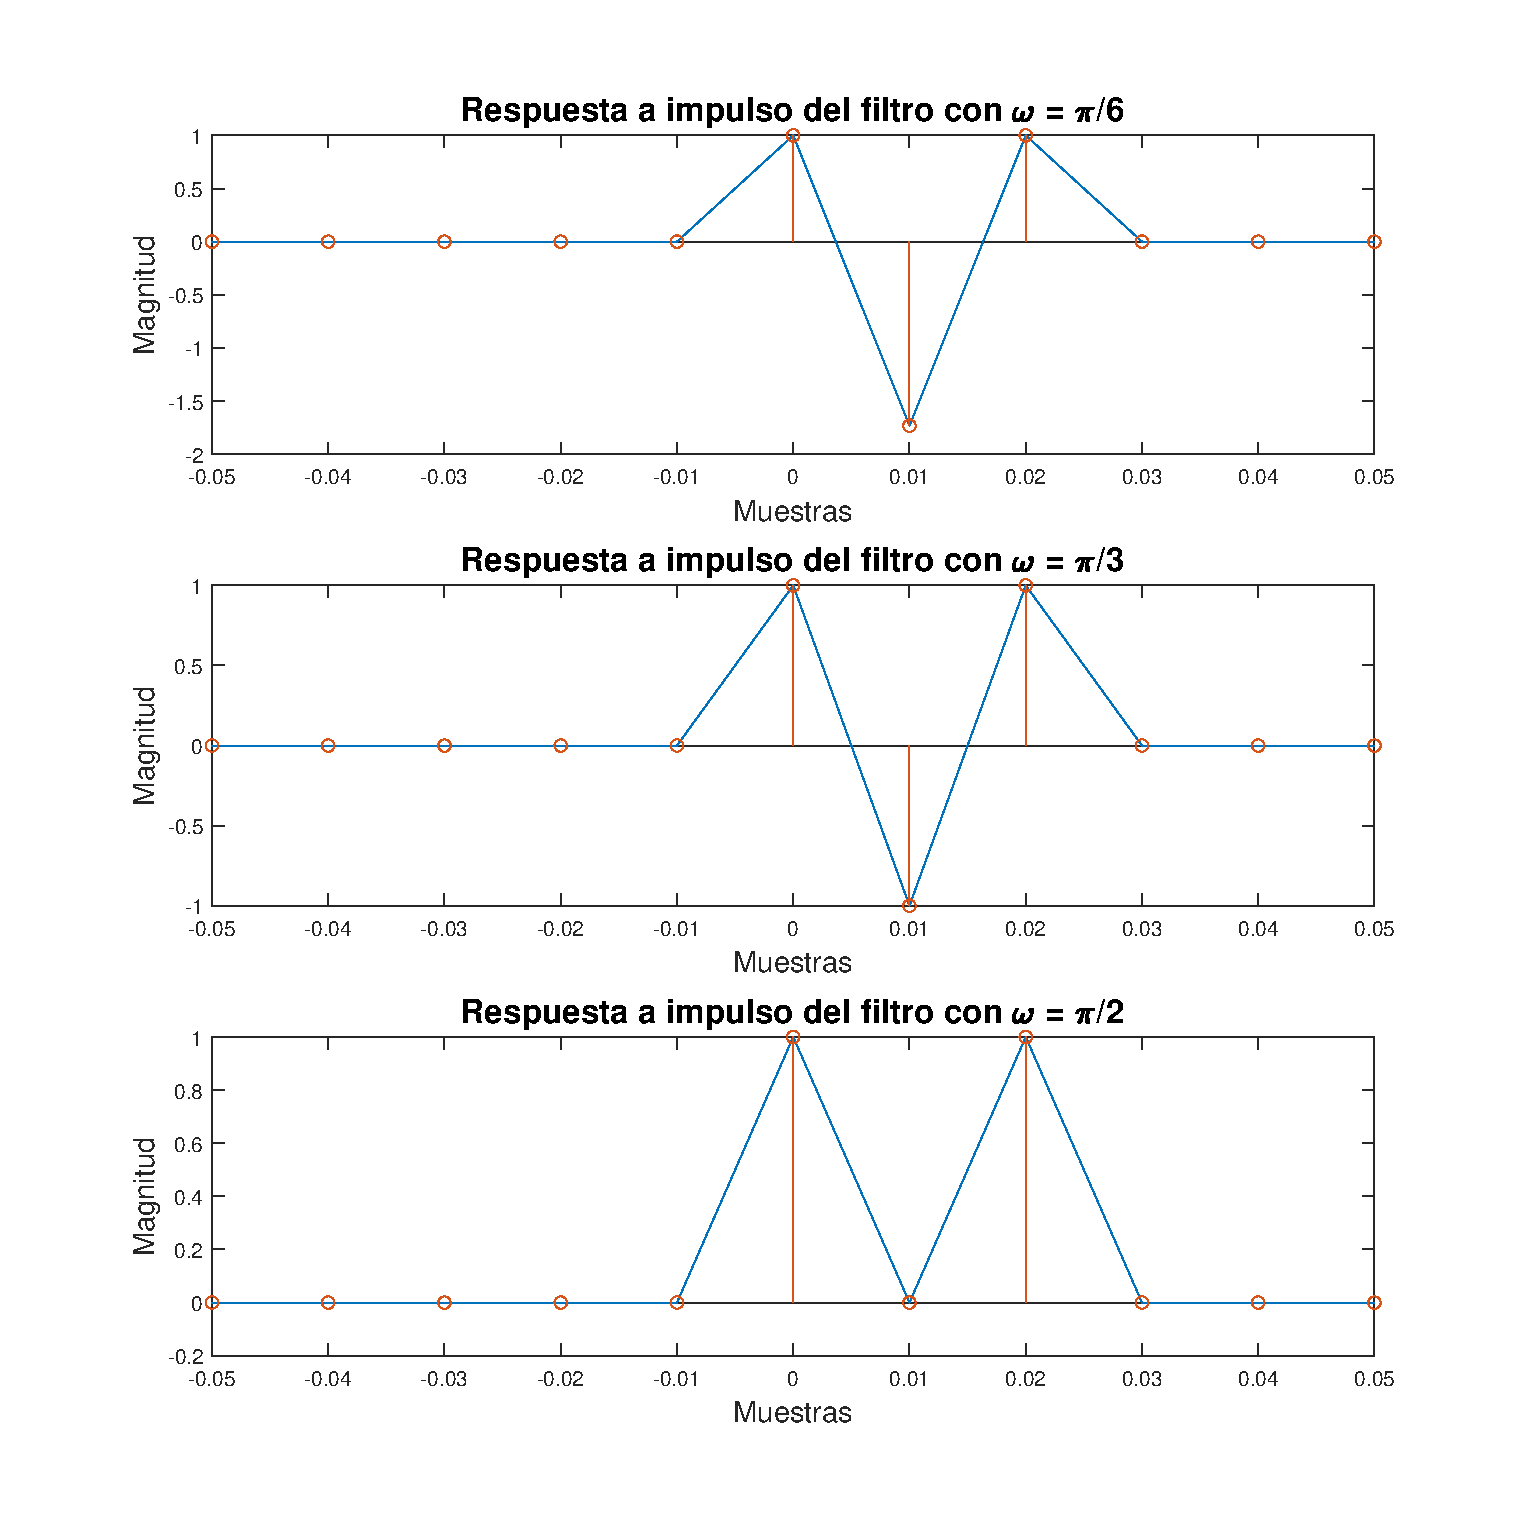
\includegraphics[scale = 0.5]{Figuras/p1_1-Respuesta_impulso.eps}
            \caption{Respuesta impulso del filtro para ángulos $ \theta = \left \lbrace \pi/6,~ \pi/3,~\pi/2 \right \rbrace$}
            \label{resp_impuilso}
        \end{figure}
    
    
    Haciendo el reemplazo de $z = e^{jwT_s}$ se puede obtener una expresión analítica para la función de transferencia del filtro diseñado en función de la frecuencia $\omega$.
    
        $$ H(z) = \frac{e^{2 j \omega T_s} - 2~e^{j \omega T_s}~cos(\theta)+ 1}{e^{2 j \omega T_s}}$$
    

    
    Se obtiene la respuesta en frecuencia del filtro diseñado  en función del ángulo para   $ \theta = \left \lbrace \pi/6,~ \pi/3,~\pi/2 \right \rbrace$   de donde tienen como resultado las gráficas de la figura \ref{frec_resp}
    
\begin{figure}[H]
    \centering
    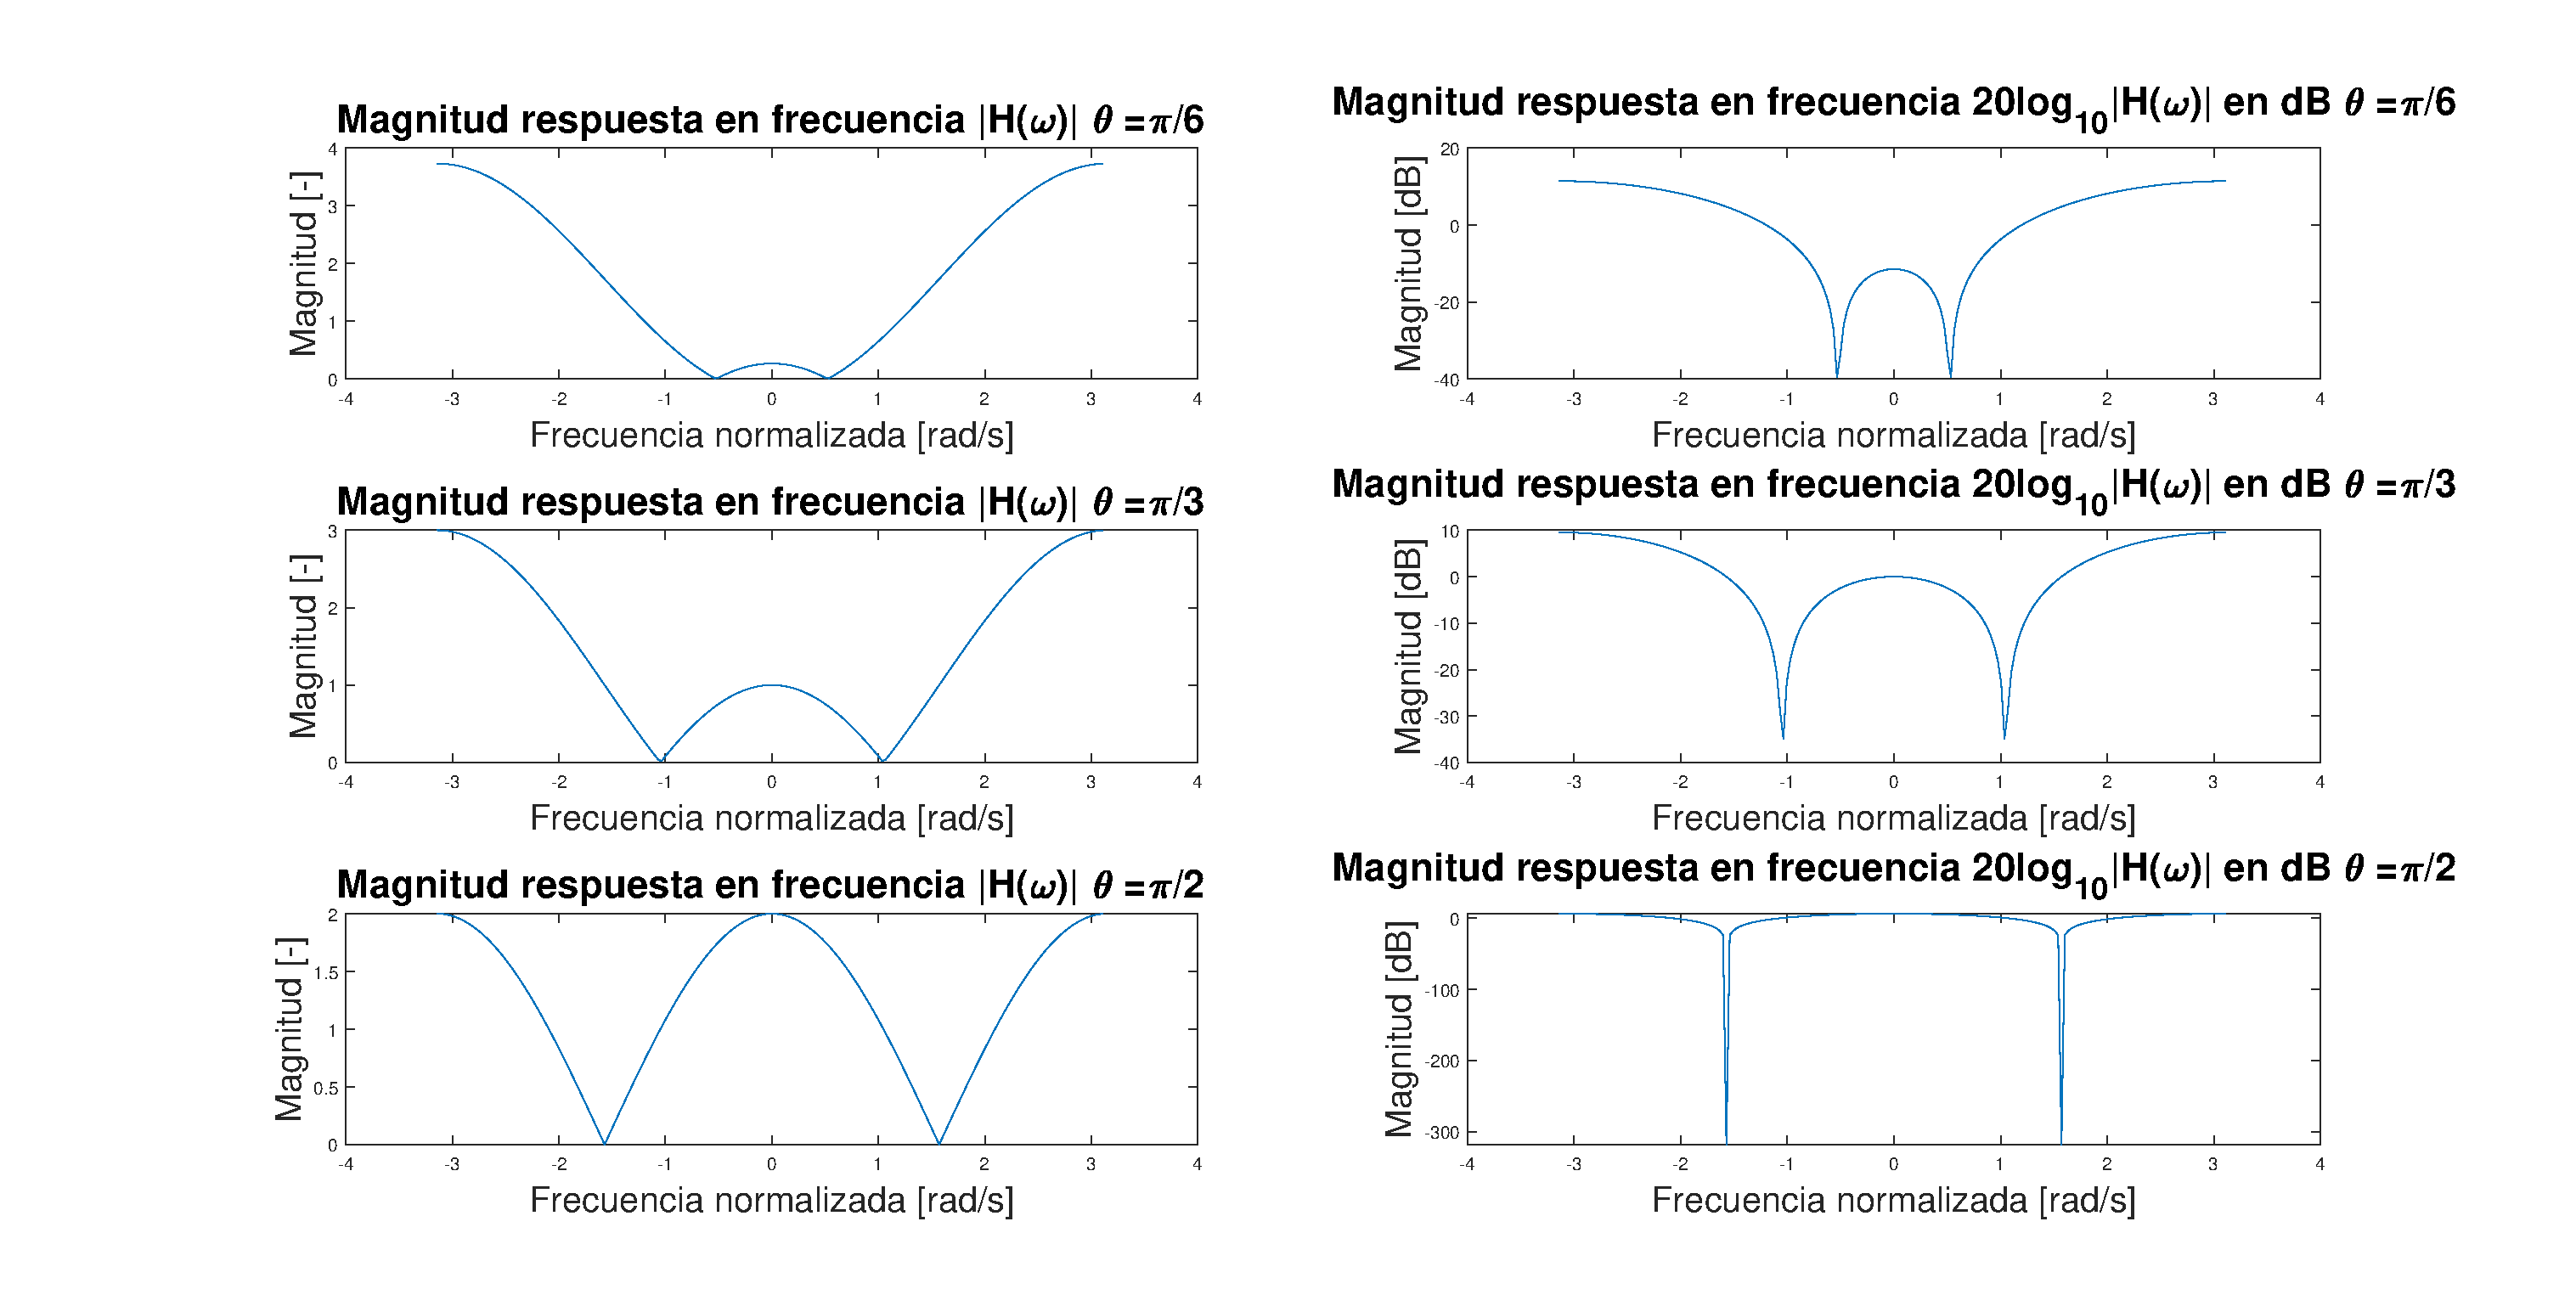
\includegraphics[scale = 0.3]{Figuras/p1_1-Respuesta_en_frecuencia.eps}
    \caption{Respuesta en frecuencia del filtro diseñado para  $ \theta = \left \lbrace \pi/6,~ \pi/3,~\pi/2 \right \rbrace$ }
    \label{frec_resp}
\end{figure}
    
    
    
    En la figura \ref{frec_superpuesta} se pueden observar las gráficas asociadas a los tres ángulos probados de manera superpuesta observar el efecto del ángulo en la respuesta en frecuencia del filtro.
    
    \begin{figure}[H]
        \centering
        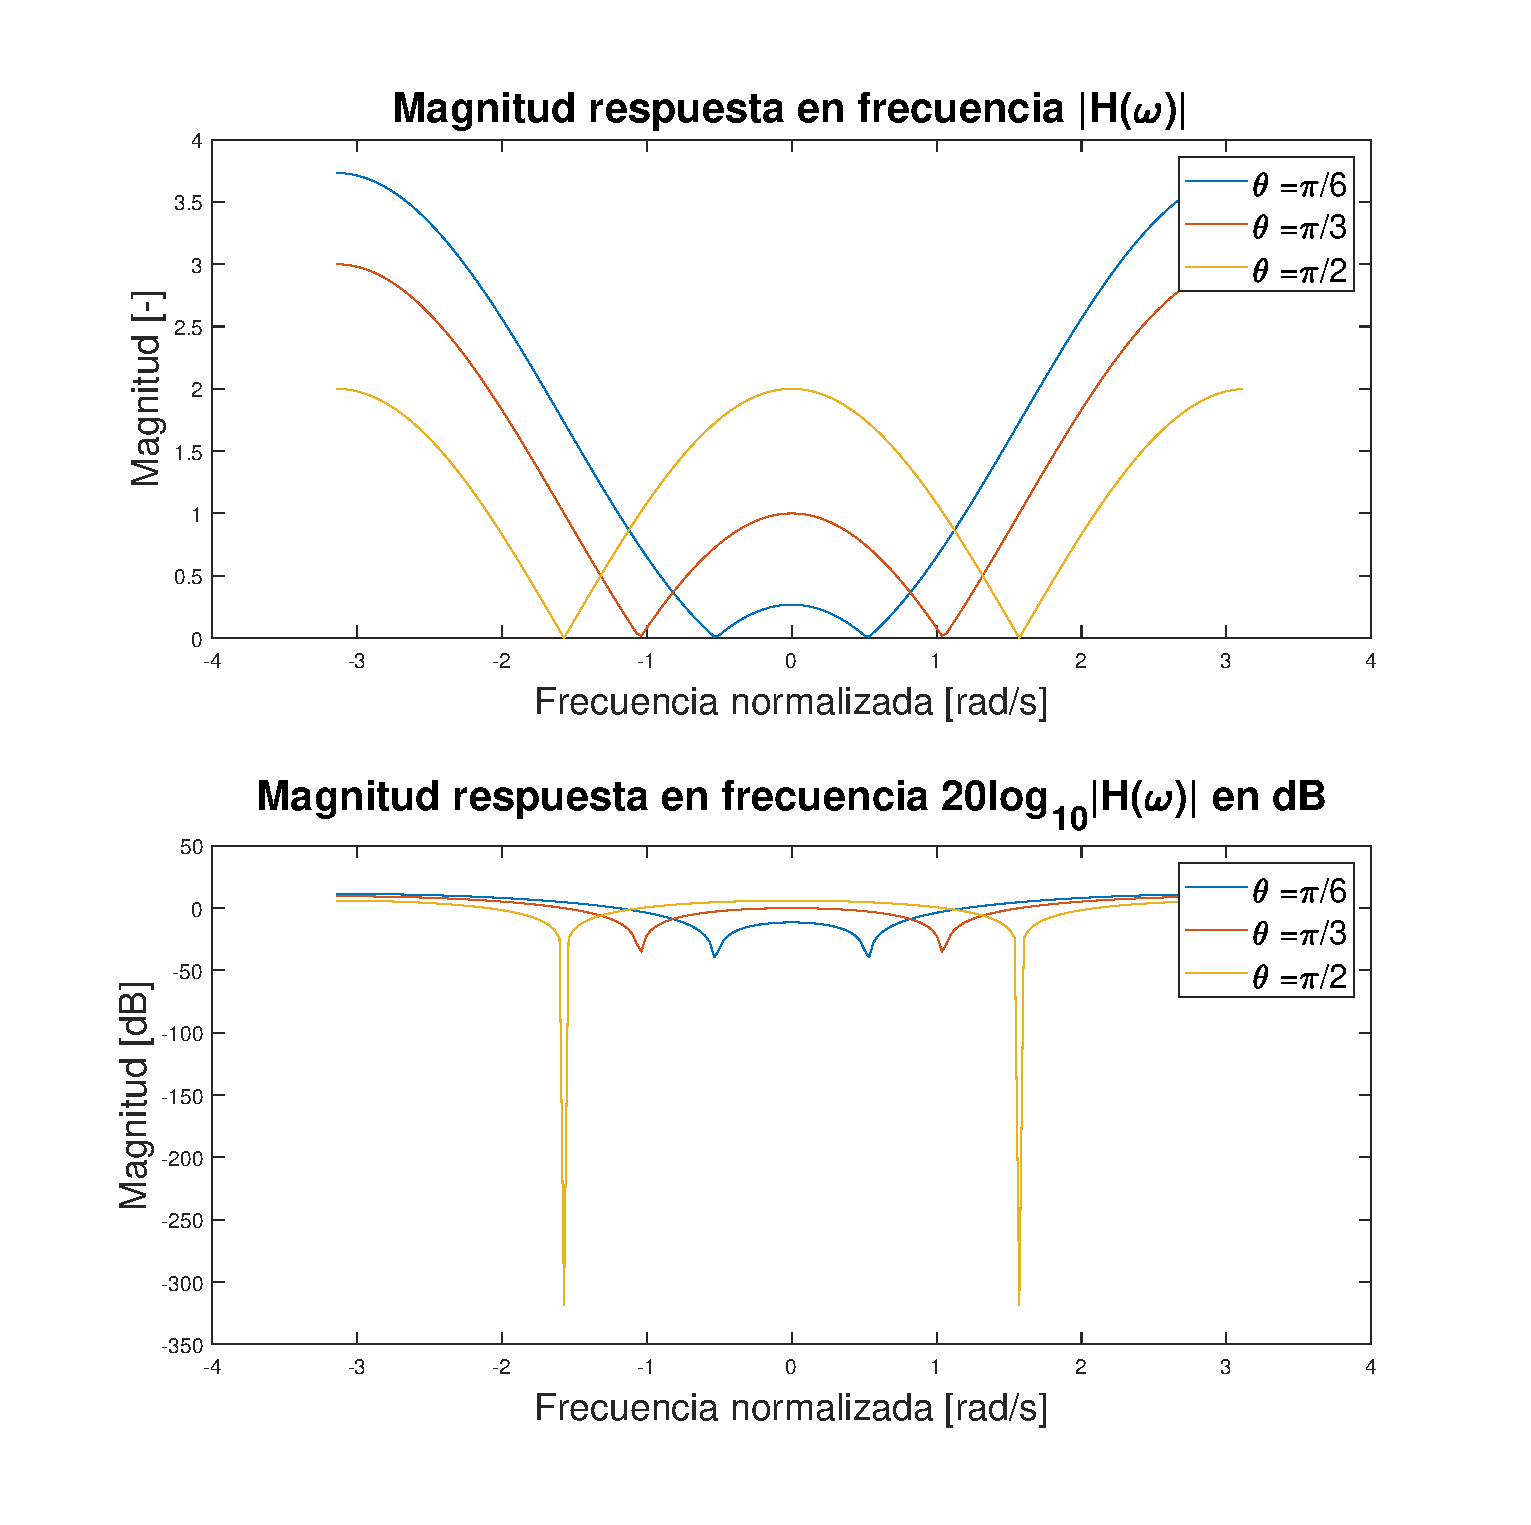
\includegraphics[scale = 0.4]{Figuras/p1_1-Respuesta_superpuesta.eps}
        \caption{Respuestas en frecuencia superpuestas del filtro diseñado para $ \theta = \left \lbrace \pi/6,~ \pi/3,~\pi/2 \right \rbrace$}
        \label{frec_superpuesta}
    \end{figure}
    


De las gráficas anteriores se puede ver como la frecuencia en la que la magnitud en frecuencia se hace cero, en una gráfica respecto a la frecuencia normalizada, corresponde justamente al valor de $\theta$, ya que para el conjunto de valores probados  $ \theta = \left \lbrace \pi/6,~ \pi/3,~\pi/2 \right \rbrace$, la respuesta en frecuencia del sistema se hace cero en $ rad/s = \left \lbrace 0.5235,~ 1.0471,~1.5707 \right \rbrace$

 
La relación que existe entre el ángulo $\theta$ con la respuesta en frecuencia del filtro con una frecuencia de muestreo $fs$ esta dada por 
$$ \theta = \frac{2 \pi f}{fs}$$ 

Ya que existe la razón directa entre $2\pi$ que corresponde a una vuelta completa al circulo unitario en el plano $\mathcal{Z}$ al igual que $fs$. Por lo que de esta forma se puede normalizar el valor de  una  frecuencia dada y llevarlo a la variable $\theta$. Observando el gráfico de la figura \ref{frec_superpuesta}, se puede concluir también que el valor de $f$ en la expresión anterior corresponde al valor de la frecuencia de corte del filtro en $Hz$ y por consiguiente $\theta$ es la frecuencia de corte del filtro frecuencia normalizada medida en $rad/muestra$.

%Rodrigo%%%%%%%%%%%%%%%%%%%%%%%%%%%%%%%%%%%%%%%%%%%%%%%%%%%%%%%%%%
\item  Se diseña un filtro que tiene dos polos conjugados dentro del círculo unitario en un ángulo $\theta$ en el plano $\mathcal{Z}$, con ganancia $1-r$. La función de transferencia queda dada por
\begin{align}
   H(z) &= \frac{1-r}{(z- re^{j \theta})(z-re^{-j \theta})} = \frac{1-r}{z^2 - 2zr\cos(\theta)+ r^2}\nonumber\\
   &= \frac{(1-r)z^{-2}}{1 - 2rz^{-1}\cos(\theta)+ r^2z^{-2}}\label{p1_2_Hz}
\end{align}
    
De donde se obtiene  la ecuación de diferencias: 
    
$$ y[n] = (1-r)x[n-2] +2r\cos(\theta )y[n-1] - r^2y[n-2]$$
    
Posteriormente se grafican las respuestas impulso a partir de la ecuación de recurrencia, para $r$ = 0.99, 0.9, 0.7 y $\theta = \pi/3$. Los gráficos se muestran en la figura \ref{fig:p1_2_ri}. Notar que el decaimiento de las respuesta a impulso es más lento a medida que $r$ está mas cercano al circulo unitario, pues se acerca a la zona inestable, y que el factor sinusoidal de las 3 respuestas a impulso comparten frecuencia. 

\begin{figure}[H]
    \centering
    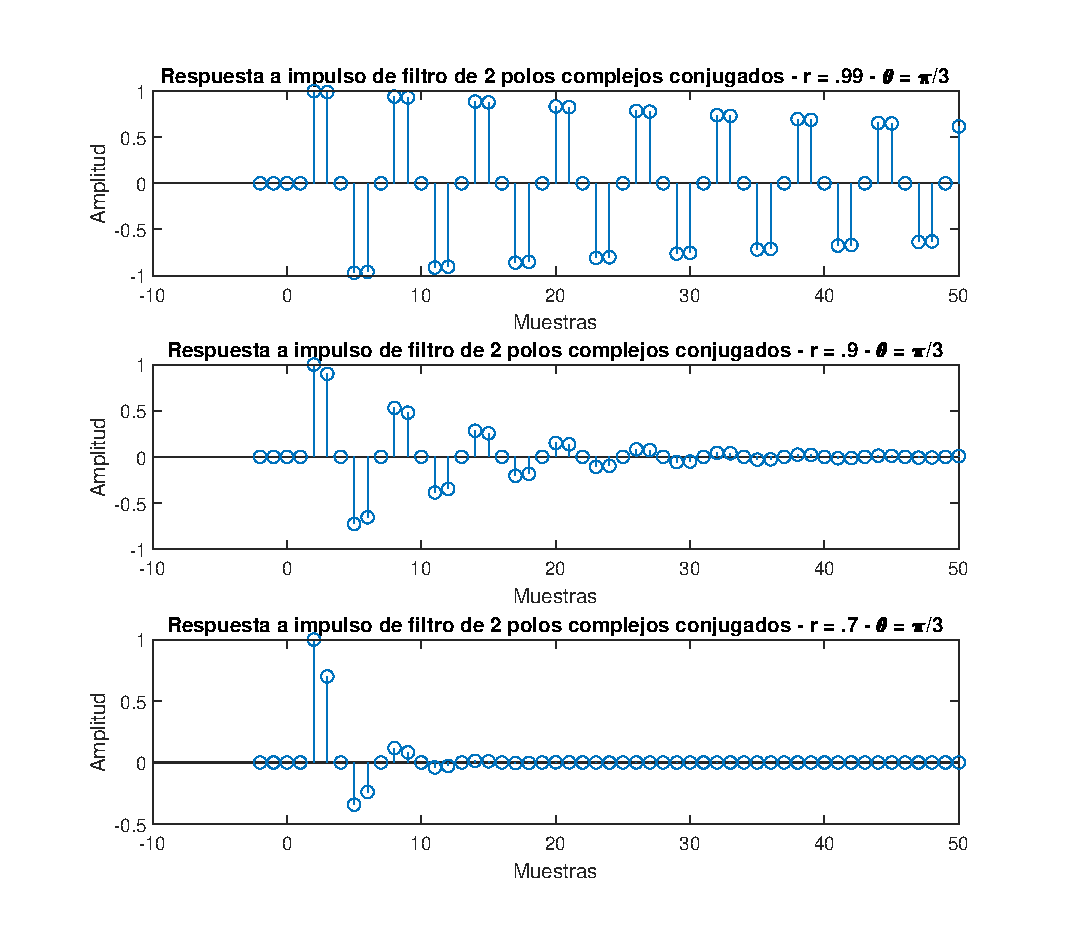
\includegraphics[width = .95\linewidth]{Figuras/p1_2_ri.eps}
    \caption{Respuestas a impulso de sistema de 2 polos complejos conjugados.}
    \label{fig:p1_2_ri}
\end{figure}

Luego, a partir de la función de transferencia (\ref{p1_2_Hz}) se obtiene la respuesta en frecuencia a partir de $H(z=e^{j\omega Ts})$, obteniendo:

$$ H(e^{j\omega Ts}) = \frac{1-r}{e^{2j\omega Ts} - 2ze^{j\omega Ts}\cos(\theta)+ r^2} $$

expresión que se usa para graficar las respuestas en frecuencia del filtro para $r$ = 0.99, 0.9, 0.7 y $\theta = \pi/3$. Las respuestas en frecuencia se muestran en la figura  \ref{fig:p1_2_rf}.

Notar que:
\begin{itemize}
    \item La frecuencia de resonancia se mantiene en $\theta = \tfrac{\pi}{3}$ para los 3 filtros.
    \item El peak es mayor a medida que $r$ a 1 , es decir, cuando los polos se acercan a la zona inestable.
    \item El filtro corresponde a un pasa banda el cual es mas selectivo (disminuye ancho de banda) a medida que $r$ crece
\end{itemize}

\begin{figure}[H]
    \centering
    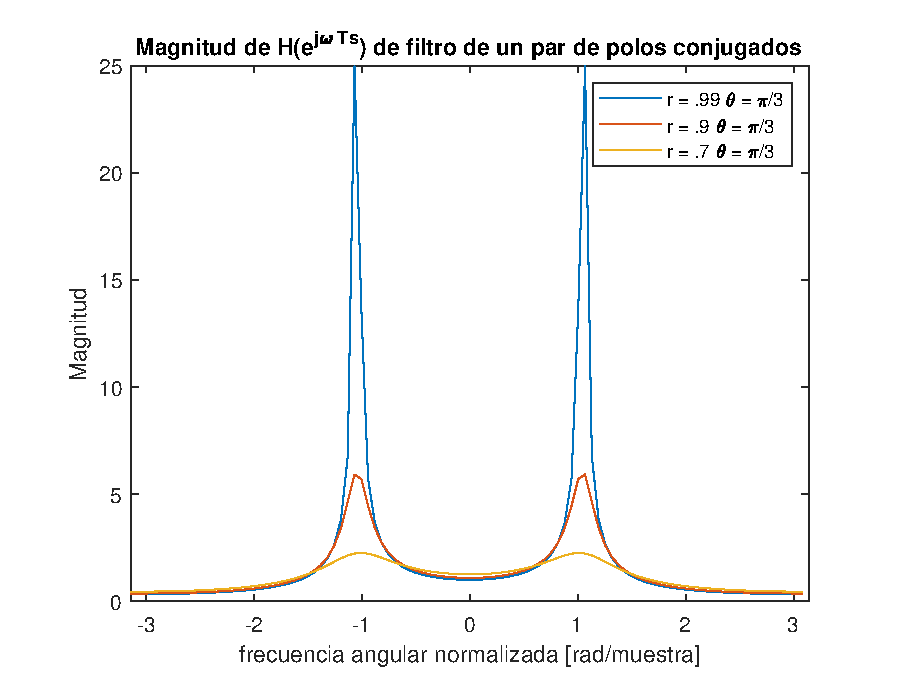
\includegraphics[width = .95\linewidth]{Figuras/p1_2_rf.eps}
    \caption{Respuestas en frecuencia de sistema de 2 polos complejos conjugados.}
    \label{fig:p1_2_rf}
\end{figure}
    
    

%%%%%%%%%%%%%%%%%%%%%%%%%%%%%%%%%%%%%%%%%%%%%%%%%%%%%%%%%%%%%%%%%%%
\item  Haciendo uso de la función  \texttt{DTFT.m} entregada en los recursos para el laboratorio se puede obtener el espectro en frecuencias correspondiente al archivo \texttt{nspeech.mat}, y identificar la frecuencia del tono puro presente en el archivo, como se ve en la figura \ref{nspeech_tone}

\begin{figure}[H]
    \centering
    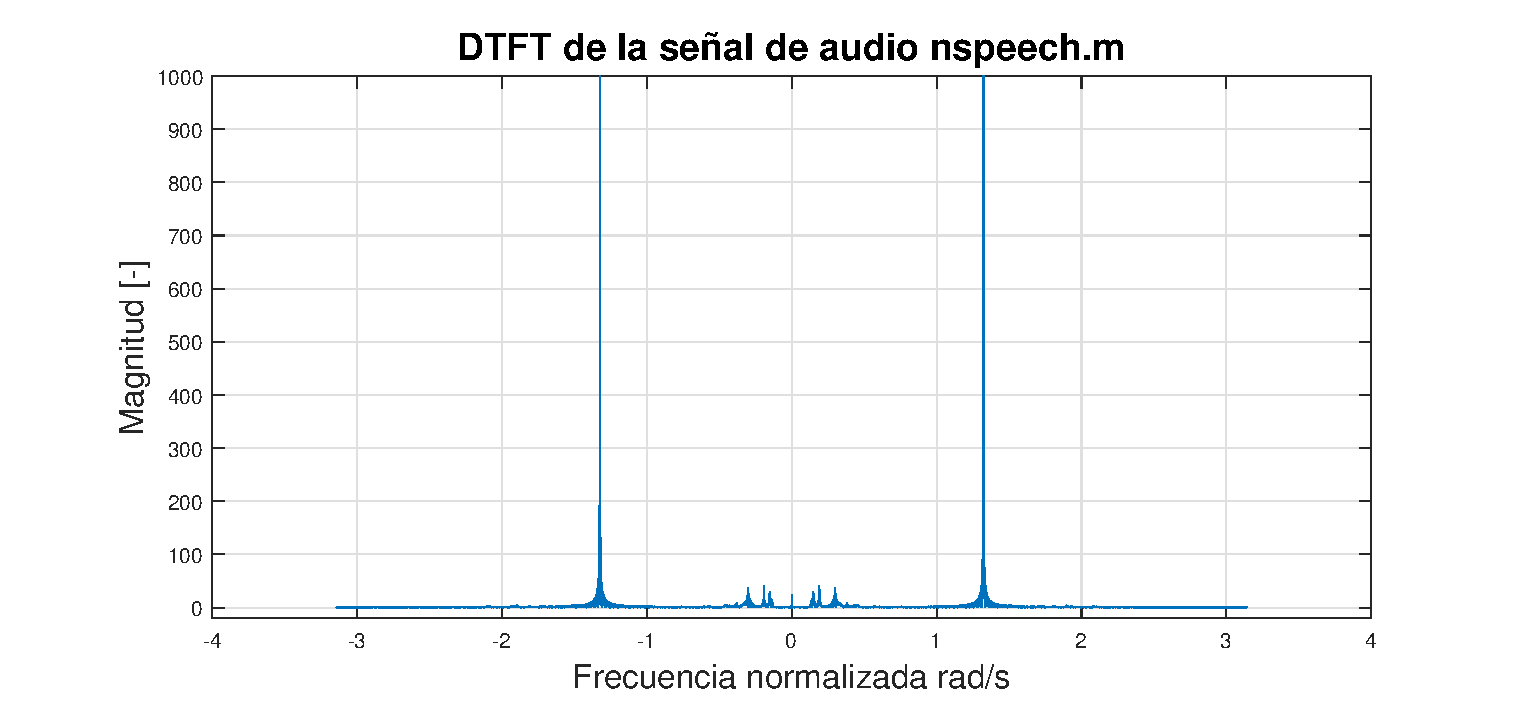
\includegraphics[scale = 0.6]{Figuras/p1_3-DTFT.eps}
    \caption{Espectro en frecuencia normalizada de \texttt{nspeech.mat}}
    \label{nspeech_tone}
\end{figure}

\end{enumerate}

Donde se puede ver que el tono se encuentra en la frecuencia 1.323. Como la gráfica está en frecuencia normalizada, este valor corresponde al ángulo $\theta = 1.323$;

Luego se puede diseñar un filtro FIR que rechace esta frecuencia mediante dos ceros conjugados en esta frecuencia $\theta$

$$ H(z) = (z-e^{j\theta})(z - e^{-j\theta})  = z^2 - 0.49 + 1$$

Por lo que los coeficientes $b_k$ del filtro serían

$$B = [1 ~-0.49 ~~1]$$


Al implementar el filtro FIR mediante convolución, y aplicar el filtrado a la señal se obtienen los resultados presentes en las gráficas de la figura \ref{Fir}

\begin{figure}[H]
    \centering
    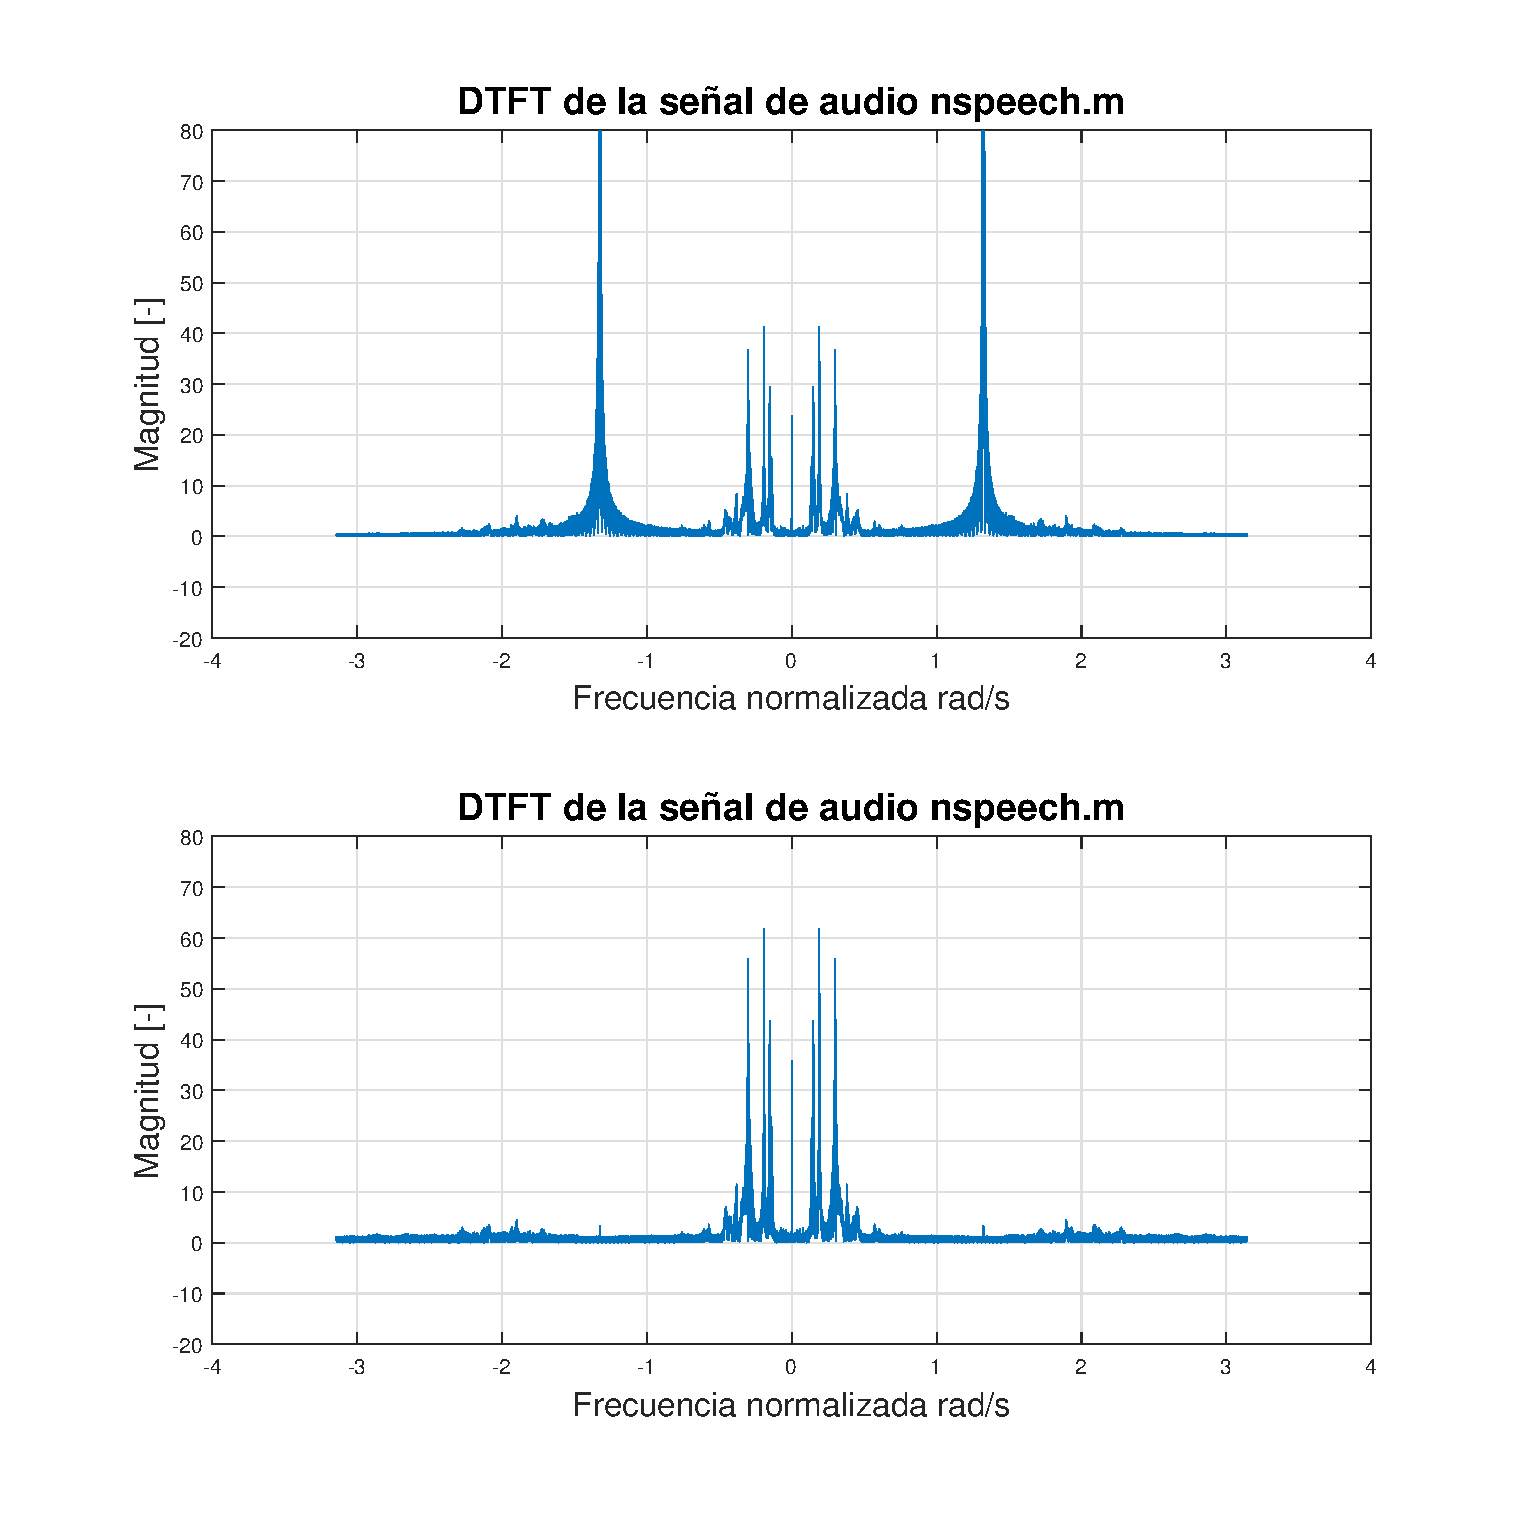
\includegraphics[scale = 0.4]{Figuras/p1_3-nspeech_filtrada.eps}
    \caption{Espectro en frecuencia del archivo \texttt{nspeech.mat} antes y después de ser filtrado.}
    \label{Fir}
\end{figure}

En donde se puede ver claramente que el tono puro que se encontraba en el archivo original se encuentra visualmente imperceptible luego de aplicar el filtro.

Cabe mencionar que el archivo original correspondía a un vector que contenía 13061 muestras, pero el resultado obtenido al aplicar la convolución con el filtro diseñado corresponde a un arreglo con tamaño distinto al original. Esto se debe a que para aplicar el comando de convolución \texttt{conv(u,v)} por lo que el tamaño del vector obtenido corresponde a $ \texttt{length(u)} + \texttt{length(b)} -1$ basado en  cómo se desarrolla el proceso de convolución.



\item Se busca filtrar el ruido presente en el archivo \texttt{pcm.mat} para lo que se diseña un filtro de tipo IIR. Se grafica el espectro en frecuencia de el archivo de audio para poder identificar cual es la frecuencia que contiene la  información que se desea conservar, esto se muestra en la gráfica de la figura \ref{dtft_pcm}

\begin{figure}[H]
    \centering
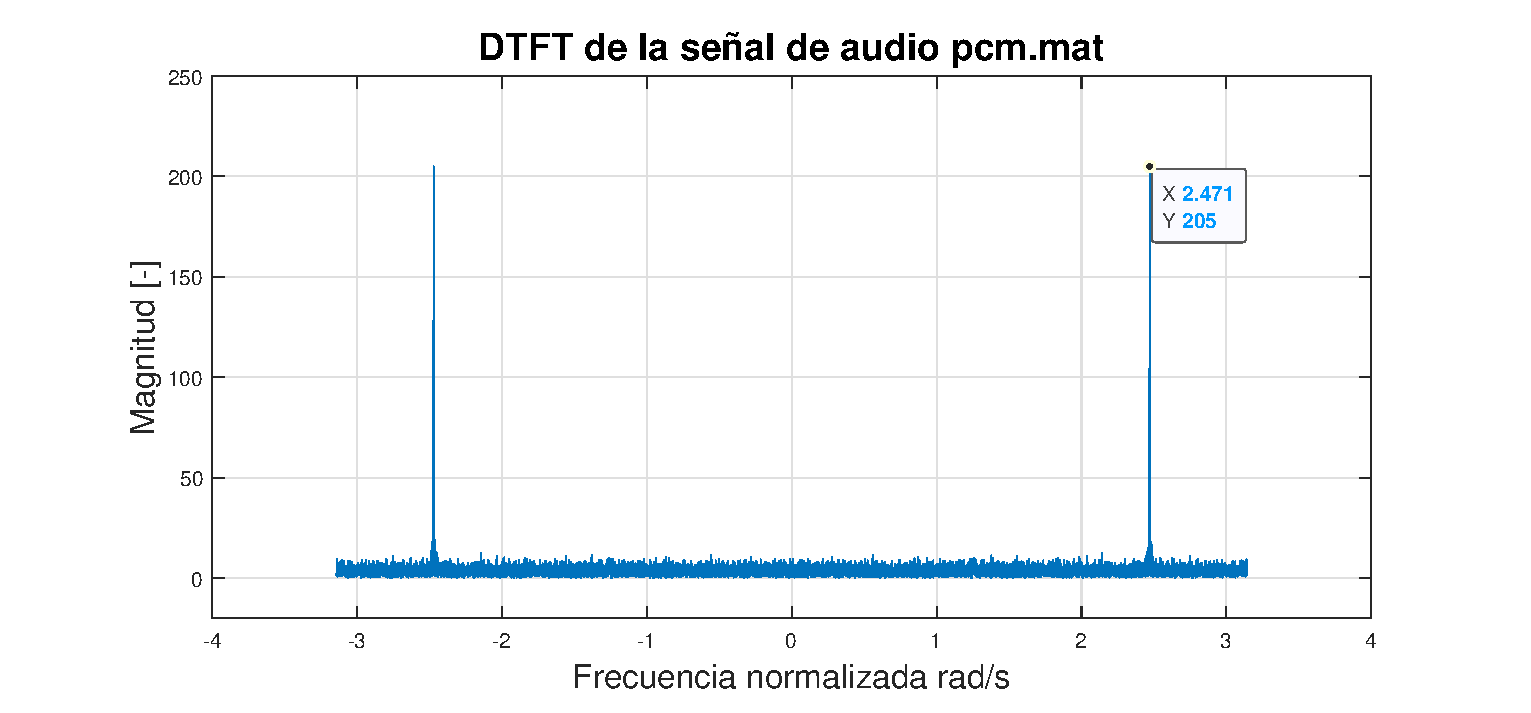
\includegraphics[scale = 0.6]{Figuras/p1_4-DTFT_pcm.eps}
    \caption{Espectro en frecuencia normalizada de \texttt{pcm.mat}.}
    \label{dtft_pcm}
\end{figure}

Donde se puede ver que el tono se encuentra en la frecuencia 1.323. Como la gráfica está en frecuencia normalizada, este valor corresponde al ángulo $\theta = 2.471$;


Se diseña entonces un filtro IIR con $r = 0.99$ y $\theta = 2.471$,  con función de transferencia

$$  H(z) = \frac{(1-r)z^2}{(z-re^{j\theta})(z-re^{-j\theta})} = \frac{(1-r)z^2}{z^2 -2~z~cos(\theta) + r^2}$$

Con coeficientes $a_k$

$$ a_k = [1 ~~-2cos(\theta) ~~ r^2]$$




Al implementar el filtro IIR mediante recurrencia, y aplicar el filtrado a la señal se obtienen los resultados presentes en las gráficas de la figura \ref{IIR}

\begin{figure}[H]
    \centering
    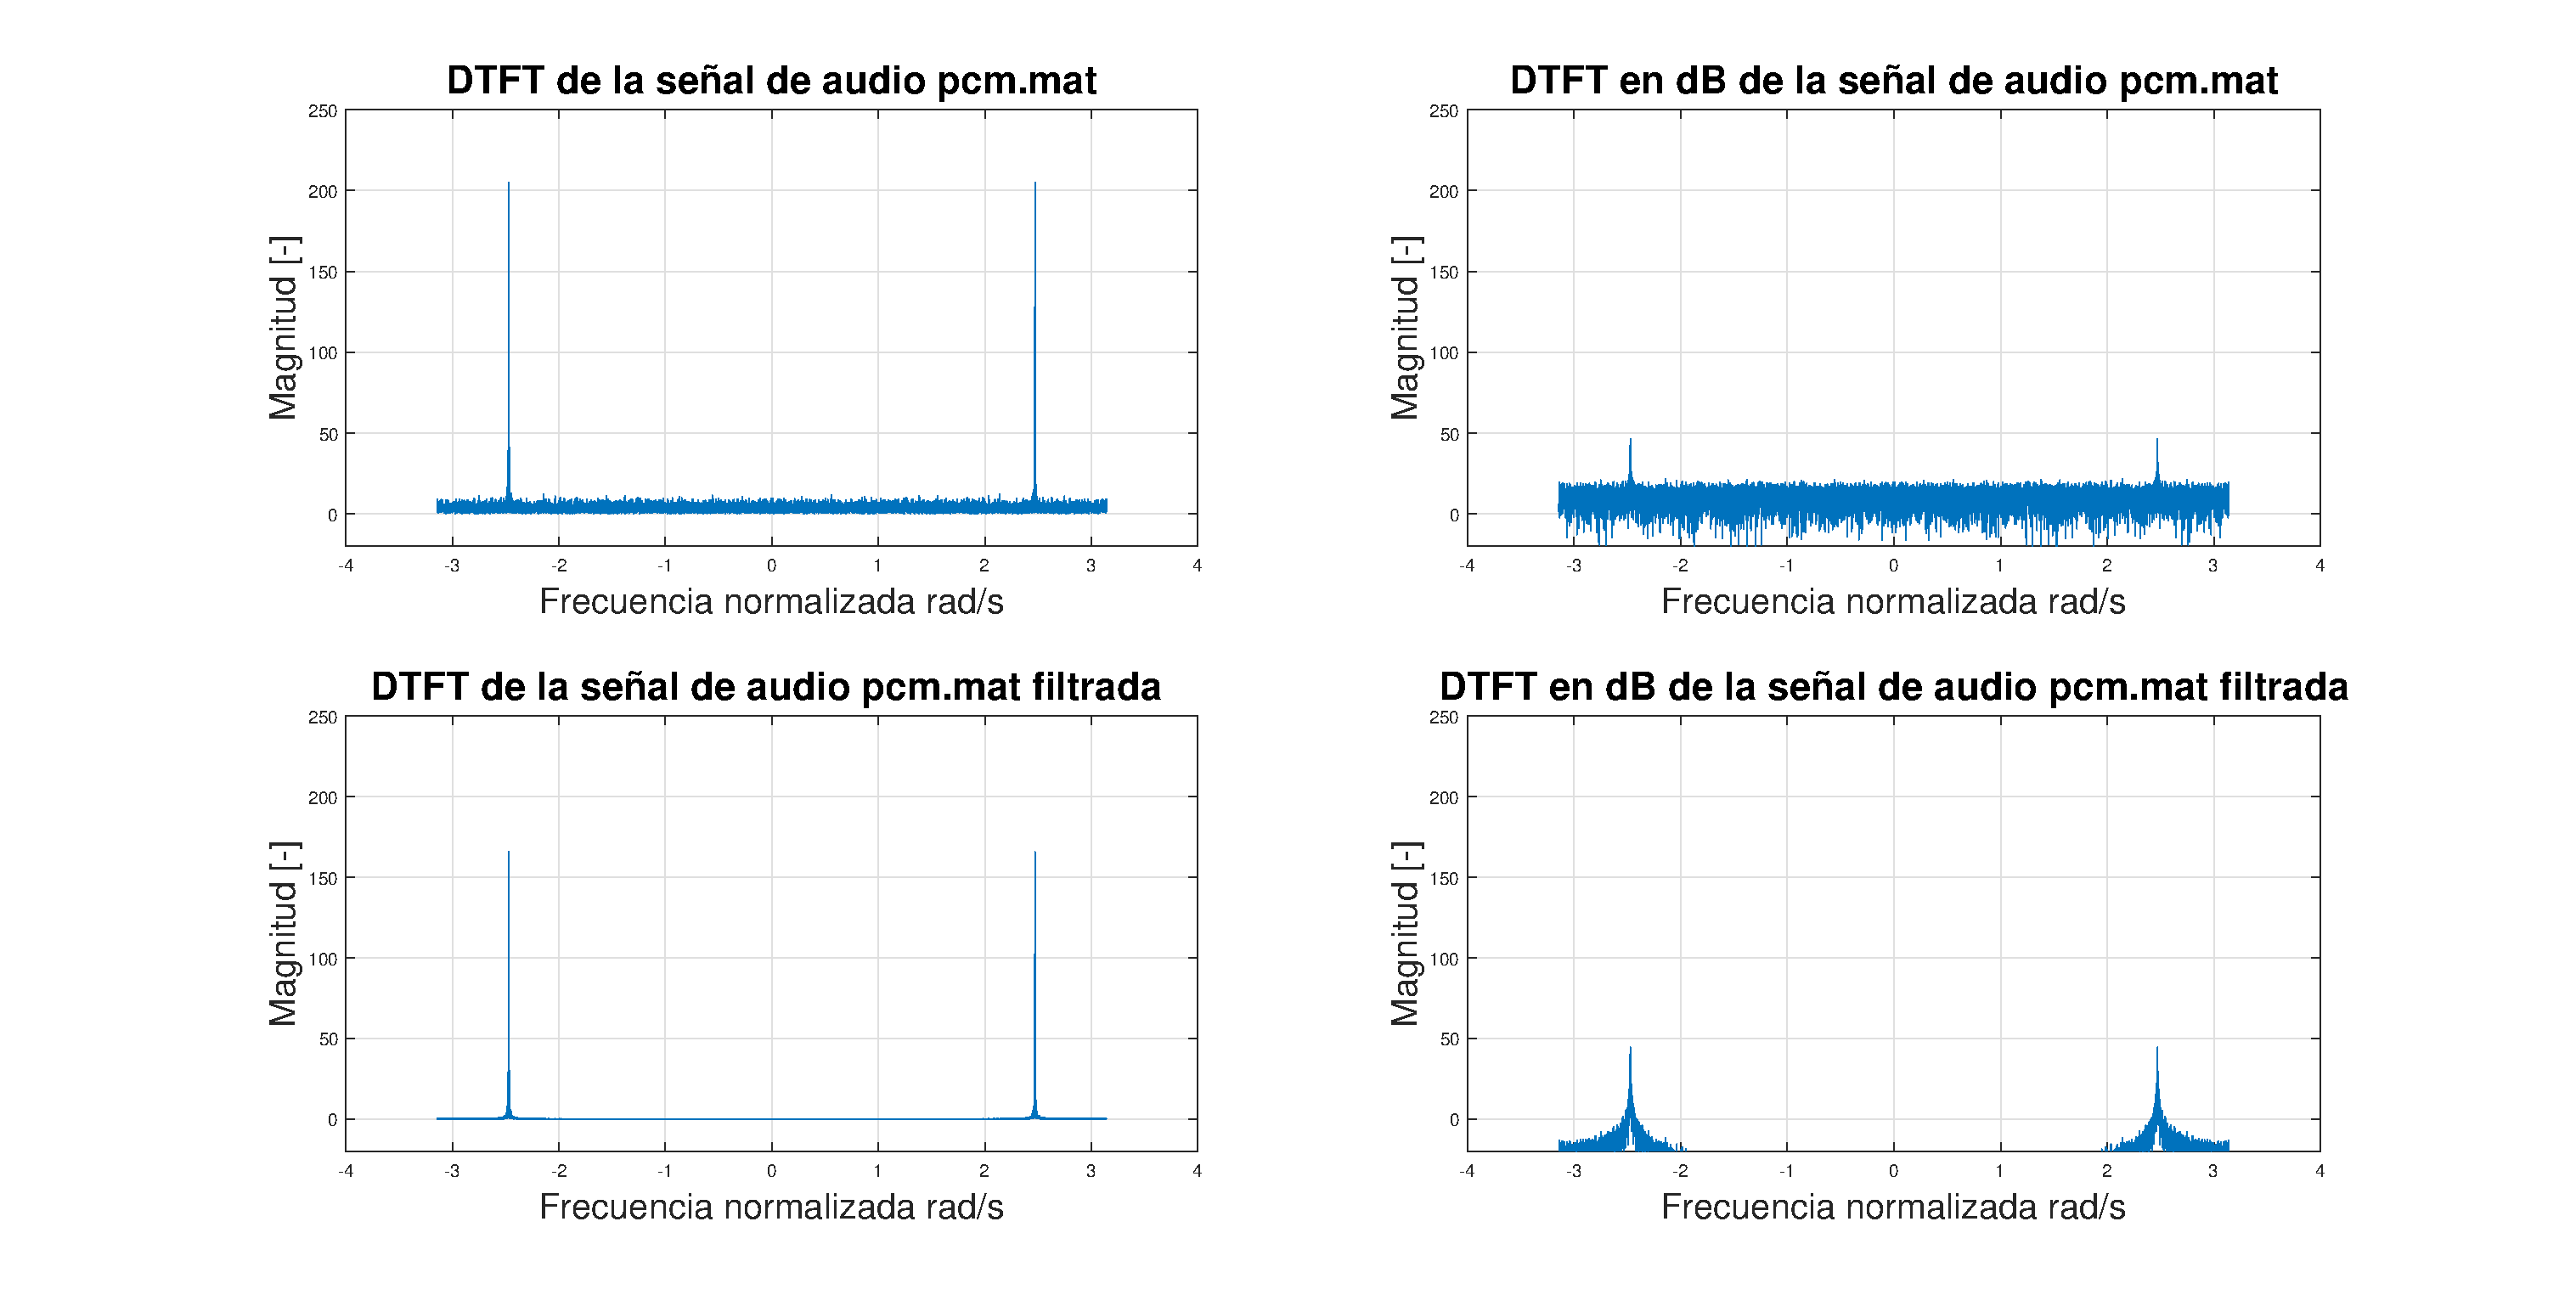
\includegraphics[scale = 0.3]{Figuras/p1_4-pcm_filtrada.eps}
    \caption{Espectro en frecuencia del archivo \texttt{pcm.mat} antes y después de ser filtrado.}
    \label{IIR}
\end{figure}


En la figura anterior se puede observar tanto en magnitud como en decibeles cómo se ha eliminado de forma significativa  el ruido presente en el archivo original.




\clearpage

\section{Diseño de filtros FIR usando ventanas}
\begin{enumerate}
    \item Se estudia la aproximación a un filtro pasa bajos mediante al truncamiento de la respuesta a impulso haciendo uso  de una ventana rectangular  con el filtro dado por 
    
 $$   
h[n]= \left\{ \begin{array}{lcc}
             \frac{w_c}{pi}~sinc(\frac{w_c}~{\pi} (n- \frac{N-1}{2})) &   ,  & n = 0,1,..., N-1 \\
             \\ 0 &  ,  & e.o.c \\
  
             \end{array}
   \right.  
   $$


Donde $\omegaw_c$ corresponde a la frecuencia de corte del filtro, en este caso este parámetro tomará el valor de $\frac{2\pi}{3}$

Se crean tres filtros con $N = 21,~ 101,~ 1001$, para los cuales se obtuvieron las siguientes gráficas para la magnitud  y fase de su respuesta en frecuencia utilizando la función \texttt{DTFT.mat}.

\begin{figure}[H]
    \centering
    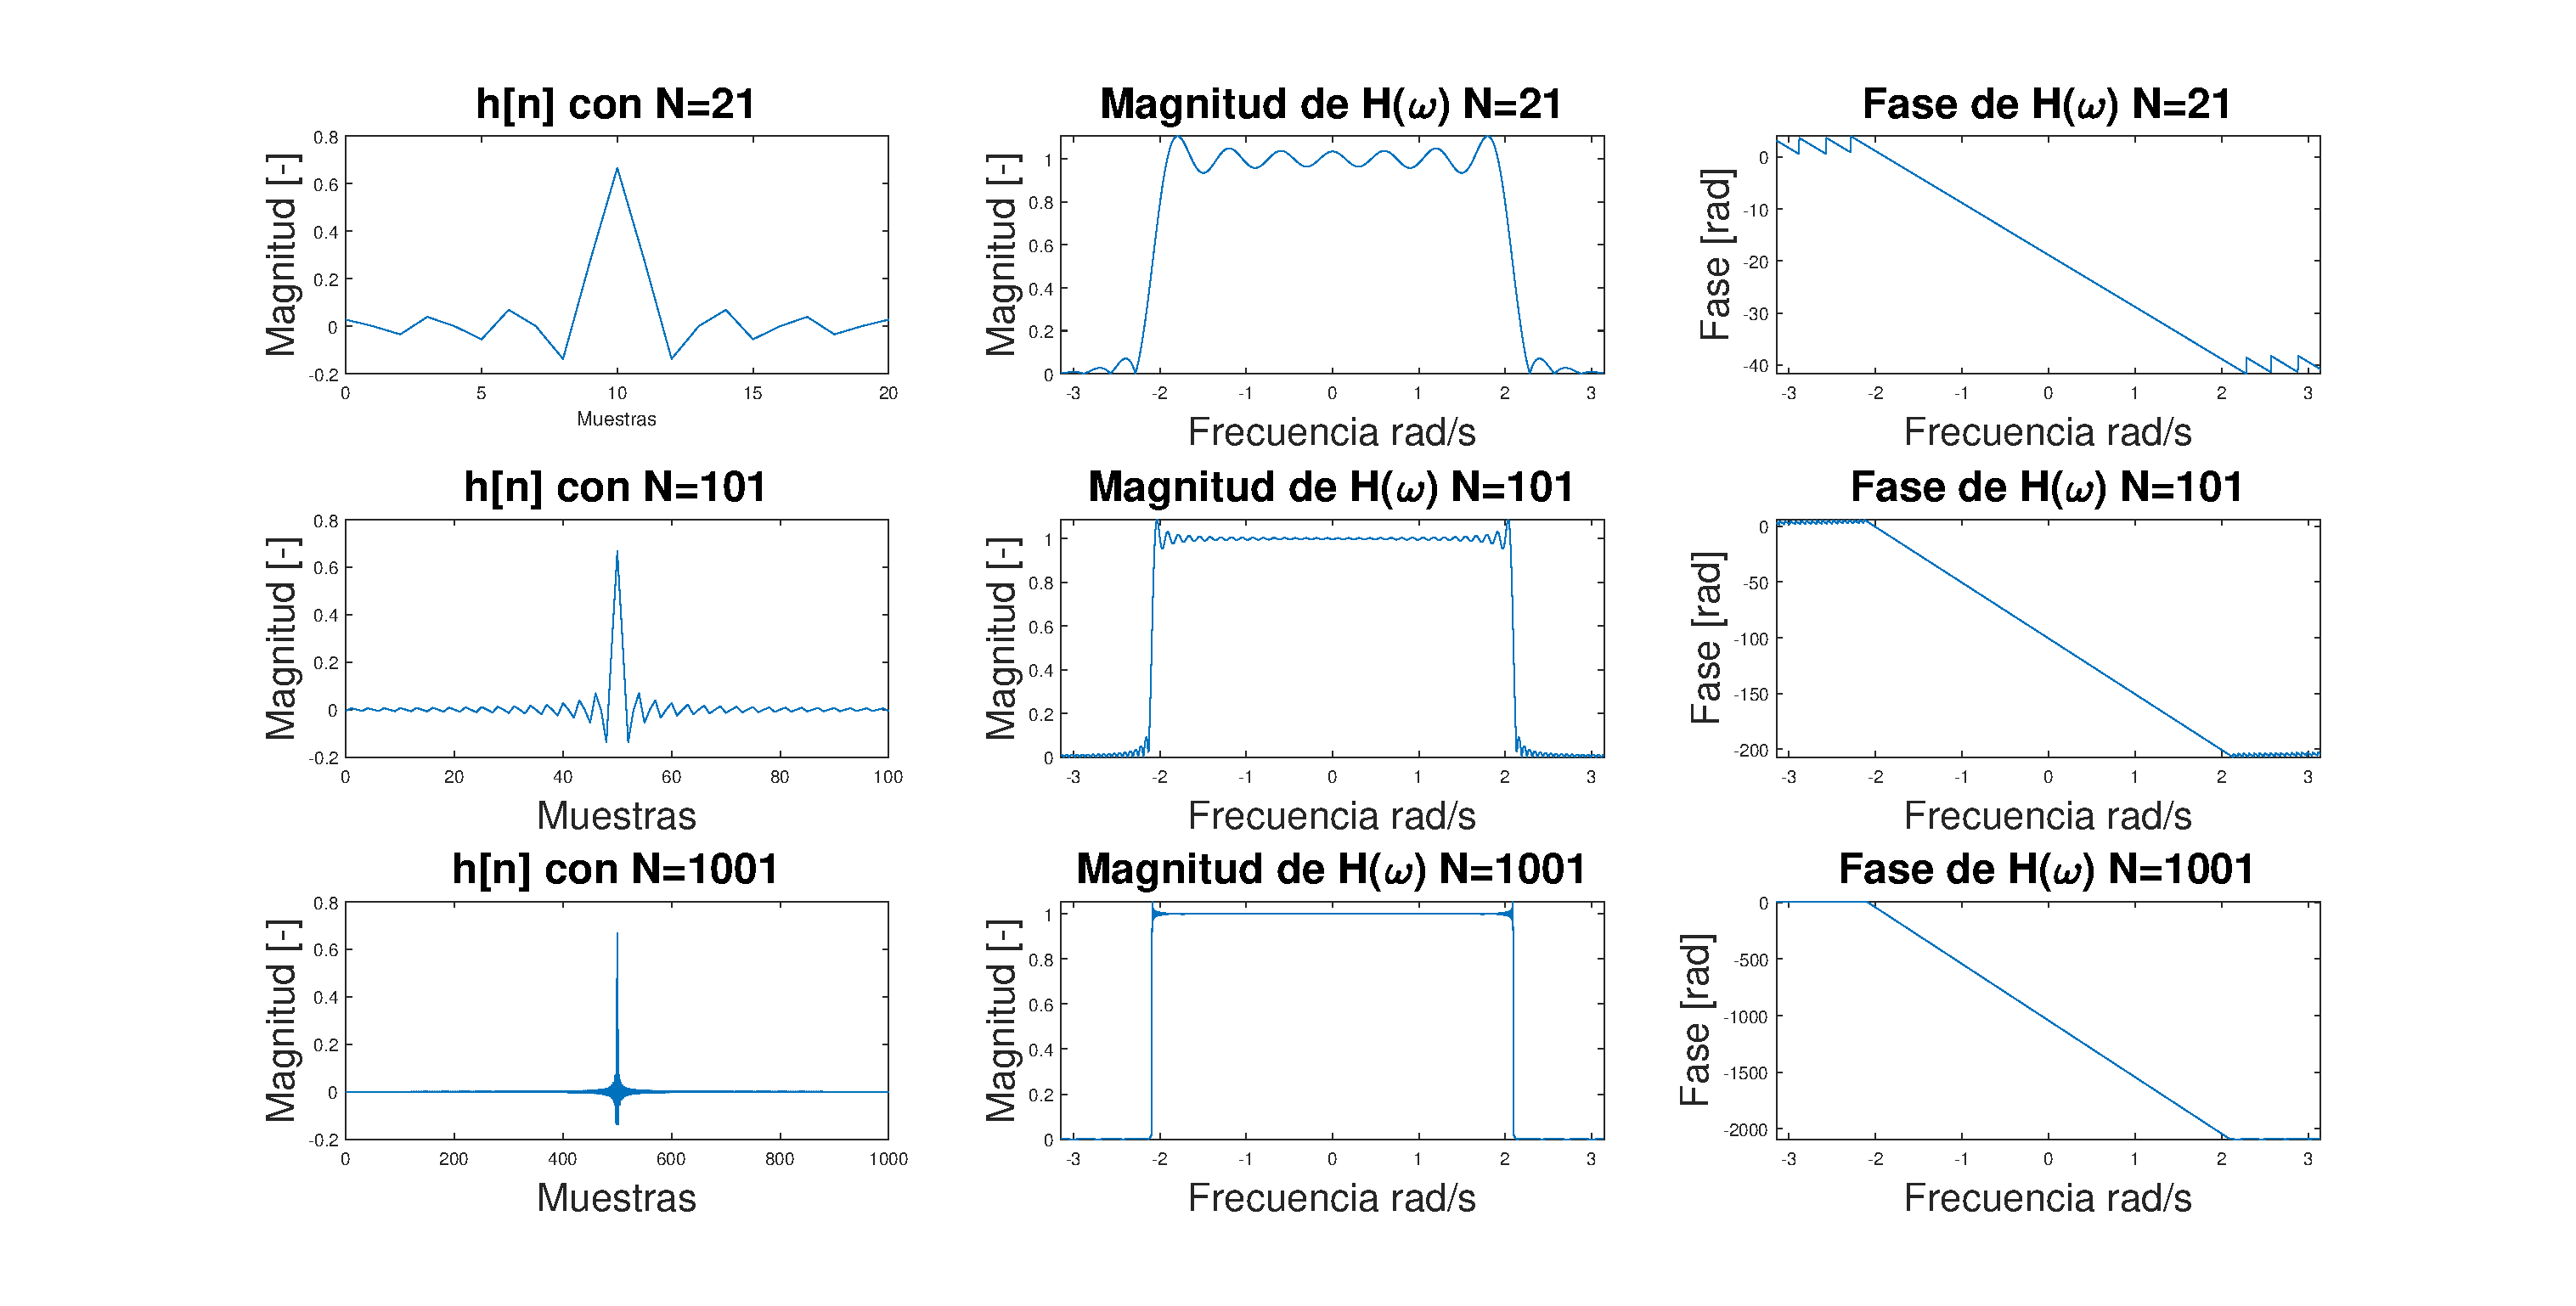
\includegraphics[scale = 0.3]{Figuras/p2_1-Sincs.eps}
    \caption{Magnitud y fase de la respuesta en frecuencia para los filtros de ventana rectangular con  con $N = 21,~ 101,~ 1001$}
    \label{}
\end{figure}

Se puede observar que, como era de esperarse, una ventana con un valor de N mayor genera una respuesta en frecuencia más prolija, con menos ripple y con pendientes más pronunciadas en las frecuencias de corte acercándose de esta forma a el comportamiento de un filtro ideal, al utilizar un valor de N menor la respuesta en frecuencia se puede distorsionar debido a la presencia clara de ripple y la atenuación de las frecuencias posteriores a la frecuencia de corte no es tan efectiva.

Lo mismo ocurre con la fase, mientras más elevado es el valor de N para el filtro, la respuesta en la fase se vuelve más plana en las frecuencias que superan en magnitud a la frecuencia de corte del filtro, mientras que las frecuencias que no se atenúan por el filtro para todos los valores de N evaluados se comportan de forma similar.



\item Para comparar las propiedades espectrales y temporales de los filtros FIR construidos se hace uso de las ventanas predefinidas por MATLAB:  \texttt{freqz}, \texttt{rectwin}, \texttt{hann}, \texttt{hamming},
\texttt{blackman}, y \texttt{bartlett}; que corresponden a las ventanas de tipo   rectangular, hamming, hanning, blackman, y bartlett respectivamente.  Esto utilizando $1 ~kps$ como tasa de muestreo de cada ventana y una duración de $100~ms$.

En la figura \ref{ventanas_tiempo} se puede observar el comportamiento en el tiempo para cada tipo de ventana.

\begin{figure}[H]
    \centering
    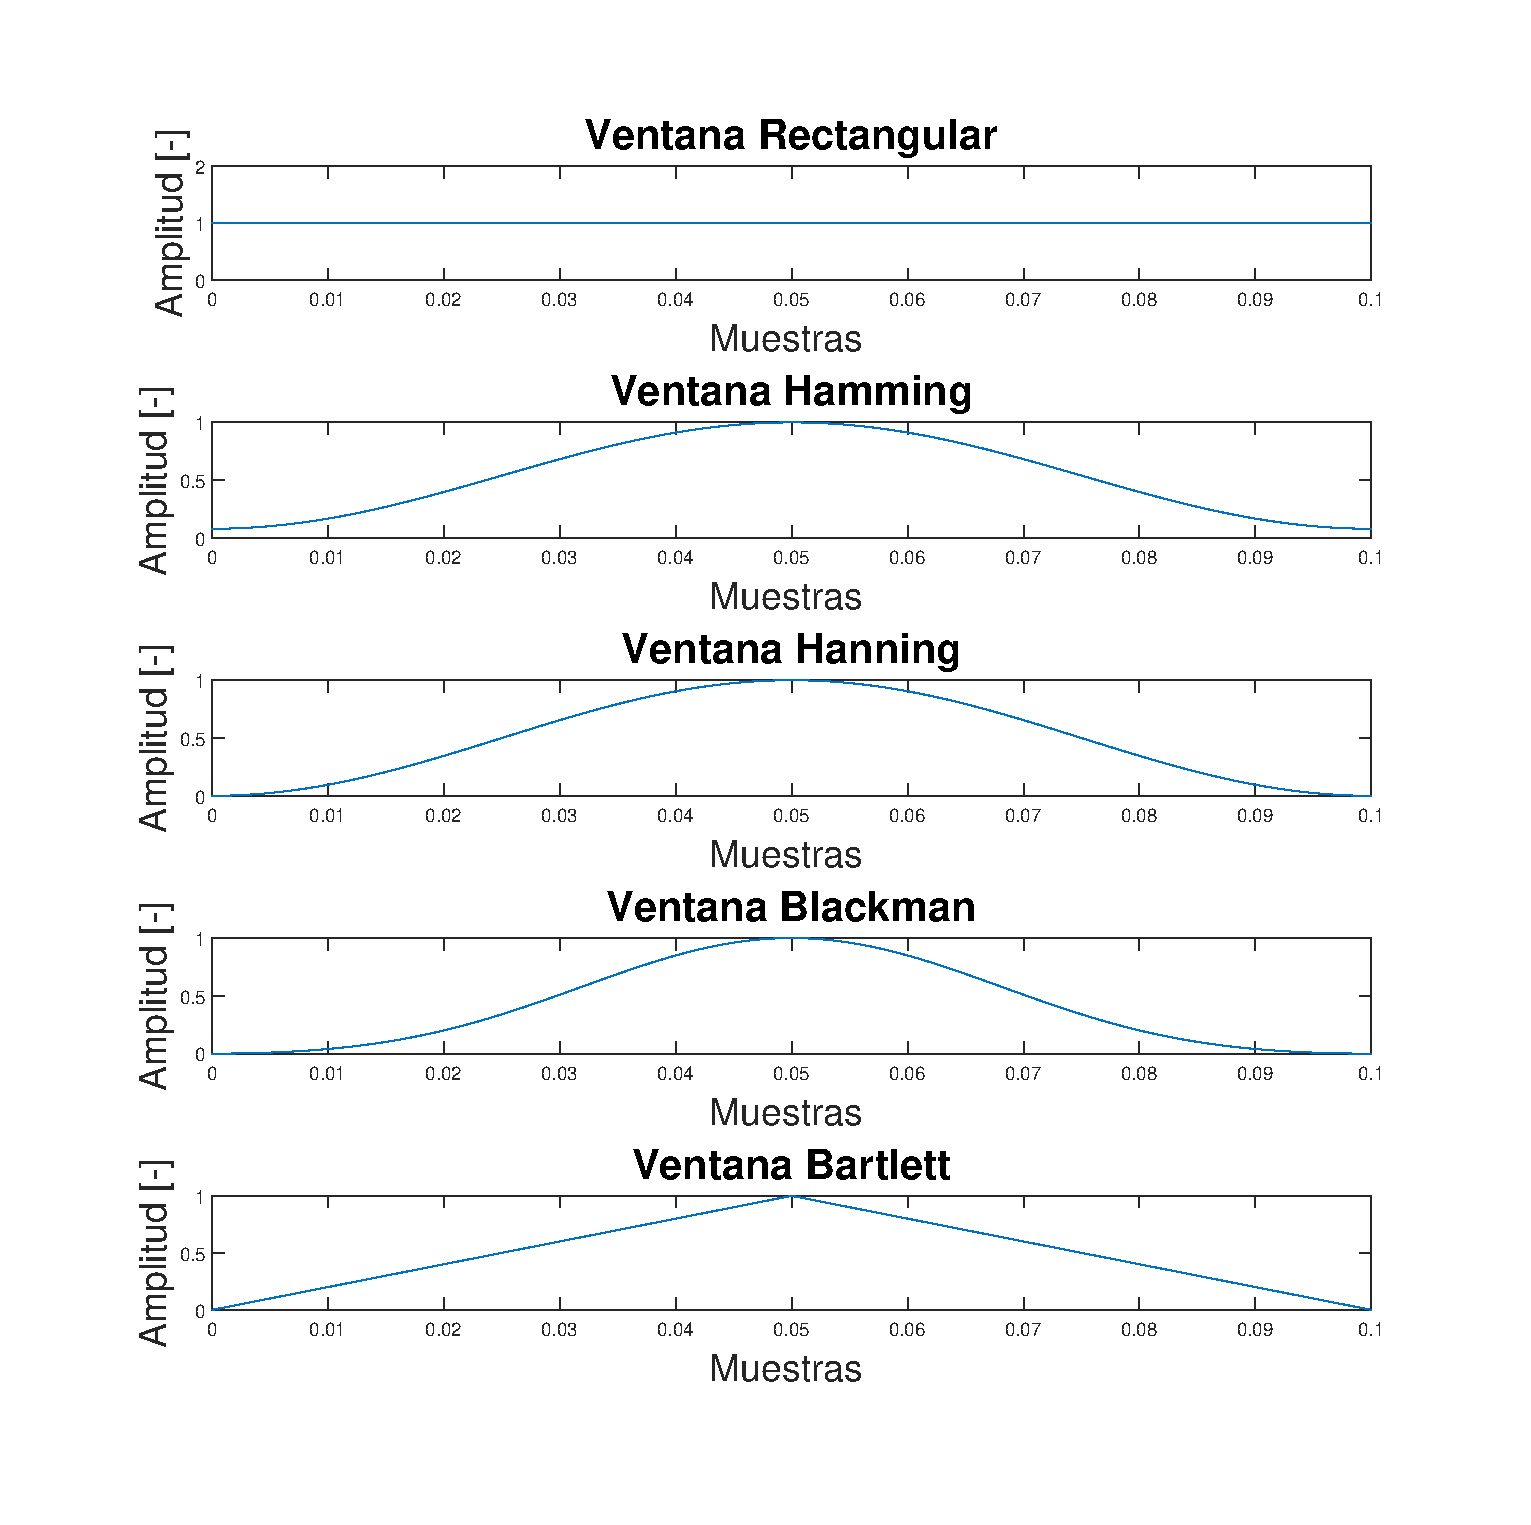
\includegraphics[scale = 0.5]{Figuras/p2_2-Ventanas-tiempo.eps}
    \caption{Ventanas rectangular, hamming, hanning, blackman, y bartlett en el tiempo.}
    \label{ventanas_tiempo}
\end{figure}


En la figura \ref{ventanas-magnitud} se puede ver cual es el comportamiento en  frecuencia de cada uno de los tipos de ventanas utilizadas.

\begin{figure}[H]
    \centering
    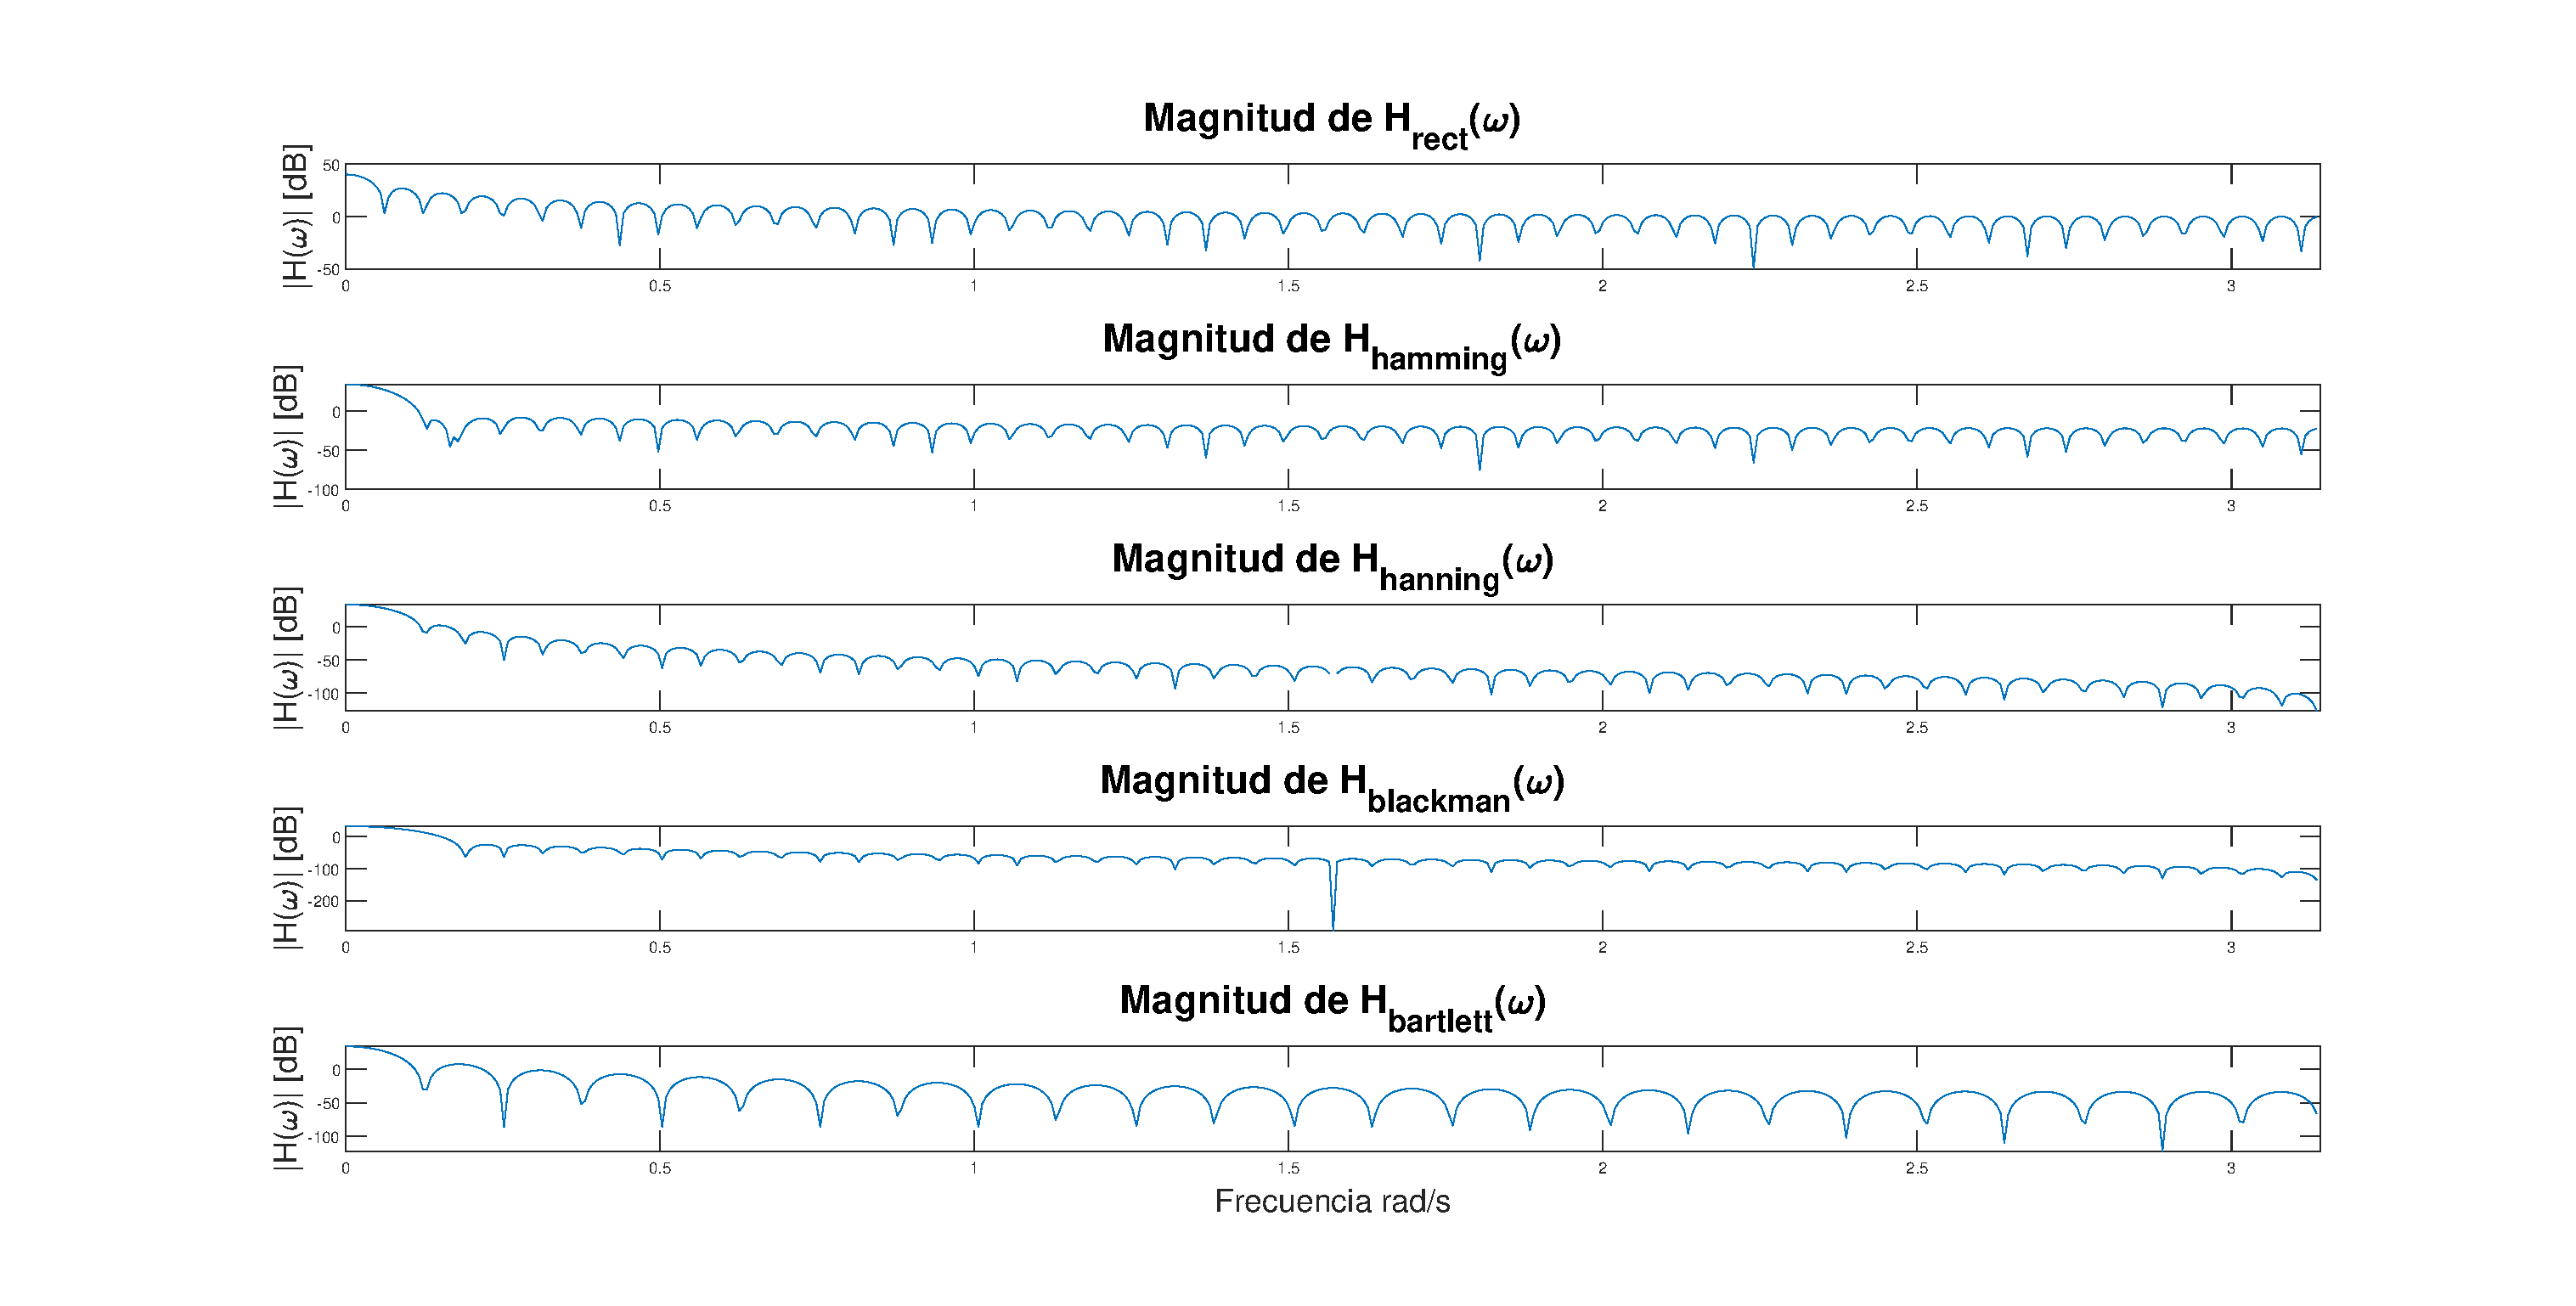
\includegraphics[scale = 0.3]{Figuras/p2_2-Ventanas-frecuencia.eps}
    \caption{Magnitud de ventanas rectangular, hamming, hanning, blackman, y bartlett en frecuencia.}
    \label{ventanas-magnitud}
\end{figure}


En la figura \ref{vent-mag-fase} se observa el comportamiento de las ventanas en frecuencia con énfasis en las frecuencias cercanas a cero, donde se pueden observar el ancho del \textit{mainlobe} de la ventana, además de la fase correspondiente a la ventana.

\begin{figure}[H]
    \centering
    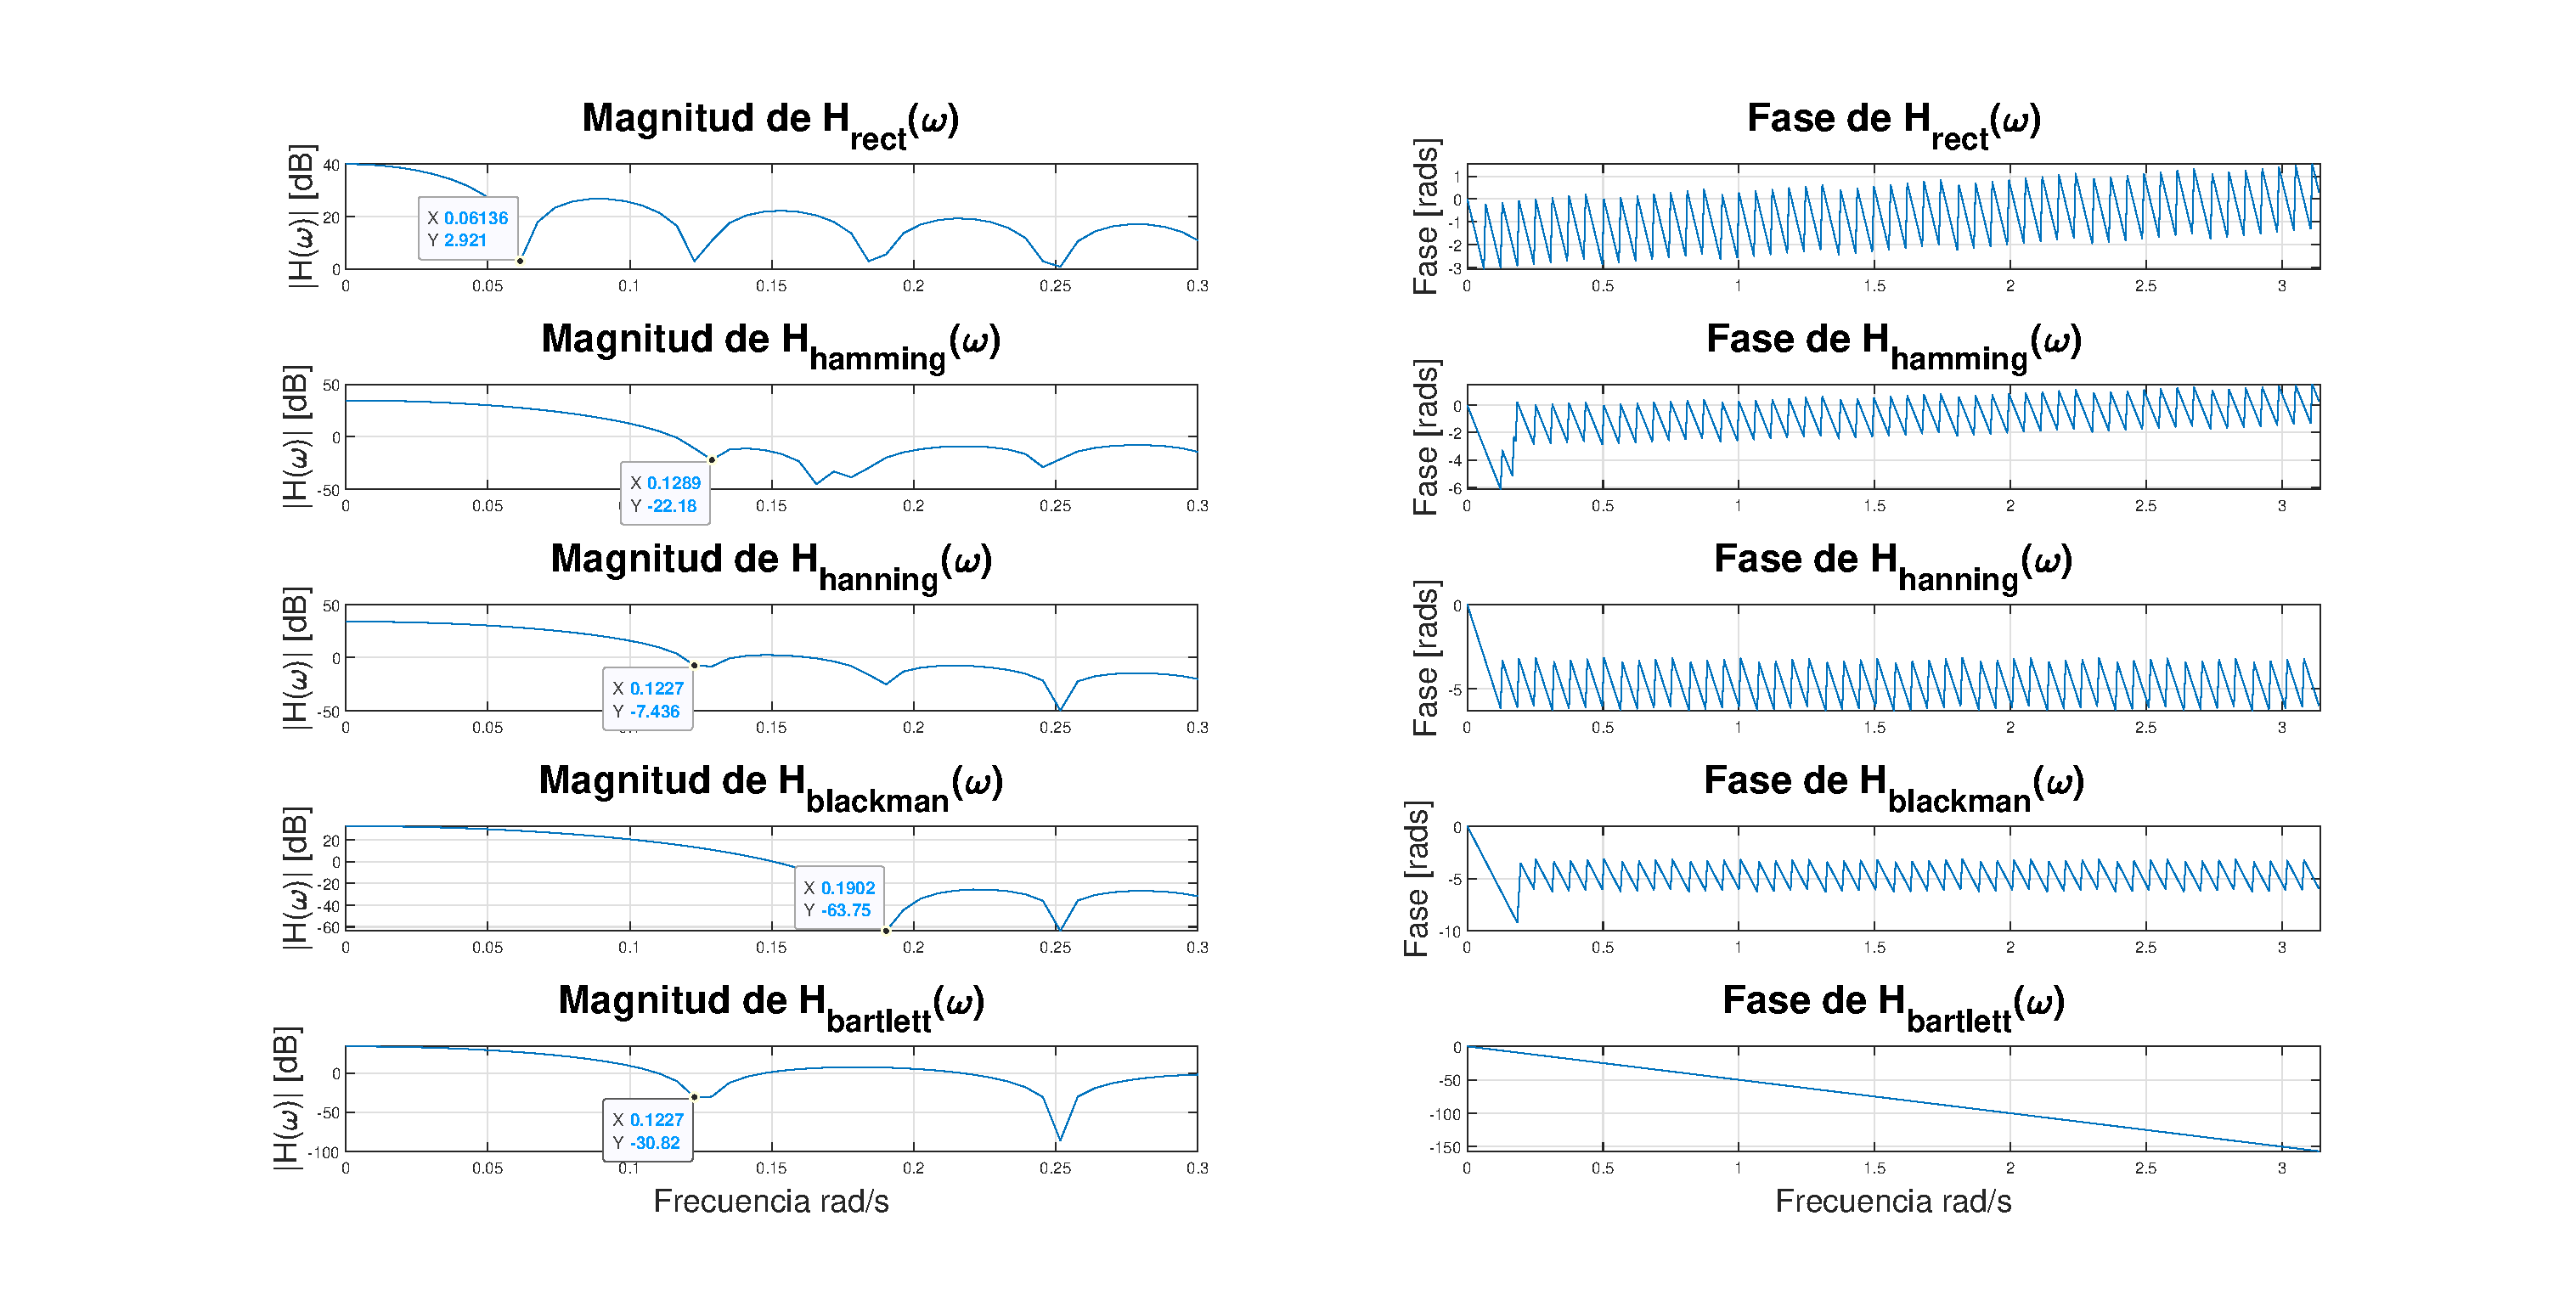
\includegraphics[scale = 0.3]{Figuras/p2_2-Magnitud-Fase.eps}
    \caption{Magnitud  y fase de ventanas rectangular, hamming, hanning, blackman, y bartlett en frecuencia. }
    \label{vent-mag-fase}
\end{figure}

En la figura \ref{lobulos}, se pueden ver los valores máximos que toman el \textit{mainlobe} y el \textit{sidelobe} para cada tipo de ventana, valores se resumen en el cuadro \ref{resumen_ventanas} junto al ancho del \textit{mainlobe}  de cada ventana obtenido anteriormente


\begin{figure}[H]
    \centering
    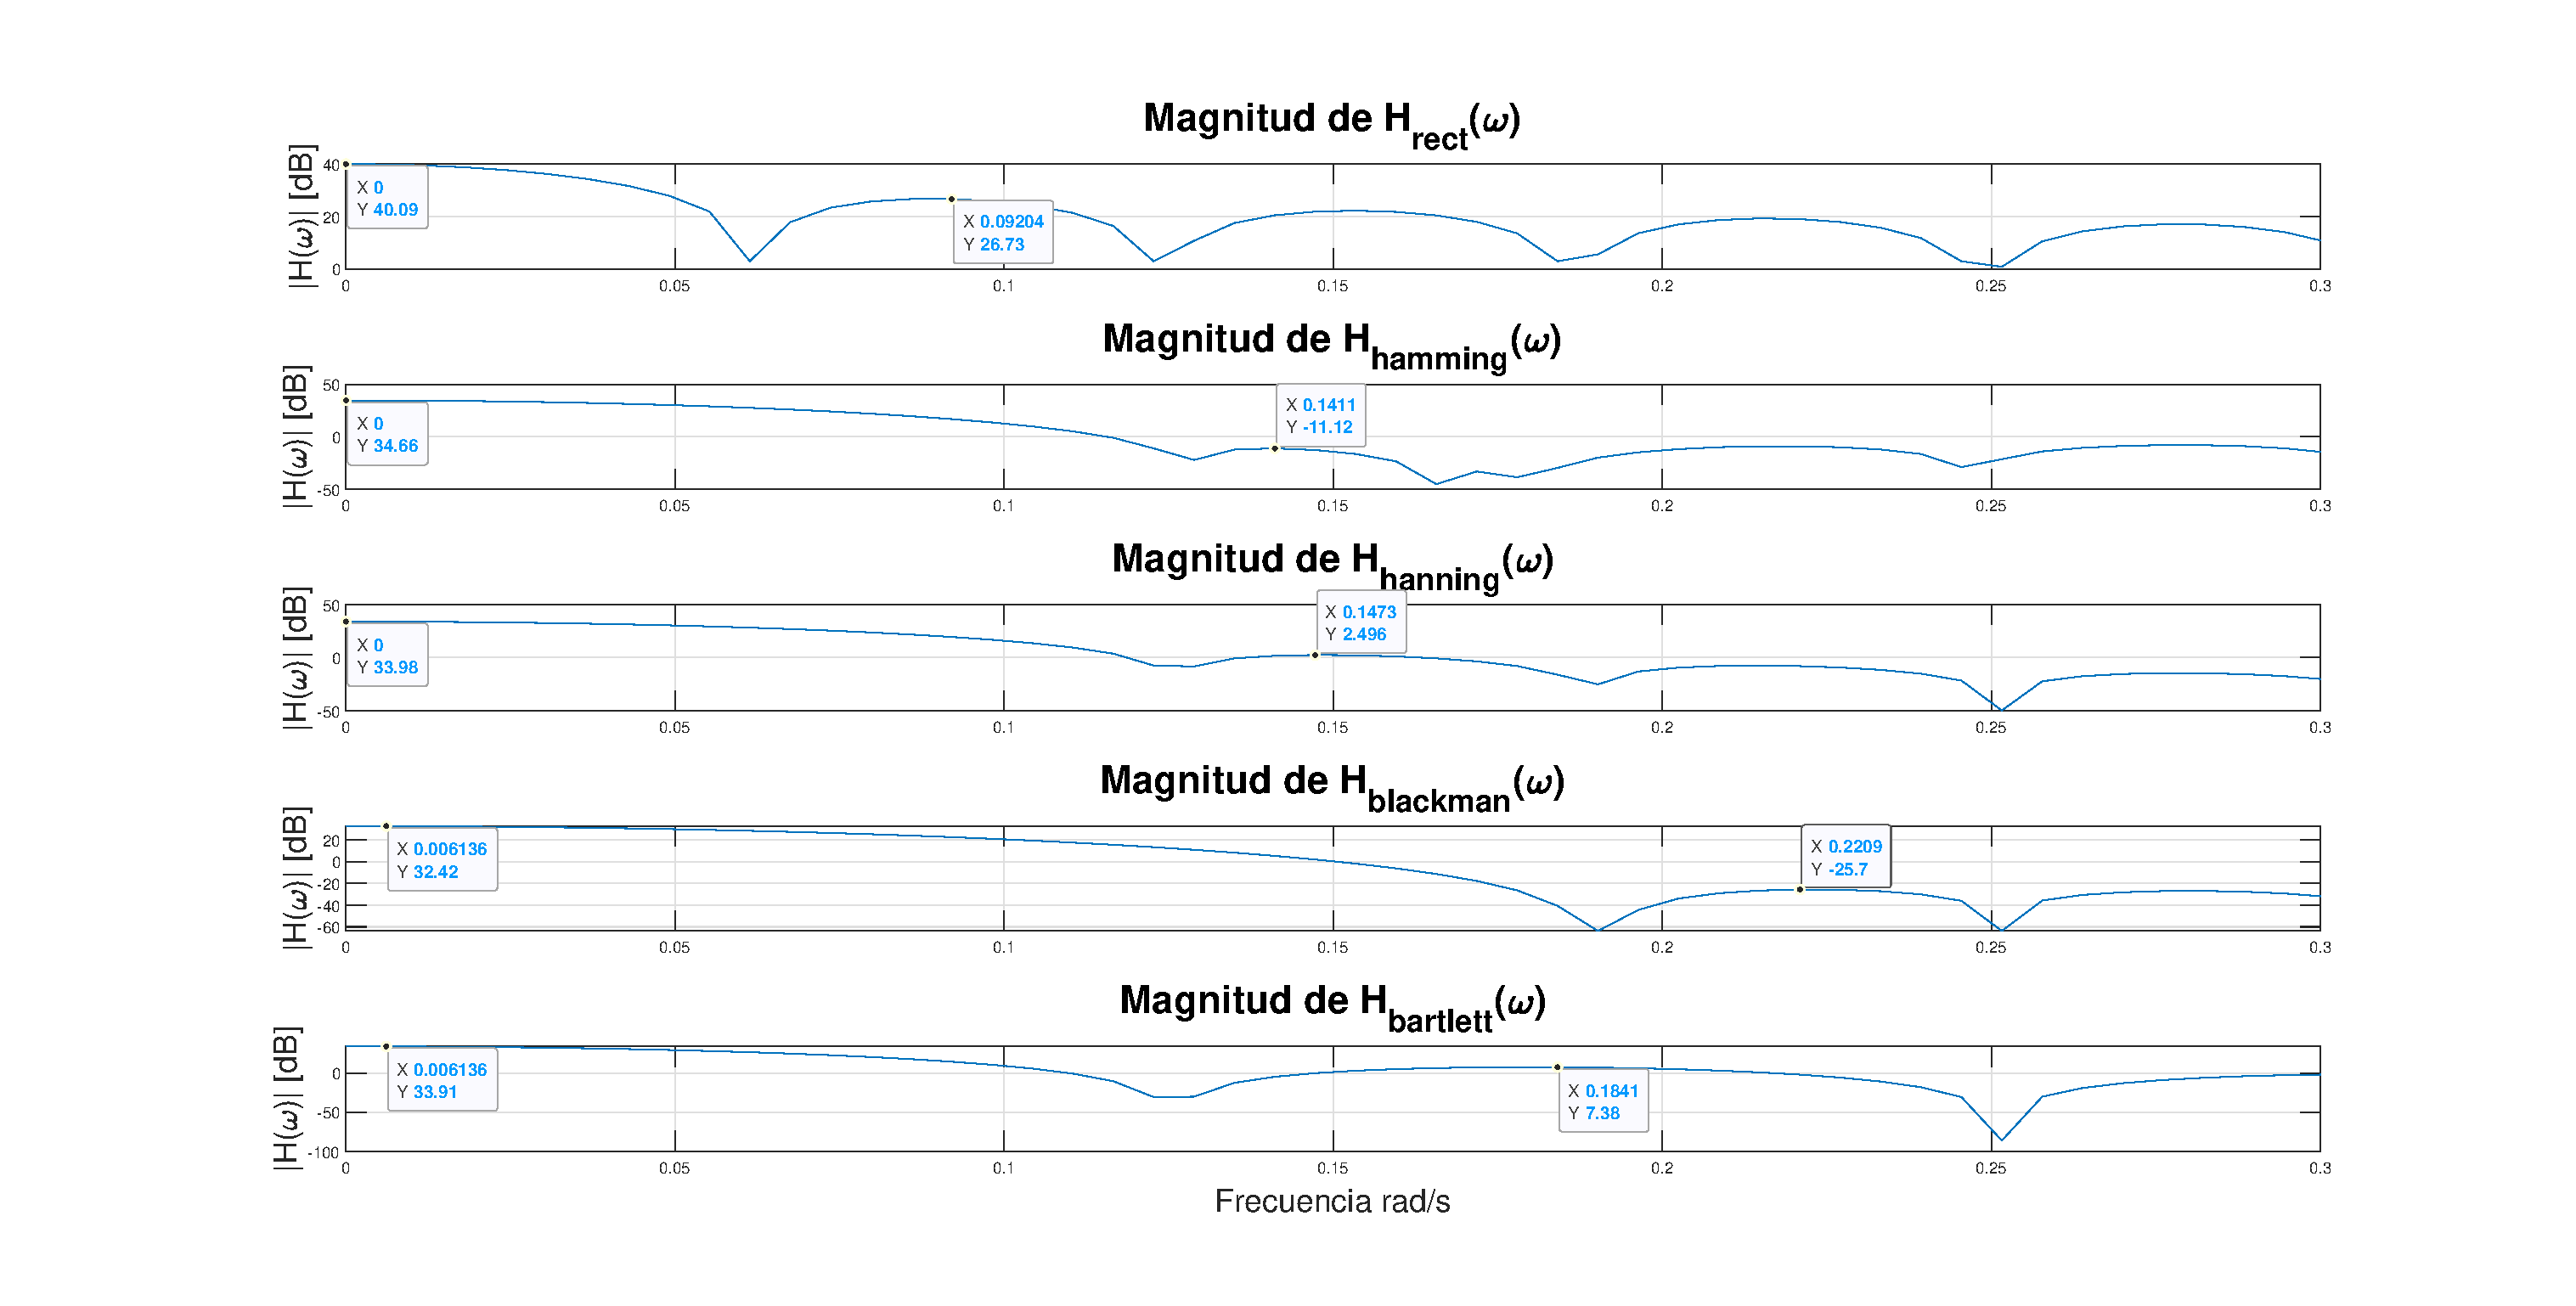
\includegraphics[scale = 0.3]{Figuras/p2_2-Lobulos.eps}
    \caption{Magnitud de ventanas rectangular, hamming, hanning, blackman, y bartlett en frecuencia identificando la amplitud del \textit{mainlobe} y el \textit{sidelobe}.}
    \label{lobulos}
\end{figure}


 Como todas las magnitudes se encuentran medidas en $db$ para encontrar la amplitud relativa de el \textit{sidelobe} basta con hacer la resta de la amplitud de este último con la amplitud del \textit{mainlobe}
 
 \begin{table}[H]
        \centering
        \begin{tabular}{|c|c|c|c|c|c|c|}
        \hline
         Ventana   & Ancho mainlobe & Max mainlobe & Max sidelobe & Amplitud relativa sidelobe\\
         \hline
         Rectangular  & 0.06136	 &  40.09 &	26.73	& -13.36 \\
         \hline
         Hamming  & 0.1289 &	34.66	& -11.12 &	-45.78	 \\
         \hline
         Hanning & 0.1227	& 33.98 &	2.496 &	 -31.484  \\
         \hline
        
         Blackman  & 0.1902 &	32.42	& -25.7 &	-58.12\\
         \hline
        
        Bartlett  & 0.1227 &	33.91	& 7.38 &	-26.53	\\
         \hline

        \end{tabular}
        \caption{Ancho \textit{mainlobe} y relación entre amplitud de \textit{mainlobe} y  \textit{sidelobe} en $db$}
        \label{resumen_ventanas}
    \end{table}

     De la tabla anterior se observa que la ventana rectangular es la ventana que tiene un sidelobe con mayor amplitud relativa, es decir, en cuanto a eficacia del filtro este es el menos óptimo.  Los filtros que poseen una mayor atenuación para las frecuencias fuera de su frecuencia de corte son los implementados con ventanas \textit{Hamming} y \textit{Blackman}, pero cabe mencionar que esta última compromete el ancho del lóbulo principal para lograr la atenuación que provee, esto podría generar conflictos dependiendo de lo que se busca en la implementación del filtro.  Los filtros con ventanas de tipo \textit{Hanning} y \textit{Bartlett} tienen un desempeño intermedio entre  el desempeño de ventana rectangular y el desempeño con ventanas \textit{Hamming} y/o \textit{Blackman}.

\end{enumerate}
\clearpage


\section{Diseño de Filtros FIR usando herramientas de MATLAB}

Inicialmente se lee sobre las herramientas de diseños FIR en MATLAB \texttt{fir1}, \texttt{fir2} y \texttt{firpm}. Sobre dichos comandos se puede comentar que:
\begin{itemize}
    \item \texttt{fir1}: Diseño de filtro FIR basado en ventanas. Retorna los coeficientes $b$ de un filtro FIR en base a un orden dado, una ventana y el tipo que se requiera. 
    %b = fir1(n,Wn,ftype) designs a lowpass, highpass, bandpass, bandstop, or multiband filter, depending on the value of ftype and the number of elements of Wn.
    \item \texttt{fir2}: Diseño de filtro FIR basado en muestreo de la respuesta en frecuencia. Retorna los coeficientes $b$ de un filtro FIR en base a un orden dado y a un set de puntos de la magnitud de la respuesta en frecuencia. 
    %b = fir2(n,f,m) returns an nth-order FIR filter with frequency-magnitude characteristics specified in the vectors f and m. The function linearly interpolates the desired frequency response onto a dense grid and then uses the inverse Fourier transform and a Hamming window to obtain the filter coefficients.
    \item \texttt{firpm}: Diseño de filtro FIR óptimo dado una respuesta en frecuencia deseada usando el algoritmo Parks-McClellan. En secciones posteriores se analizará más en detalle.
    %Parks-McClellan optimal FIR filter design
    %firpm designs a linear-phase FIR filter using the Parks-McClellan algorithm [2]. The Parks-McClellan algorithm uses the Remez exchange algorithm and Chebyshev approximation theory to design filters with an optimal fit between the desired and actual frequency responses. The filters are optimal in the sense that the maximum error between the desired frequency response and the actual frequency response is minimized.
\end{itemize}

\begin{enumerate}
\item En primer lugar se diseñan filtros FIR de orden 70, frecuencia de corte 3 kHz y frecuencia de muestreo 16 kHz, usando ventana rectangular y blackman, con el comando \texttt{fir1}.

La sección de código utilizada se muestra a continuación.
\begin{lstlisting}[frame=single]
%%% 1. Diseno de filtros FIR usando fir1

%orden
n1 = 70;
%frecuencia de corte normalizada
Fs = 16000; fc_Hz = 3000; fc = fc_Hz/(Fs/2);
%ventanas
win11 = ones(n1+1,1);win12 = blackman(n1+1);
%diseno
a1 =[1 zeros(1,n1-1)];
b11 = fir1(n1,fc,win11); b12 = fir1(n1,fc,win12);
\end{lstlisting}

Los gráficos de la respuesta en frecuencia de los filtros diseñados con ventana rectangular y blackman se muestran en las figuras \ref{fig:p3_1_rect} y \ref{fig:p3_1_blackman} respectivamente. Se aprecia que:
\begin{itemize}
    \item En el caso del filtro diseñado con ventana de rectangular se observa una región de transición más corta y menos atenuación en la banda de rechazo.
    \item El filtro diseñado con ventana blackman presenta una atenuación mayor en la banda de rechazo.
    %\item La región de fase lineal es mayor en el filtro diseñado con ventana blackman. Cabe destacar que en temas prácticos esta ventaja debiese ser poco notoria ya que la región de fase no lineal se encuentra en la banda de rechazo y por lo tanto es poco probable que se aprecie una distorsión significativa en la forma de onda.
\end{itemize}

\begin{figure}[H]
    \centering
    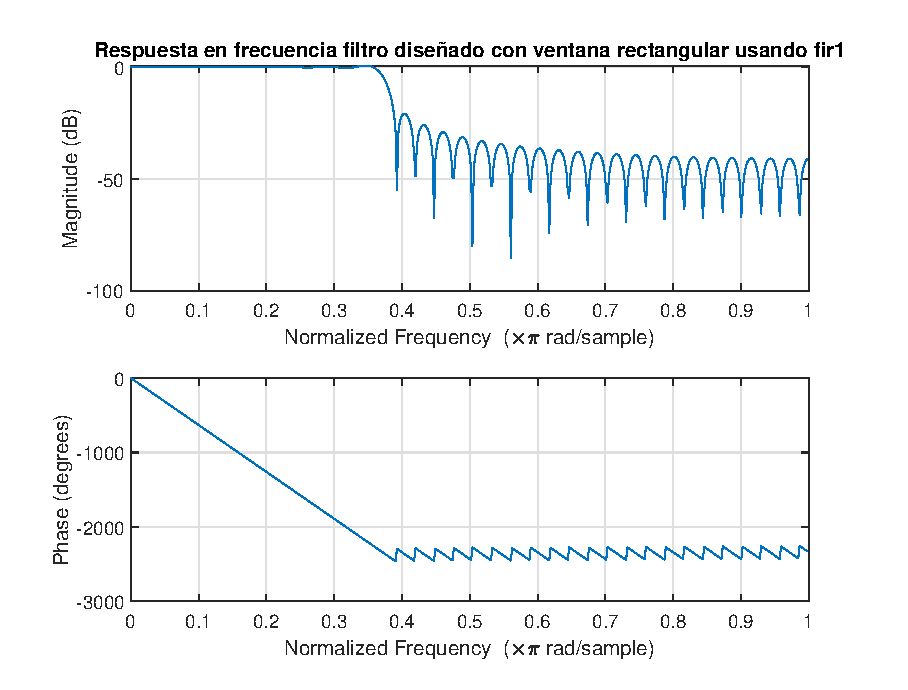
\includegraphics[width = .8 \linewidth]{Figuras/p1_31_rect.eps}
    \caption{Respuesta en frecuencia filtro diseñado con ventana rectangular usando \texttt{fir1}.}
    \label{fig:p3_1_rect}
\end{figure}
\begin{figure}[H]
    \centering
    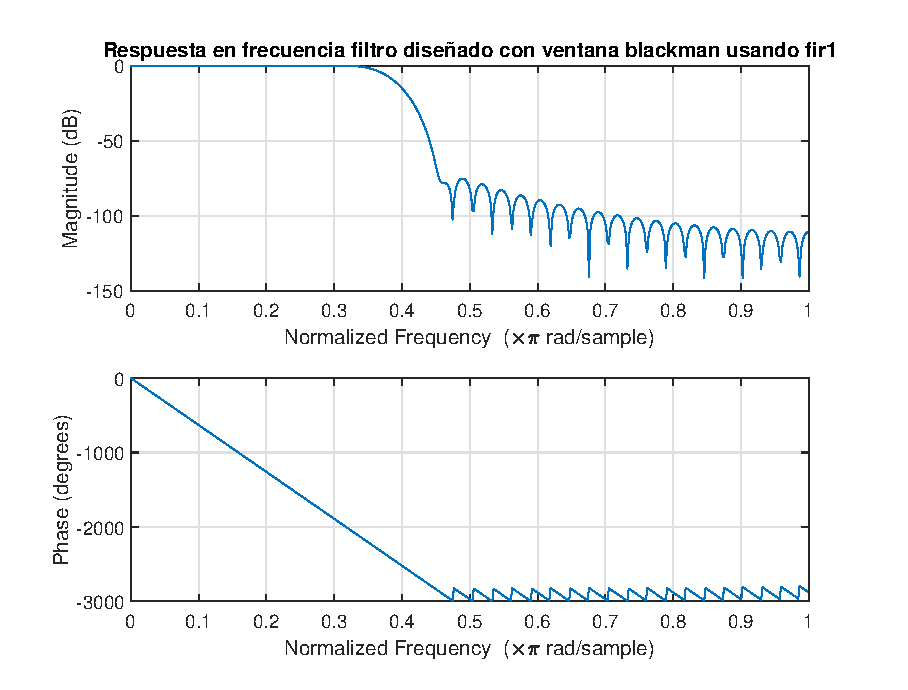
\includegraphics[width = .8 \linewidth]{Figuras/p1_31_blackman.eps}
    \caption{Respuesta en frecuencia filtro diseñado con ventana blackman usando \texttt{fir1}.}
    \label{fig:p3_1_blackman}
\end{figure}

\item Se pide encontrar el filtros de orden 70 y 150 usando el comando \texttt{fir2} de MATLAB, el cual recibe el orden del filtro y un set de puntos de respuesta en frecuencia los cuales son interpolados linealmente. La respuesta en frecuencia ideal a emular se muestra en la figura \ref{fig:p3_2_obj}
\begin{figure}[H]
    \centering
    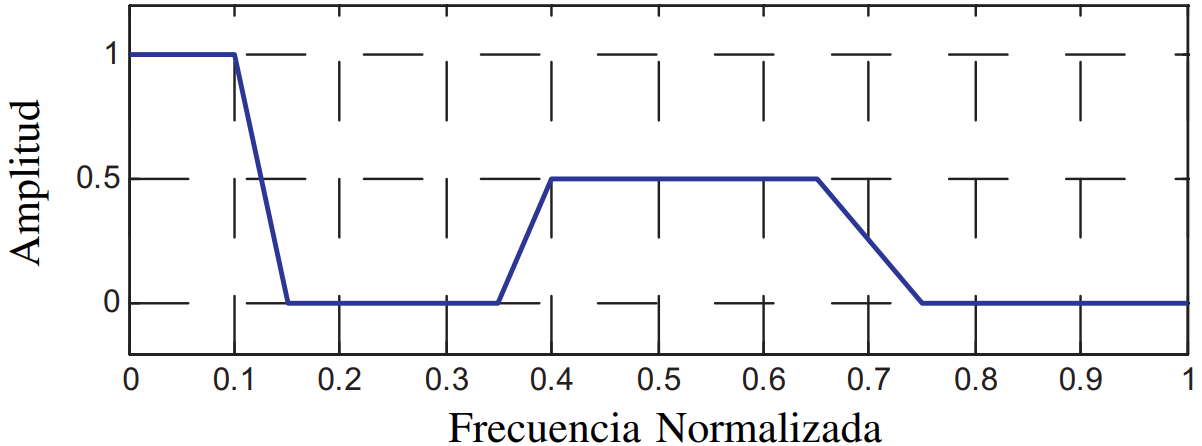
\includegraphics[width = .8 \linewidth]{Figuras/p3_2_obj.png}
    \caption{Respuesta en frecuencia ideal a emular.}
    \label{fig:p3_2_obj}
\end{figure}

La sección de código con la cual se diseñan los filtros se muestra a cotinuación:
\begin{lstlisting}[frame = single]
%%% 2. Diseno de filtros FIR usando fir2

%orden 
n21 = 70; n22 = 150;
%Objetivo en frecuencia
f_obj = [0 .1 .15 .35 .4 .65 .75 1];
h_obj = [1  1   0   0 .5  .5   0 0];
%diseno
b21 = fir2(n21,f_obj, h_obj); b22 = fir2(n22,f_obj, h_obj);
\end{lstlisting}
donde simplemente se reconocieron los puntos en la respuesta en frecuencia tal que al interpolar linealmente se llegara a la respuesta en frecuencia ideal.

En primer lugar se grafica la magnitud de la respuesta en frecuencia del filtro ideal y los 2 diseñados, lo cual se muestra en la figura \ref{fig:p3_2_fr1}. Se aprecia un diseño correcto según las especificaciones en frecuencia.
\begin{figure}[H]
    \centering
    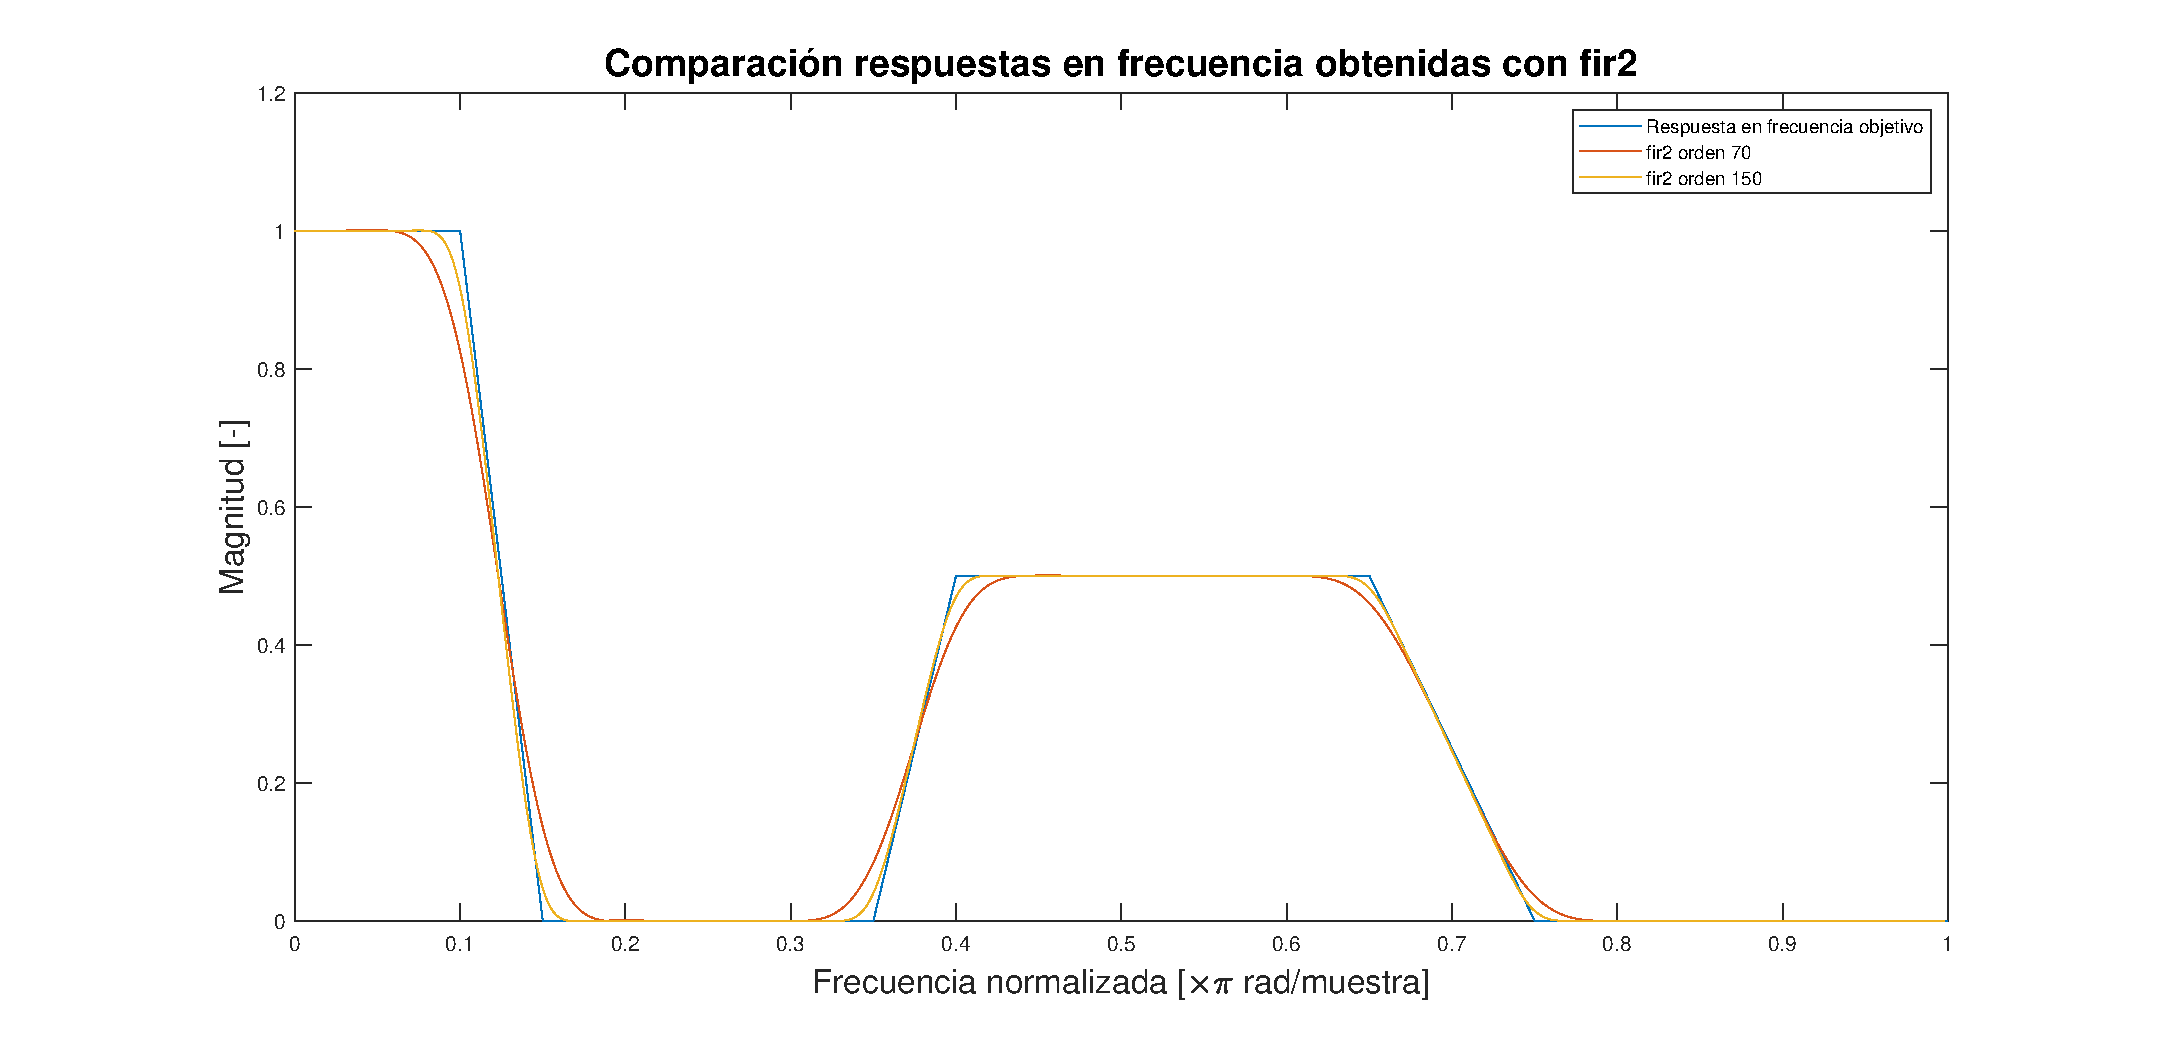
\includegraphics[width = .8 \linewidth]{Figuras/p1_32_FR1.eps}
    \caption{Magnitud de la respuesta en frecuencia de filtro ideal y de diseñados con \texttt{fir2}.}
    \label{fig:p3_2_fr1}
\end{figure}
Posteriormente, para una mejor comparación entre la respuesta en frecuencia de ambos filtros diseñados, se grafica la magnitud de la respuesta en frecuencia en dB, lo cual se muestra en la figura \ref{fig:p3_2_fr2}. 

Se aprecia que no hay gran diferencia en atenuación entre ambos filtros, siendo obviamente el filtro de mayor orden de atenuación más fuerte. La mayor diferencia se aprecia en la banda de transición, la cual es claramente mas abrupta en el filtro de mayor orden. Dependiendo la aplicación esa podría ser una ventaja a considerar.
\begin{figure}[H]
    \centering
    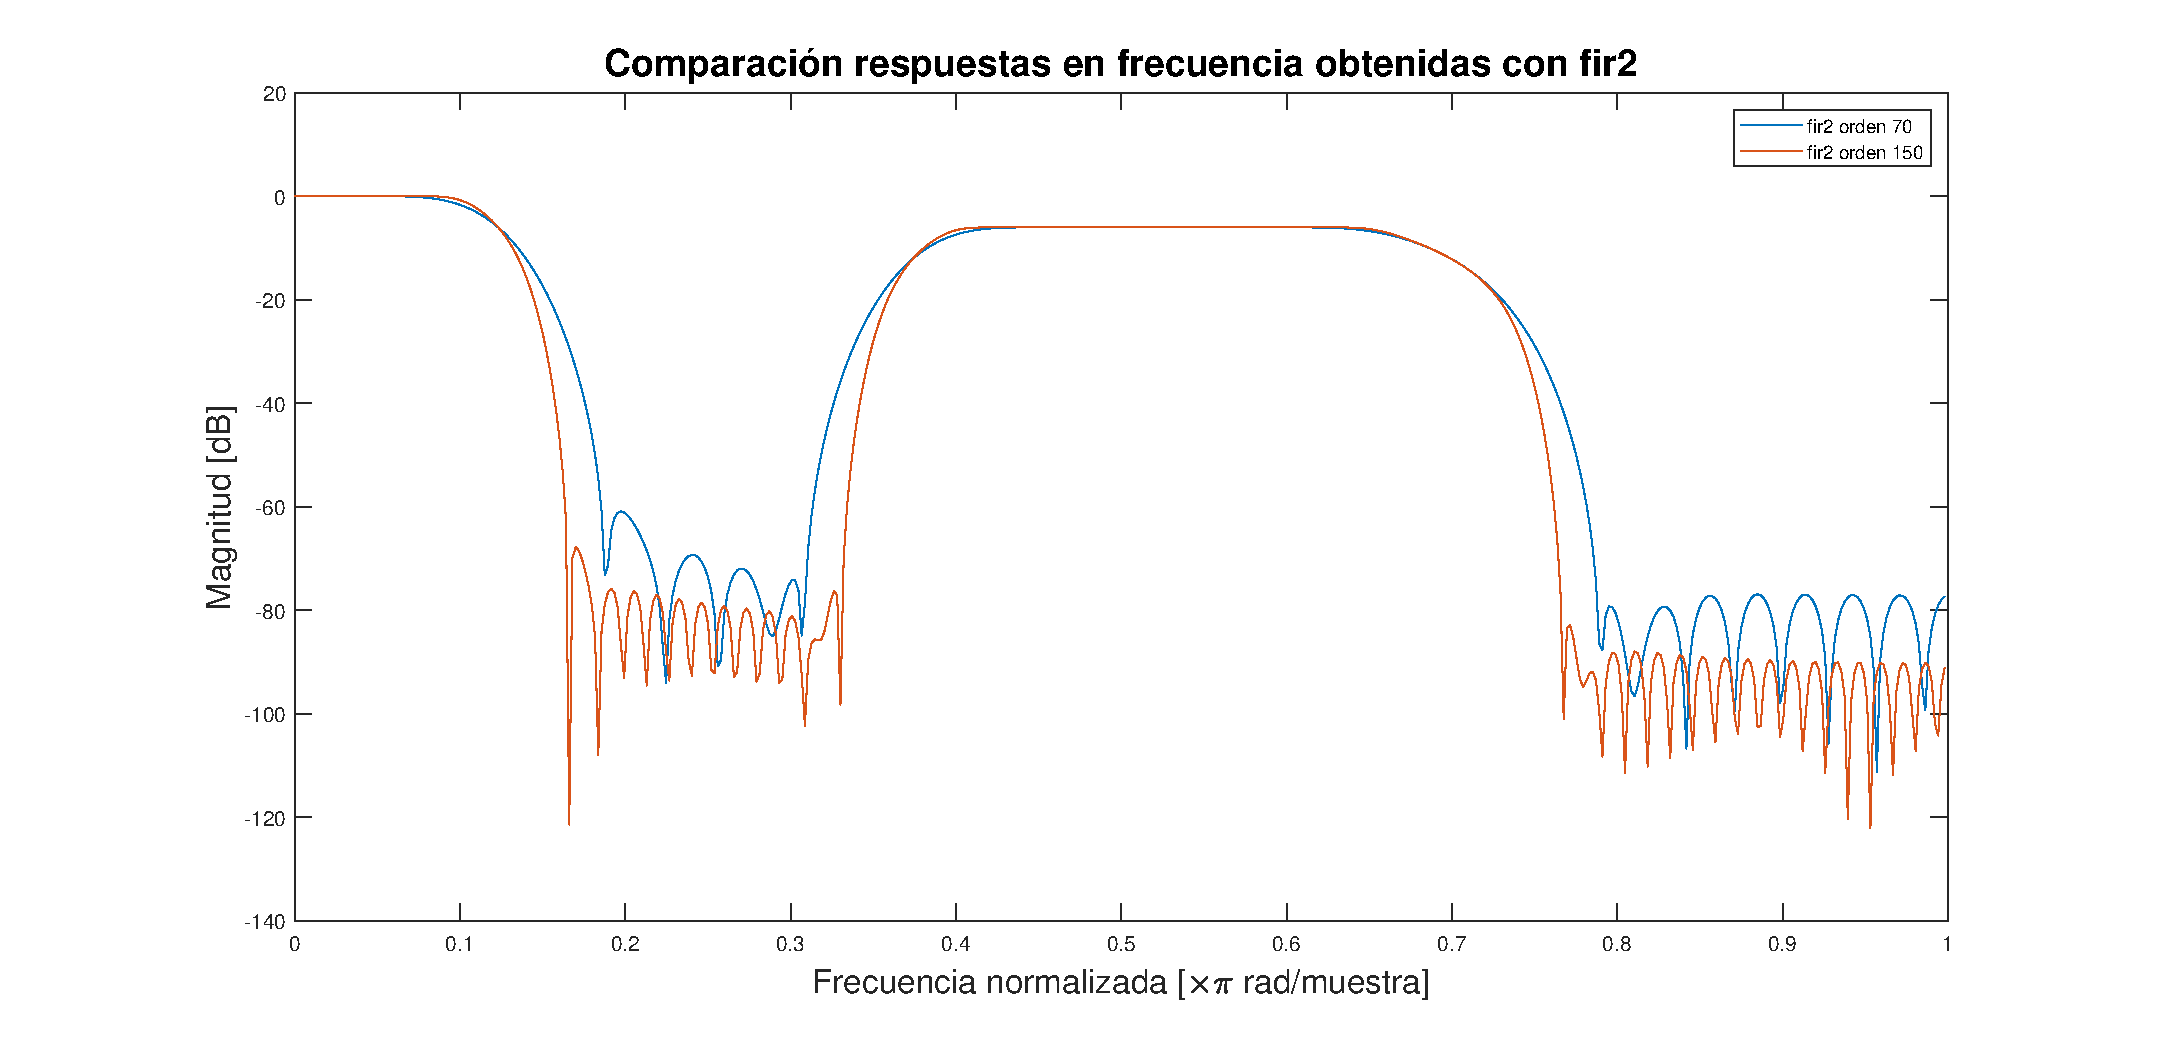
\includegraphics[width = .8 \linewidth]{Figuras/p1_32_FR2.eps}
    \caption{Magnitud de la respuesta en frecuencia de filtro ideal y de diseñados con \texttt{fir2} en dB.}
    \label{fig:p3_2_fr2}
\end{figure}
\item El comando \texttt{firpm} hace referencia al diseño de filtro FIR ocupando el algoritmo Parks-McClellan.

Dicho algoritmo corresponde a un método iterativo para el diseño óptimo de filtros FIR dada una respuesta en frecuencia deseada y sujeto a un orden. Cabe destacar que el criterio de  optimalidad es en el sentido de la norma $\infty$ del error en frecuencia o, en otras palabras, del máximo error absoluto entre la respuesta en frecuencia deseada y la respuesta frecuencia obtenida situando los ceros del filtro.

La sintaxis típica del comando es \texttt{b = firpm(n,f,a)} donde:
\begin{itemize}
    \item \texttt{b}: Vector de coeficientes MA del filtro FIR.
    \item \texttt{n}: Orden del filtro a diseñar.
    \item \texttt{f}: Vector de frecuencias.
    \item \texttt{a}: Vector de amplitudes de la respuesta en frecuencia correspondientes al vector de frecuencias.
\end{itemize}

Una forma de utilizar este comando es en el diseño de filtros chebyshev cuando existe una restricción de ripple para obtener un filtro de bajo orden.

Para lo anterior en primer lugar se ocuparía el comando \texttt{firmord} para estimar el orden del filtro óptimo dada una respuesta en frecuencia deseada junto a sus restricciones de ripple y luego ocupar esa misma respuesta en frecuencia deseada junto con el orden obtenido para la obtención de los coeficientes de \texttt{b} usando \texttt{firpm}.


%\texttt{firpm}: Diseño de filtro FIR óptimo dado una respuesta en frecuencia deseada usando el algoritmo Parks-McClellan. En secciones posteriores se analizará más en detalle.
%Parks-McClellan optimal FIR filter design
%firpm designs a linear-phase FIR filter using the Parks-McClellan algorithm [2]. The Parks-McClellan algorithm uses the Remez exchange algorithm and Chebyshev approximation theory to design filters with an optimal fit between the desired and actual frequency responses. The filters are optimal in the sense that the maximum error between the desired frequency response and the actual frequency response is minimized.
\end{enumerate}
\clearpage

\section{Diseño de Filtros  IIR usando herramientas de MATLAB}
\begin{enumerate}
\item En primer lugar se diseñan 4 filtros elípticos usando el comando \texttt{ellip} de MATLAB. Las especificacones de dichos filtros son:
\begin{itemize}
    \item Filtro a: Pasa bajos orden 2 ($f_c = 2 kHz$).
    \item Filtro b: Pasa altos orden 2 ($f_c = 4 kHz$)
    \item Filtro c: Pasa banda orden 4 ($f_1 = 2 kHz, f_2 = 4 kHz$)
    \item Filtro d: Elimina banda orden 4 ($f_1 = 2 kHz, f_2 = 4 kHz$)
\end{itemize}
como suposición se escogió:
\begin{itemize}
    \item Ripple en banda de paso: 5 dB.
    \item Atenuación en banda de rechazo: 20 dB.
\end{itemize}

La sintaxis típica del comando \texttt{ellip} es: \texttt{[b,a] = ellip(n,Rp, Rs, Wn, Ftype)} donde:
\begin{itemize}
    \item \texttt{b}: Coeficientes de la parte MA del filtro.
    \item \texttt{a}: Coeficientes de la parte AR del filtro.
    \item \texttt{n}: Orden del filtro
    \item \texttt{Rp}: Ripple máximo tolerado en banda de paso.
    \item \texttt{Rs}: Atenuación en banda de rechazo
    \item \texttt{Wn}: Frecuencia o frecuencias de corte en $\pi\cdot$rad/muestra
    \item \texttt{Ftype}: Tipo de filtro (pasa bajos, pasa altos, pasabanda o elimina banda).
\end{itemize}

Con las suposiciones tomadas y las condiciones del diseño del filtro se diseñan los filtros usando el siguiente segmento de código:
\begin{lstlisting}[frame=single]
%%% 1. Diseno de filtros IIR usando ellip

%ordenes
n1a = 2; n1b = 2; n1c = 4; n1d = 4;
%frecuencias de corte normalizadas (pasa bajos y pasa altos)
Fs = 16000; fc1_a1_Hz = 2000; fc1_a1 = fc1_a1_Hz/Fs;%filtro a
fc1_b1_Hz = 4000; fc1_b1 = fc1_b1_Hz/Fs;            %filtro b
%frecuencias normalizadas (pasa banda y elimina banda)
f1_c1_Hz = 2000; f1_c1 = f1_c1_Hz/Fs;               %filtro c
f1_c2_Hz = 4000; f1_c2 = f1_c2_Hz/Fs;
f1_d1_Hz = 2000; f1_d1 = f1_d1_Hz/Fs;               %filtro d
f1_d2_Hz = 4000; f1_d2 = f1_d2_Hz/Fs;
%Suposiciones de ripple y banda de rechazo
Rp = 5; Rs = 20; %Ripple banda de paso y atenuacion (rechazo)  
%Diseno de Filtros 
[b1_a, a1_a]=ellip(n1a, Rp, Rs, 2*fc1_a1, "low");
[b1_b, a1_b]=ellip(n1b, Rp, Rs, 2*fc1_b1, "high");
[b1_c, a1_c]=ellip(n1c, Rp, Rs, 2*[f1_c1 f1_c2], "bandpass");
[b1_d, a1_d]=ellip(n1d, Rp, Rs, 2*[f1_d1 f1_d2], "stop");
\end{lstlisting}

Las respuestas en frecuencia de los filtros diseñados se muestran en las figuras \ref{fig:p4_1a}, \ref{fig:p4_1b}, \ref{fig:p4_1c} y \ref{fig:p4_1d}. Se aprecia que se cumplen los requisitos de diseño.
\begin{figure}[H]
    \centering
    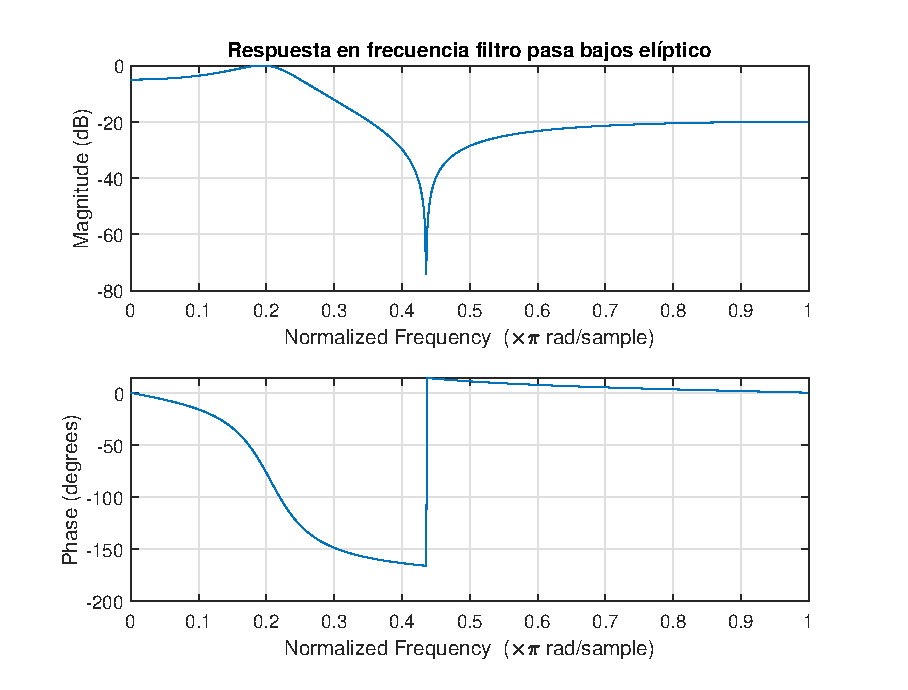
\includegraphics[width = .8\linewidth]{Figuras/p4_1a.eps}
    \caption{Respuesta en frecuencia de filtro pasa bajos diseñado usando \texttt{ellip}, de orden 2, $f_c = 2 kHz$, ripple en banda de paso 5 dB y atenuación de 20 dB en banda de rechazo.}
    \label{fig:p4_1a}
\end{figure}

\begin{figure}[H]
    \centering
    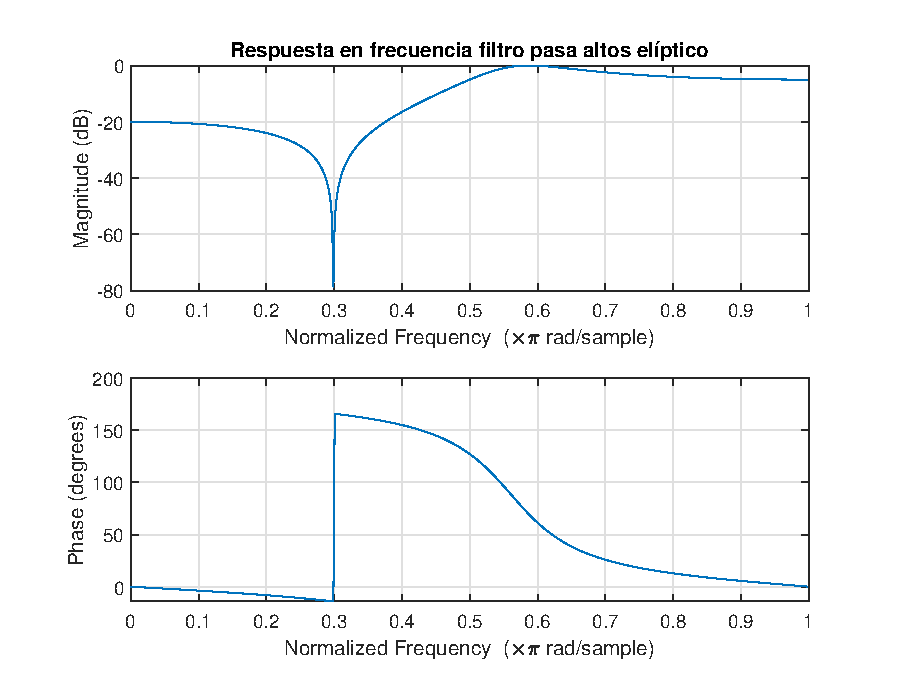
\includegraphics[width = .8\linewidth]{Figuras/p4_1b.eps}
    \caption{Respuesta en frecuencia de filtro pasa altos diseñado usando \texttt{ellip}, de orden 2, $f_c = 4 kHz$, ripple en banda de paso de 5 dB y atenuación de 20 dB en banda de rechazo.}
    \label{fig:p4_1b}
\end{figure}

\begin{figure}[H]
    \centering
    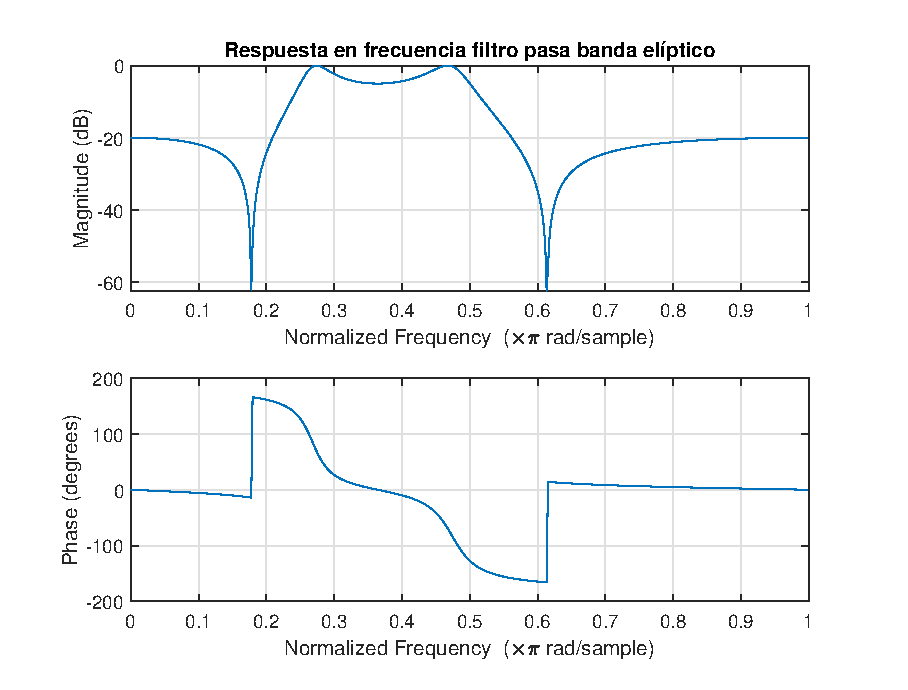
\includegraphics[width = .8\linewidth]{Figuras/p4_1c.eps}
    \caption{Respuesta en frecuencia de filtro pasa banda diseñado usando \texttt{ellip}, de orden 4, $f_1 = 2 kHz, f_2= 4 kHz$, ripple en banda de paso de 5 dB y atenuación de 20 dB en banda de rechazo.}
    \label{fig:p4_1c}
\end{figure}

\begin{figure}[H]
    \centering
    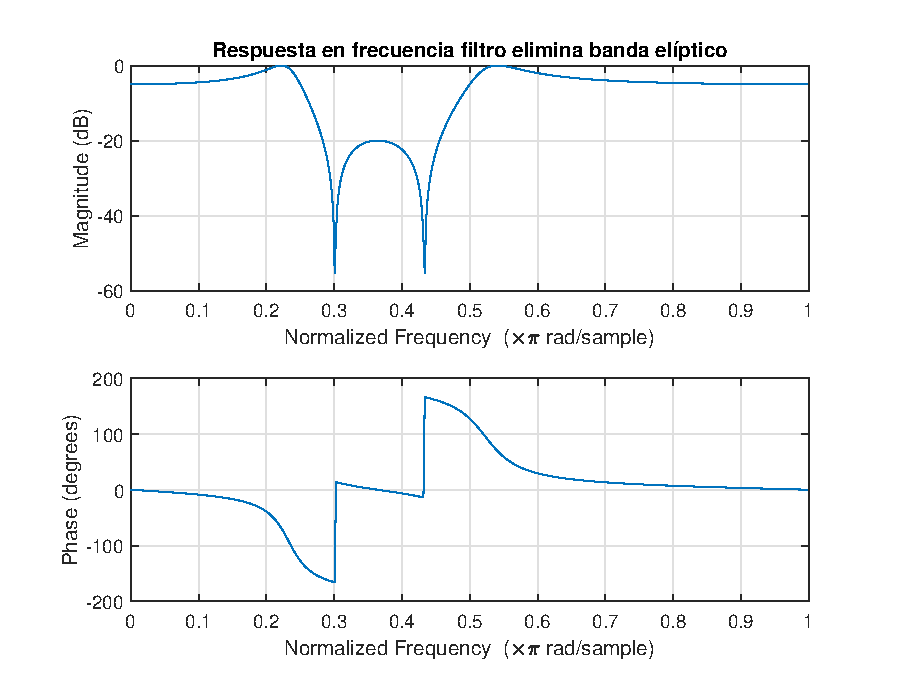
\includegraphics[width = .8\linewidth]{Figuras/p4_1d.eps}
    \caption{Respuesta en frecuencia de filtro elimina banda diseñado usando \texttt{ellip}, de orden 4, $f_1 = 2 kHz, f_2= 4 kHz$, ripple en banda de paso de 5 dB y atenuación de 20 dB en banda de rechazo.}
    \label{fig:p4_1d}
\end{figure}

\item Se pide diseñar 2 filtros pasabanda usando los comandos de MATLAB \texttt{cheby1} y \texttt{cheby2}, considerando frecuencias de corte $f_1 = 2$ kHz y $f_2 = 4$  kHz, una frecuencia de muestreo de 16 kHz y orden 4.

Para un filtro se pide 2 dB máximo de ripple en la banda de paso y para el otro 20 dB de atenuación en la banda de rechazo. Debido a que el filtro de chebishev tipo I es un filtro que permite una región de transición corta dado un máximo de ripple en la banda de paso se uso \texttt{cheby1} para el primer filtro. Para el segundo se usó \texttt{cheby2} pues el filtro de chebishev tipo II  permite asegurar un mínimo de atenuación.

La sección de código para el diseño de los filtros se muestra a continuación

\begin{lstlisting}[frame=single]
%% 2. Diseno de filtros chebyshev tipo I y II

%orden
n2 = 4;
%frecuencias de corte
f2_1_Hz = 2000; f2_1 = f2_1_Hz/Fs;
f2_2_Hz = 4000; f2_2 = f2_2_Hz/Fs;
%Restricciones de Ripple
Rp = 2; Rs = 20;
%Diseno de Filtros [b,a] = cheby1(n,Rp,Wp,ftype)
[b2_a, a2_a] = cheby1(n2, Rp, 2*[f2_1 f2_2], "bandpass");
[b2_b, a2_b] = cheby2(n2, Rs, 2*[f2_1 f2_2], "bandpass");
\end{lstlisting}

Las imágenes de respuesta en frecuencia para el filtro a y b diseñados se muestran en las figuras \ref{} y \ref{} respectivamente. Se aprecia que se cumplen los requisitos de diseño.

\begin{figure}[H]
    \centering
    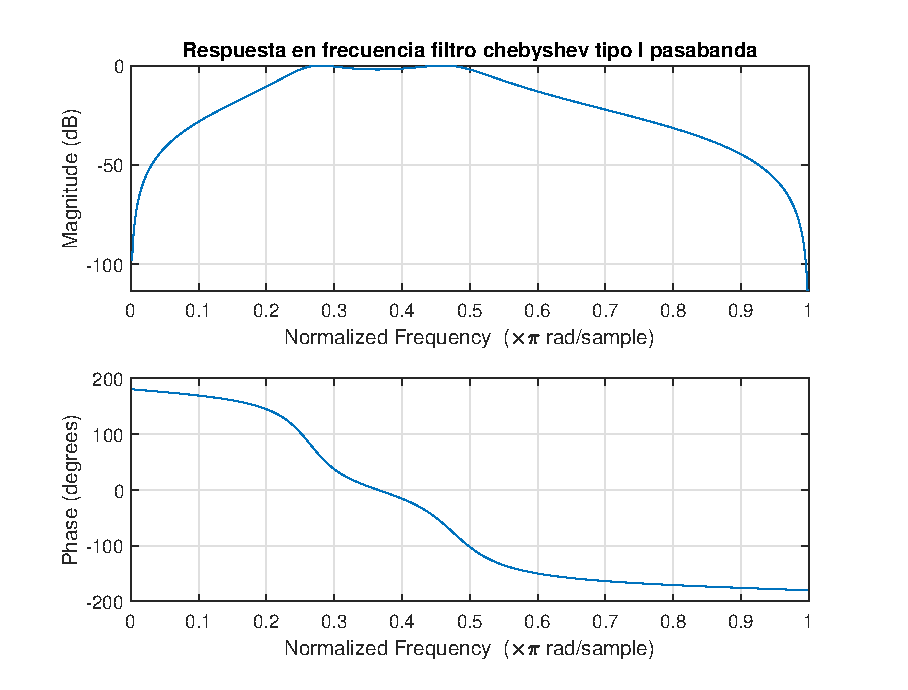
\includegraphics[width = .8\linewidth]{Figuras/p4_2a.eps}
    \caption{Respuesta en frecuencia de filtro pasa banda con ripple máximo de 2 dB en banda de paso, diseñado usando estructura de filtro chebyshev tipo I.}
    \label{fig:p4_2a}
\end{figure}

\begin{figure}[H]
    \centering
    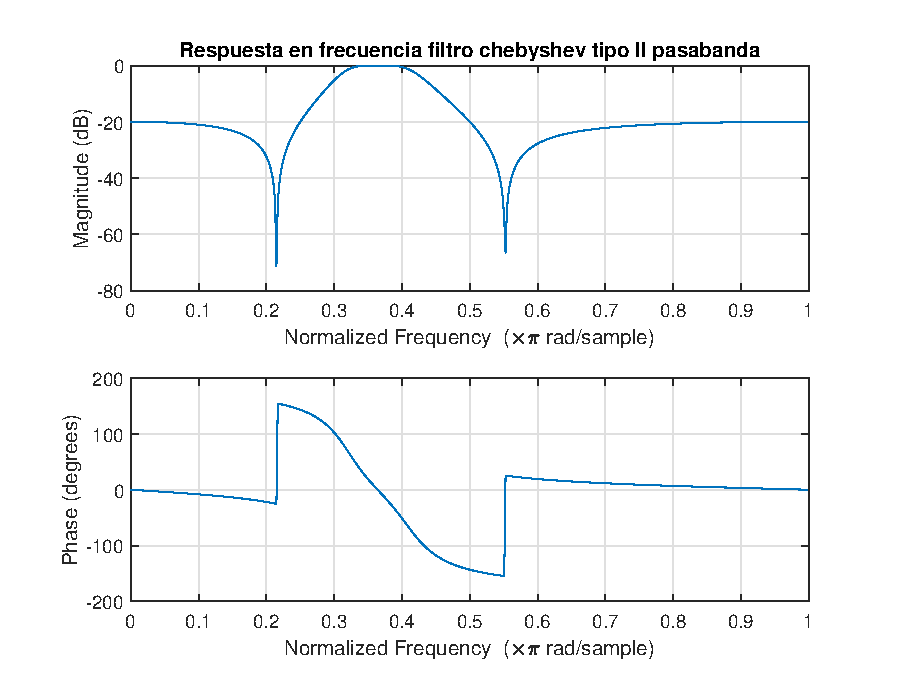
\includegraphics[width = .8\linewidth]{Figuras/p4_2b.eps}
    \caption{Respuesta en frecuencia de filtro pasa banda con atenuación mínima de 20 dB en banda de rechazo, diseñado usando estructura de filtro chebyshev tipo II.}
    \label{fig:p4_2b}
\end{figure}

De evaluar la respuesta en frecuencia del filtro chebyshev tipo I diseñado se obtiene que:
\begin{align*}
    h_{I}(f_1 = 2000 \text{ Hz}) &= h_{I}\left(0.25  \dfrac{\pi\text{rad}}{\text{sample}}\right) \approx -32.76 \text{ dB} \\
    h_{I}(f_1 = 4000 \text{ Hz}) &= h_{I}\left(0.5  \dfrac{\pi\text{rad}}{\text{sample}}\right) \approx -17.81 \text{ dB} \\
\end{align*}

De evaluar la respuesta en frecuencia del filtro chebyshev tipo II diseñado se obtiene que:
\begin{align*}
    h_{II}(f_1 = 2000 \text{ Hz}) &= h_{II}\left(0.25  \dfrac{\pi\text{rad}}{\text{sample}}\right) \approx -20.61 \text{ dB} \\
    h_{II}(f_1 = 4000 \text{ Hz}) &= h_{II}\left(0.5  \dfrac{\pi\text{rad}}{\text{sample}}\right) \approx -23.87 \text{ dB} \\
\end{align*}

\item Se pide diseñar un filtro butterworth pasa banda de orden 4, con frecuencias de corte $f_1 = 800$ Hz y $f_2 = 1600$ Hz usando el comando \texttt{butter}, considerando una frecuencia de muestreo de 16 kHz. La sección de código se muestra a continuación:
\newpage
\begin{lstlisting}[frame=single]
%%% 3. Diseno de filtros butterworth

%orden
n3 = 4/2;
%frecuencias de corte
f3_1_Hz = 800 ; f3_1 = f3_1_Hz/Fs;
f3_2_Hz = 1600; f3_2 = f3_2_Hz/Fs;
%Diseño de Filtros
[b3, a3] = butter(n3, 2*[f3_1 f3_2], "bandpass");
\end{lstlisting}

La respuesta en frecuencia del filtro diseñado se muestra en la figura \ref{fig:p4_3}.

\begin{figure}[H]
    \centering
    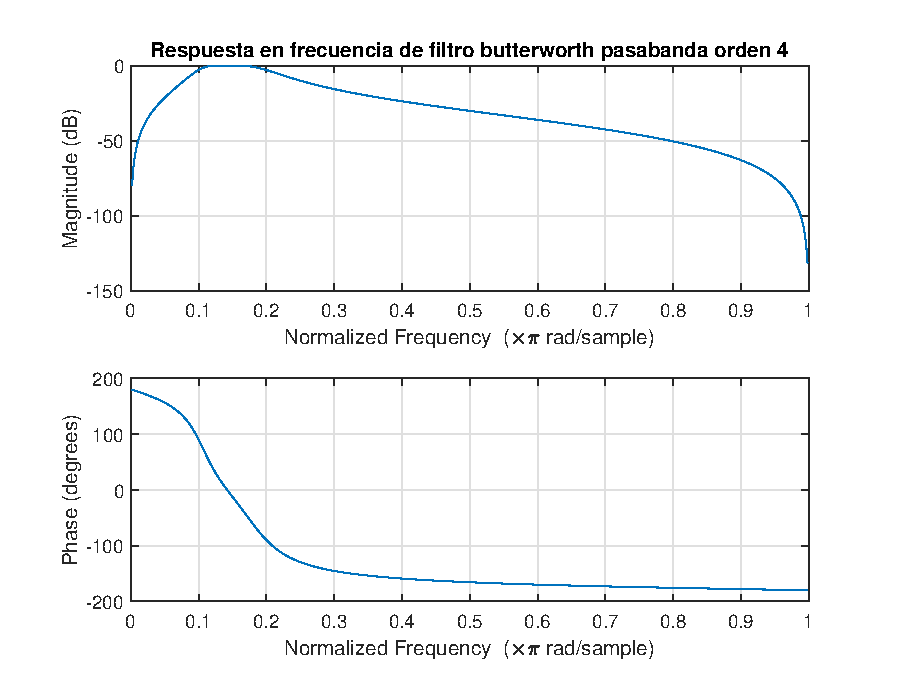
\includegraphics[width = .8\linewidth]{Figuras/p4_3.eps}
    \caption{Respuesta en frecuencia de filtro butterworth pasa banda de orden 4 diseñado.}
    \label{fig:p4_3}
\end{figure}

Posteriormente se hace un análisis de que ocurre con la ubicación de polos y ceros al diseñar filtros butterworth a medida que se aumenta el orden. La sección de código para aquello se muestra a continuación:
\begin{lstlisting}
%Analisis de polos y ceros butterworth 
n = [4 6 8 10 12 14];
figure
for i = 1:6
    [z,p,~] = butter(n(i)/2, 2*[f3_1 f3_2], "bandpass");
    subplot(3,2,i); zplane(z,p);
    title({"Diagrama de polos y ceros para filtro ", strcat(
        "butterworth pasabandas de orden ", int2str(n(i)))})
end
\end{lstlisting}

Los diagramas de polos y ceros se muestran en la figura \ref{fig:p4_3zp}. Notar que a medida que aumenta el orden del filtro los polos dominantes se acercan más al círculo unitario. Lo anterior podría volver el sistema inestable por temas numéricos.

\begin{figure}[H]
    \centering
    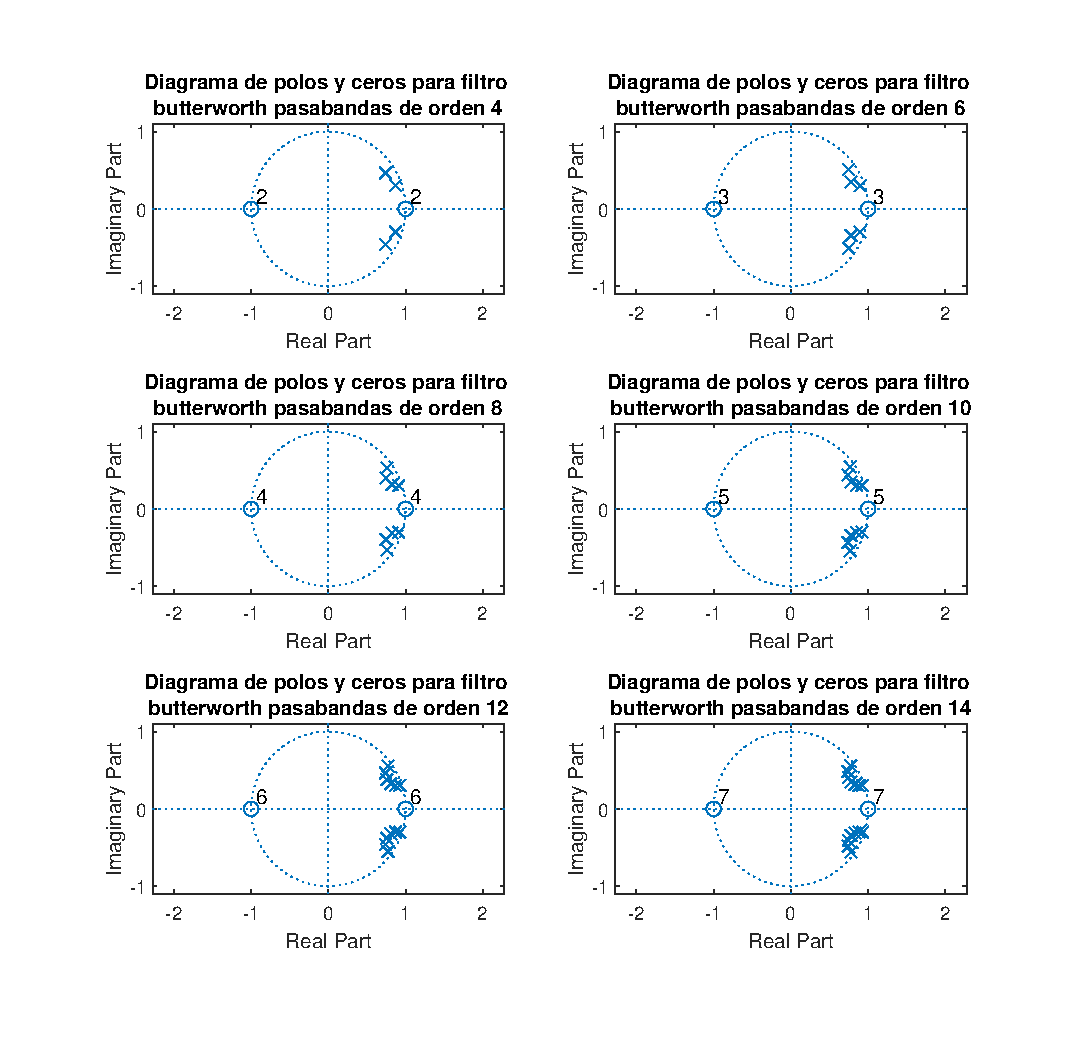
\includegraphics[width = .95\linewidth]{Figuras/p4_3_zp.eps}
    \caption{Diagramas de polos y ceros de filtros butterworth pasa banda de orden 4, 6, 8, 10, 12 y 14.}
    \label{fig:p4_3zp}
\end{figure}

\end{enumerate}
\clearpage


\section{Comparación de diseños óptimos de filtros FIR e IIR}
Se diseñan  filtros  IIR del tipo Butterworth, Chebyshev, y Elliptic, además de un filtro FIR de tipo equiripple que cumplan con las especificaciones: Frecuencia de banda de paso $fp = 2.4~kHz$ ,frecuencia de corte $f_{sp} = 4~kHz$, Frecuencia de muestreo $fs = 8~kHz$, Ripple en la banda de paso $Rp = 0,5~dB$, rechazo   en frecuencias superiores a la frecuencia de corte $  Rs = 40dB$.

Haciendo uso de los comandos recomendados de MATLAB \texttt{buttord}, \texttt{cheb1ord}, \texttt{ellipord}, y \texttt{firpmord} se identifican como orden óptimo den cada caso para las especificaciones dadas los que se presentan en el cuadro \ref{ordenes}


 \begin{table}[H]
        \centering
        \begin{tabular}{|c|c|c|}
        \hline
         Filtro    & FIR/IIR & Orden óptimo \\
         \hline
         Butterworth  &  IIR  & 11 \\
         \hline
         Chebyshev  & IIR & 6  	 \\
         \hline
         Elliptic &   IIR &  4 \\
         \hline
        
         equiripple  & FIR &  16  \\
         \hline


        \end{tabular}
        \caption{Cuadro resumen de los órdenes óptimos para que cada tipo de filtro estudiado cumpla con las especificaciones dadas.}
        \label{ordenes}
    \end{table}
    
    El filtro IIR de que requiere menor orden es el de tipo Elliptic, el que le sigue es el de tipo Chebyshev y finalmente el de tipo Butterworth. En el caso del filtro FIR, se puede concluir que este tipo de filtro requiere mayor orden en general para cumplir con las mismas especificaciones que un tipo IIR.
    
    
    
\clearpage


\section{Implementación en s-Functions: Filtro Biquad}
\begin{enumerate}
    \item Se desarrolla  en lenguaje C una s-Function  que implementa un filtro Notch con estructura Biquad basado en la estructura entregada como recurso para el laboratorio que se muestra a continuación
    
    \begin{lstlisting}[language = C]
    typedef struct bqState_t {
    double bqA1;
    double bqA2;
    double bqB0;
    double bqB1;
    double bqB2;
    double bqInput[3];
    double bqOutput[3];
} bqState_t;

    \end{lstlisting}
    
    Esta estructura contiene los coeficientes de los polinomios A y B de la función de transferencia de un filtro Biquad de la forma 
    
    $$H(z) = \frac{B(z)}{H(z)} = \frac{b_0 + b_1 z^{1} + b_2 z^{-2}}{1 + a_1 z^{1} + a_2 z^{-2}} $$
    
    
    
    Como lo que se desea implementar es un filtro de tipo Notch, la función de transferencia toma la forma 
    
    \begin{equation}
    H_{BSF} = \frac{1-d}{2} ~ \left  \frac{1 -z^{-1}}{1 - (1+d)cos(\theta) z^{-1} + d^{-z}} \right  \label{p6_Transfer}
    \end{equation}
    
    
    Donde los parámetros $\theta = \frac{2\pi~ f_0}{f_s}$, siendo $f_0$ la frecuencia central de la banda que se desea suprimir con el filtro y $f_s$ la frecuencia de muestreo de la señal que se pretende filtrar.
    
    El parámetro $d$ es el parámetro que permite ajustar el ancho de banda $B_w$ del filtro con la relación 
    
    \begin{equation}
        cos(B_w)d^2 - 2~d + cos(B_w) = 0 \label{p4_cuadratica}
    \end{equation}
     
     Donde $B_w$ corresponde al ancho de banda normalizado con la relación $$B_w = \frac{2\pi ~ (f_{c2}- f_{c1})}{f_s}$$
     Al resolver esta ecuación cuadrática en función del ancho de banda que se desea, obtienen dos raíces del polinomio y se debe escoger aquella que se encuentre dentro del circulo unitario para mantener la estabilidad del sistema ( $|d| < 1$).
     
     
     
     
     Con estas relaciones y considerando $f_0 = 440$, un ancho de banda de $100~Hz$ y $fs = 16 ~kHz$ se pueden calcular los coeficientes para el filtro Notch para filtrar el archivo de audio \textit{alternate\_tones\_16\_16.wav}. Se tiene entonces que 
     
     
     $$ \theta = \frac{2\pi \cdot440~Hz}{16000~Hz} = 0.172787 $$
     
     Y por otro lado 
      $$B_w = \frac{2\pi ~ 100~Hz}{16000~Hz}  = 0.0392699 \Rightarrow d = 0.9614814516$$
     
     $$ a_0 = 1$$
     $$a_1 = -(1-d)cos(\theta) = -1.9322 $$
     $$ a_2 = d =  0.9614814516 $$
     $$ b_0 = \frac{1+d}{2} = 0.9807407258 $$
     $$ b_1 = -2cos(\theta)\cdot \frac{1+d}{2} =  -1.932273671$$
     $$ b_2 = \frac{1+d}{2} = 0.9807407258  $$
     
     Ya con estos coeficientes se puede definir la estructura asociada a este filtro
     
     \begin{lstlisting}[language = C]
        bqState_t Notch440 = {
                      -1.932273671,  // a1
                      0.9614814516, // a2
                      0.9807407258, //b0
                      -1.932273671, //b1
                      0.9807407258,  //b2

                      {0 ,0 ,0}, //Inputs buffer
                      {0,0,0} //Outputs buffer
                    };



     \end{lstlisting}
     
     
    La función que ejecuta el filtrado de la señal haciendo uso del filtro diseñado se implementó con el codigo que se muestra a continuación
    
    \begin{lstlisting}[language = C]
static double filterBiquad(bqState_t *filterNState,
                            double filterInput){
      
//Desplazamiento de datos en la linea de retardo de tamaño 3
filterNState->bqInput[2] = filterNState->bqInput[1];
filterNState->bqInput[1] = filterNState->bqInput[0];
filterNState->bqInput[0] = filterInput;
    
filterNState->bqOutput[2] = filterNState->bqOutput[1];
filterNState->bqOutput[1] = filterNState->bqOutput[0];
    
//y[n] = -a1*y[n] -a2*y[n-2] + b0*x[n] + b1*x[n-1] + b2*x[n-2]
    
double w =  filterNState->bqB0*filterNState->bqInput[0]
            + filterNState->bqB1*filterNState->bqInput[1]
            + filterNState->bqB2*filterNState->bqInput[2];
    
double y = w
        - filterNState->bqA1*filterNState->bqOutput[1]
        - filterNState->bqA2*filterNState->bqOutput[2];
    
filterNState->bqOutput[0] = y;
return y;
}
    \end{lstlisting}
    
    
Y el llamado a dicha función para poder filtrar

\begin{lstlisting}[language = C]
extern double notch(double data){
    return filterBiquad(&Notch440 , data);
}
\end{lstlisting}

Al aplicar el filtro diseñado a la señal de audio \textit{alternate\_tones\_16\_16.wav} y graficar la salida en el tiempo se obtiene la gráfica presente en la figura \ref{alternate100}

\begin{figure}[H]
    \centering
    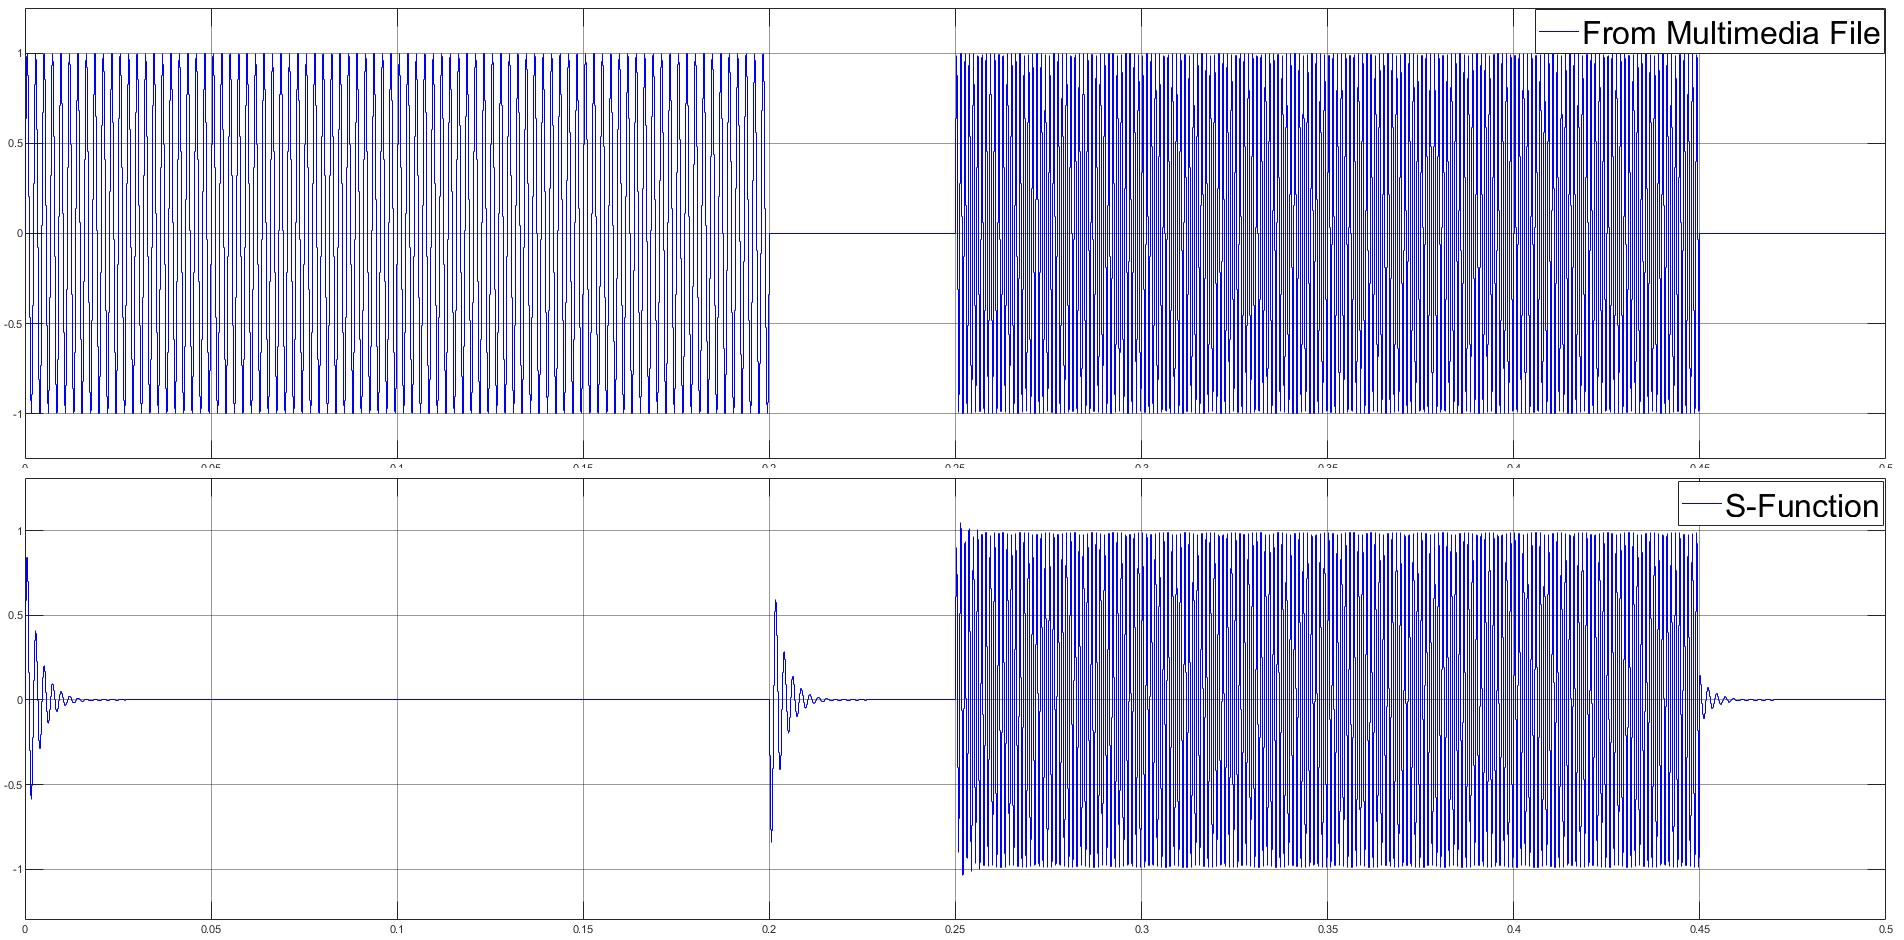
\includegraphics[scale = 0.2]{Figuras/p6_1- alternate_tones_bw100.jpg}
    \caption{Gráfica  en el tiempo de la señal de audio \textit{alternate\_tones\_16\_16.wav} antes y después de ser filtrada con ancho de banda de $100~Hz$}
    \label{alternate100}
\end{figure}



Se diseñan nuevos filtros Notch que realicen la misma tarea pero esta vez con un ancho de banda de $50~Hz$ y $200~Hz$ respectivamente, los resultados obtenidos se muestran en las figuras  \ref{bw50} y \ref{bw200}


\begin{figure}[H]
    \centering
    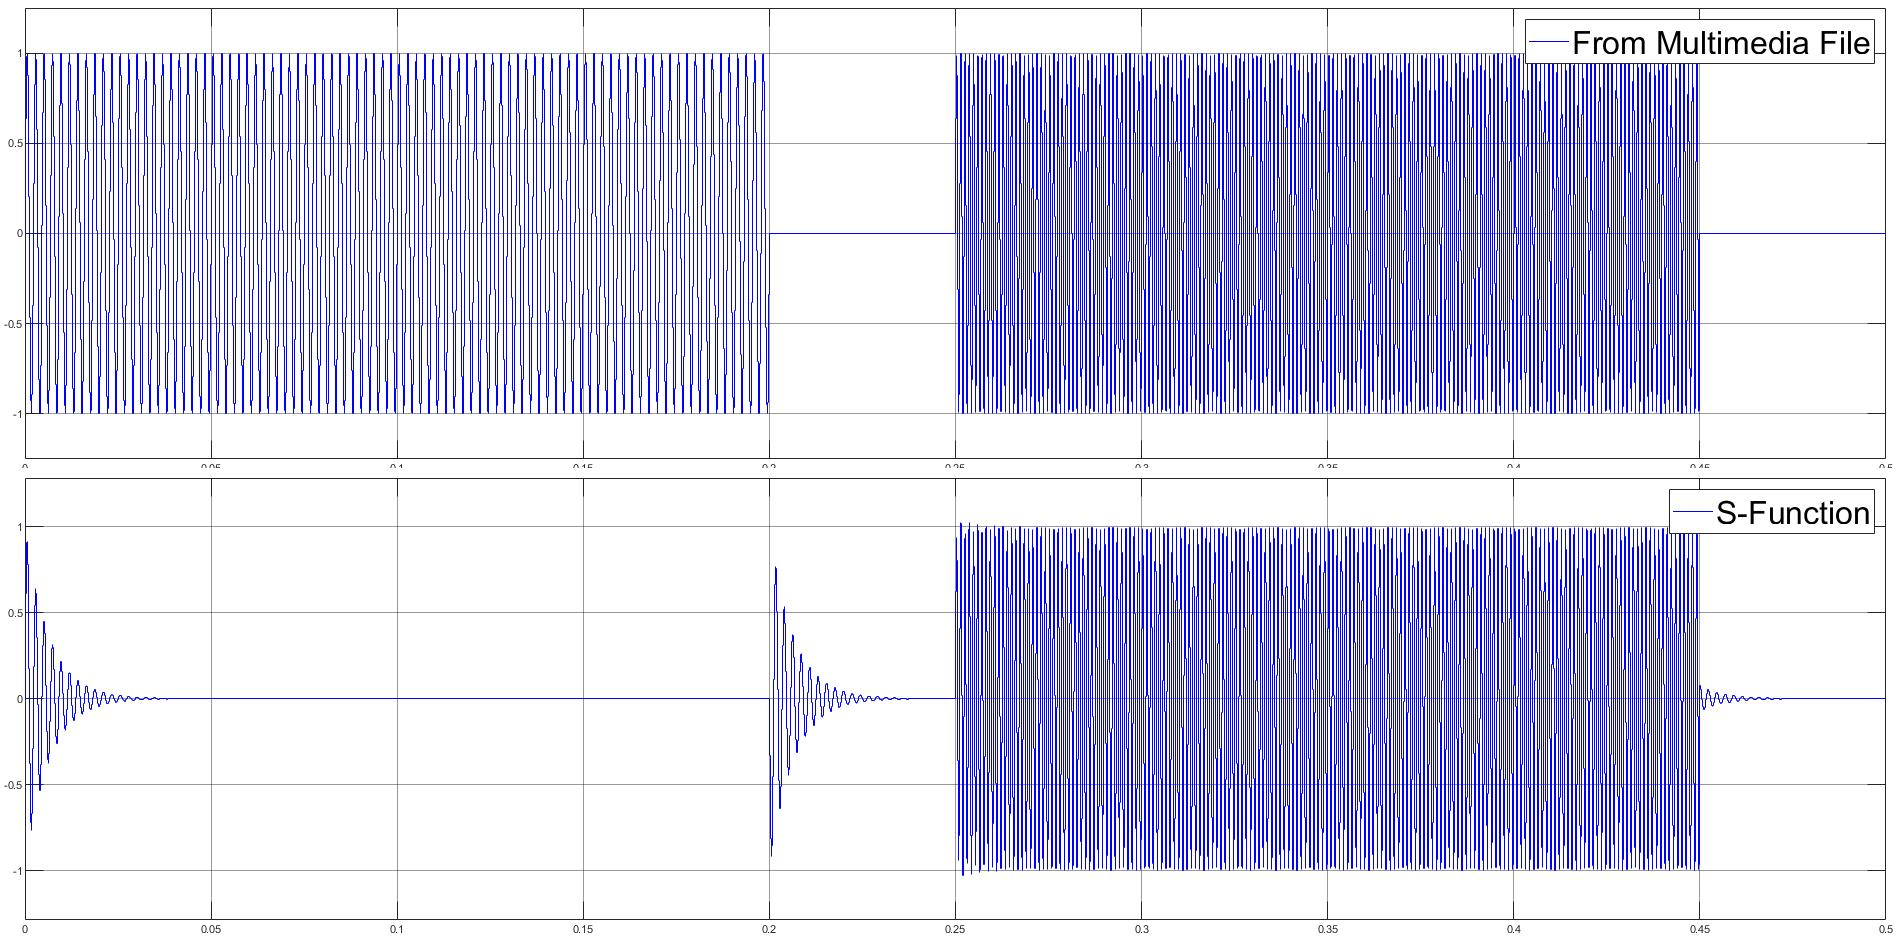
\includegraphics[scale = 0.2]{Figuras/p6_1- alternate_tones_bw50.jpg}
    \caption{Gráfica  en el tiempo en segundos de la señal de audio \textit{alternate\_tones\_16\_16.wav} antes y después de ser filtrada con ancho de banda de $50~Hz$}
    \label{bw50}
\end{figure}


\begin{figure}[H]
    \centering
    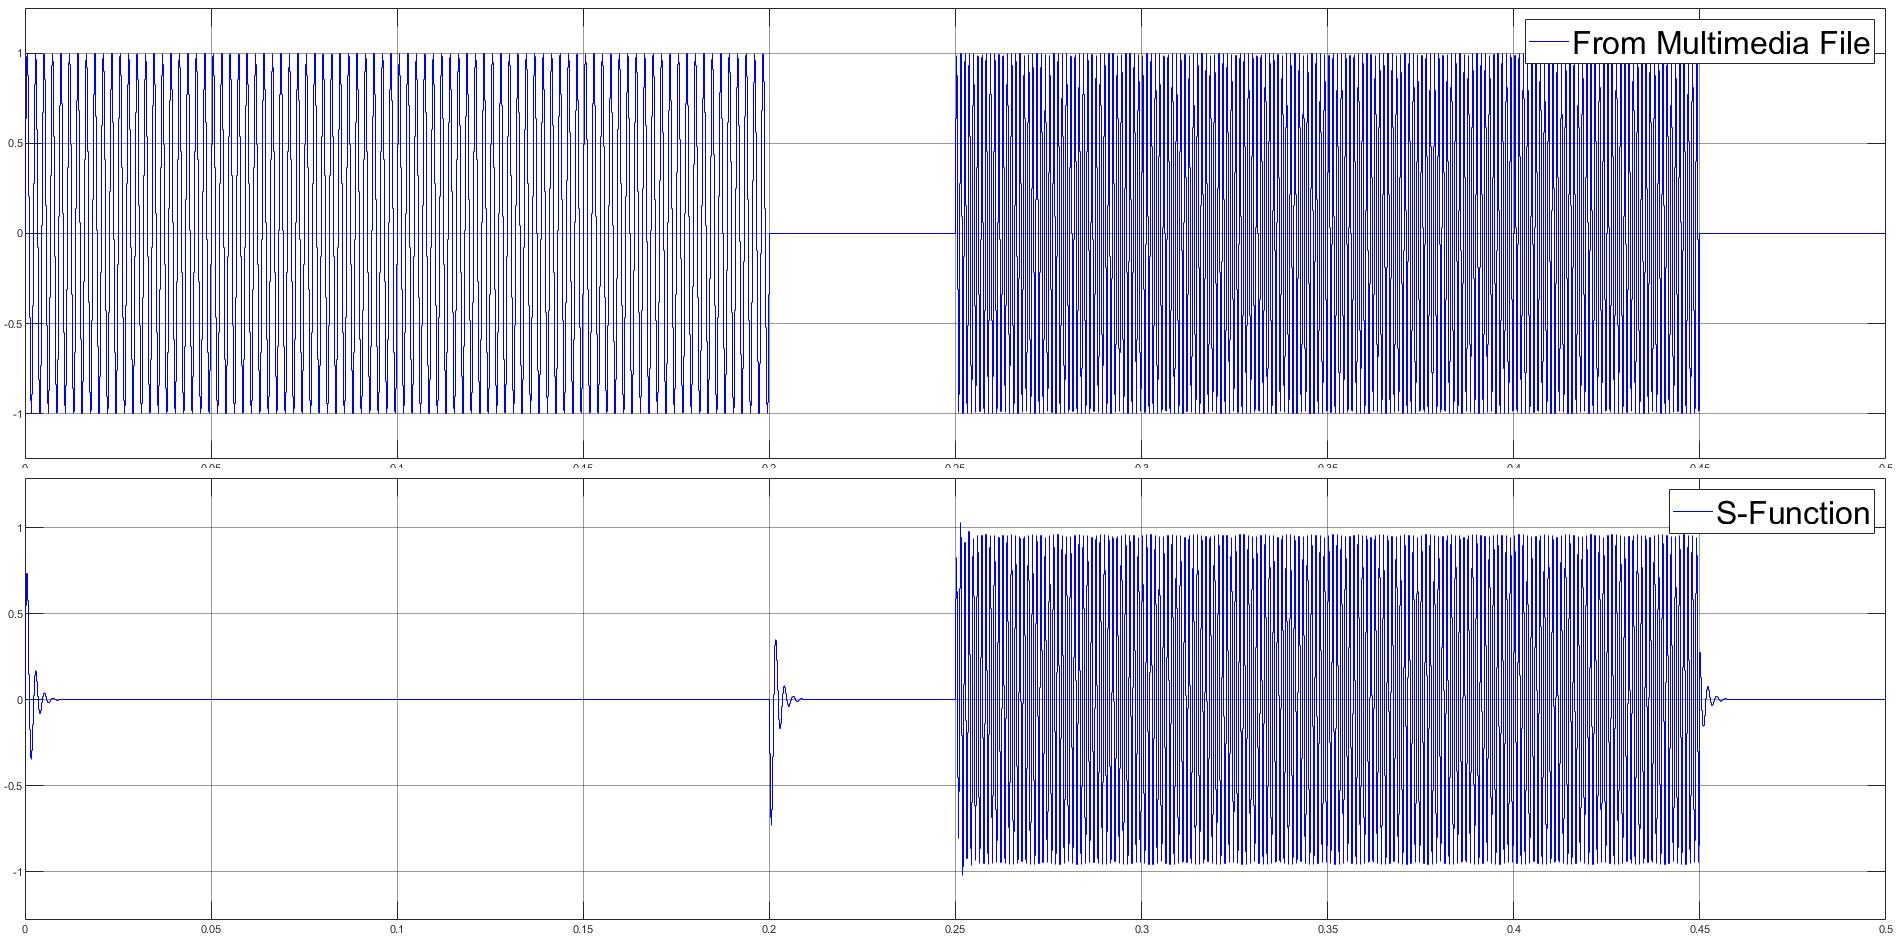
\includegraphics[scale = 0.2]{Figuras/p6_1- alternate_tones_bw200.jpg}
    \caption{Gráfica  en el tiempo en segundos de la señal de audio \textit{alternate\_tones\_16\_16.wav} antes y después de ser filtrada con ancho de banda de $200~Hz$}
    \label{bw200}
\end{figure}


Se puede observar como en todos los casos existe un transciente antes de que se realice efectivamente el filtrado, se concluir por las pruebas realizadas que dicho transciente tiene menor duración en la medida en que aumenta el ancho de banda del filtro. Esto se puede ver de mejor manera observando la respuesta a impulso de los tres filtros diseñados, las respuestas a impulso se encuentran en las figuras \ref{impbw50}, \ref{impbw100} y \ref{impbw200} para los anchos de banda de $50~Hz$, $100~Hz$ y $200~Hz$ respectivamente.

\begin{figure}[H]
    \centering
    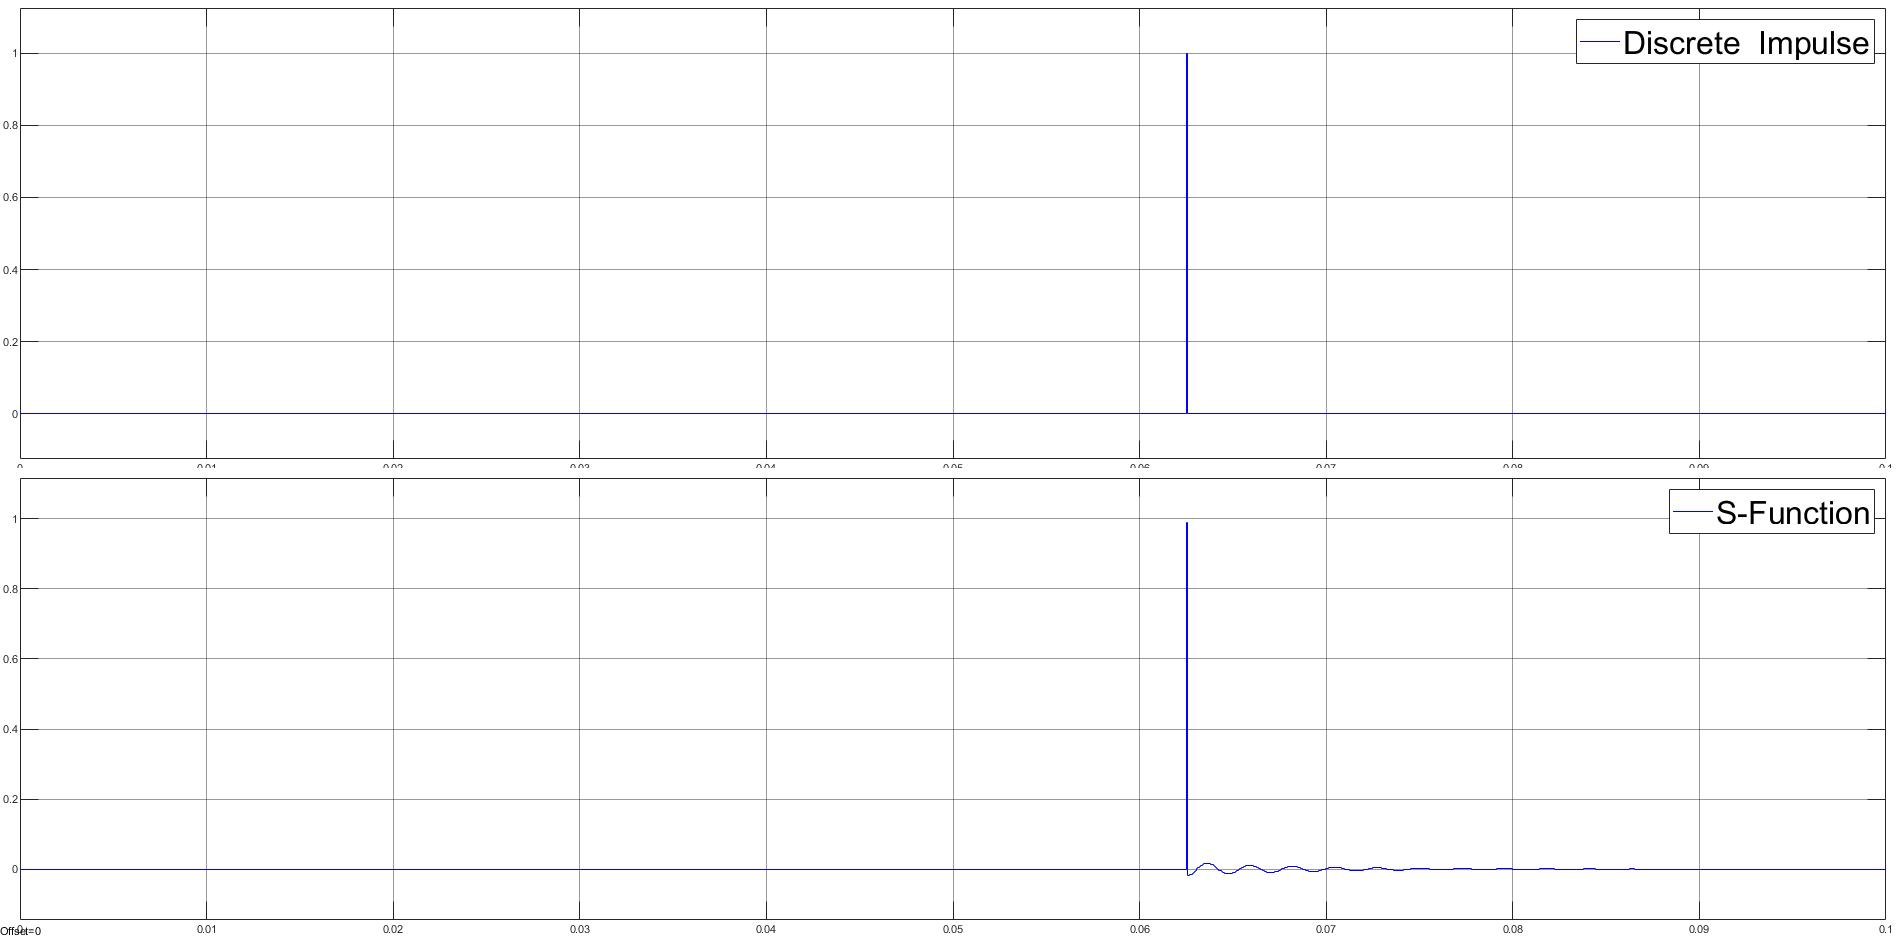
\includegraphics[scale = 0.2]{Figuras/p6_1-Impulse_50.jpg}
    \caption{Gráfica en el tiempo en segundos  de la respuesta impulso del filtro diseñado con ancho de banda de $50~Hz$.}
    \label{impbw50}
\end{figure}


\begin{figure}[H]
    \centering
    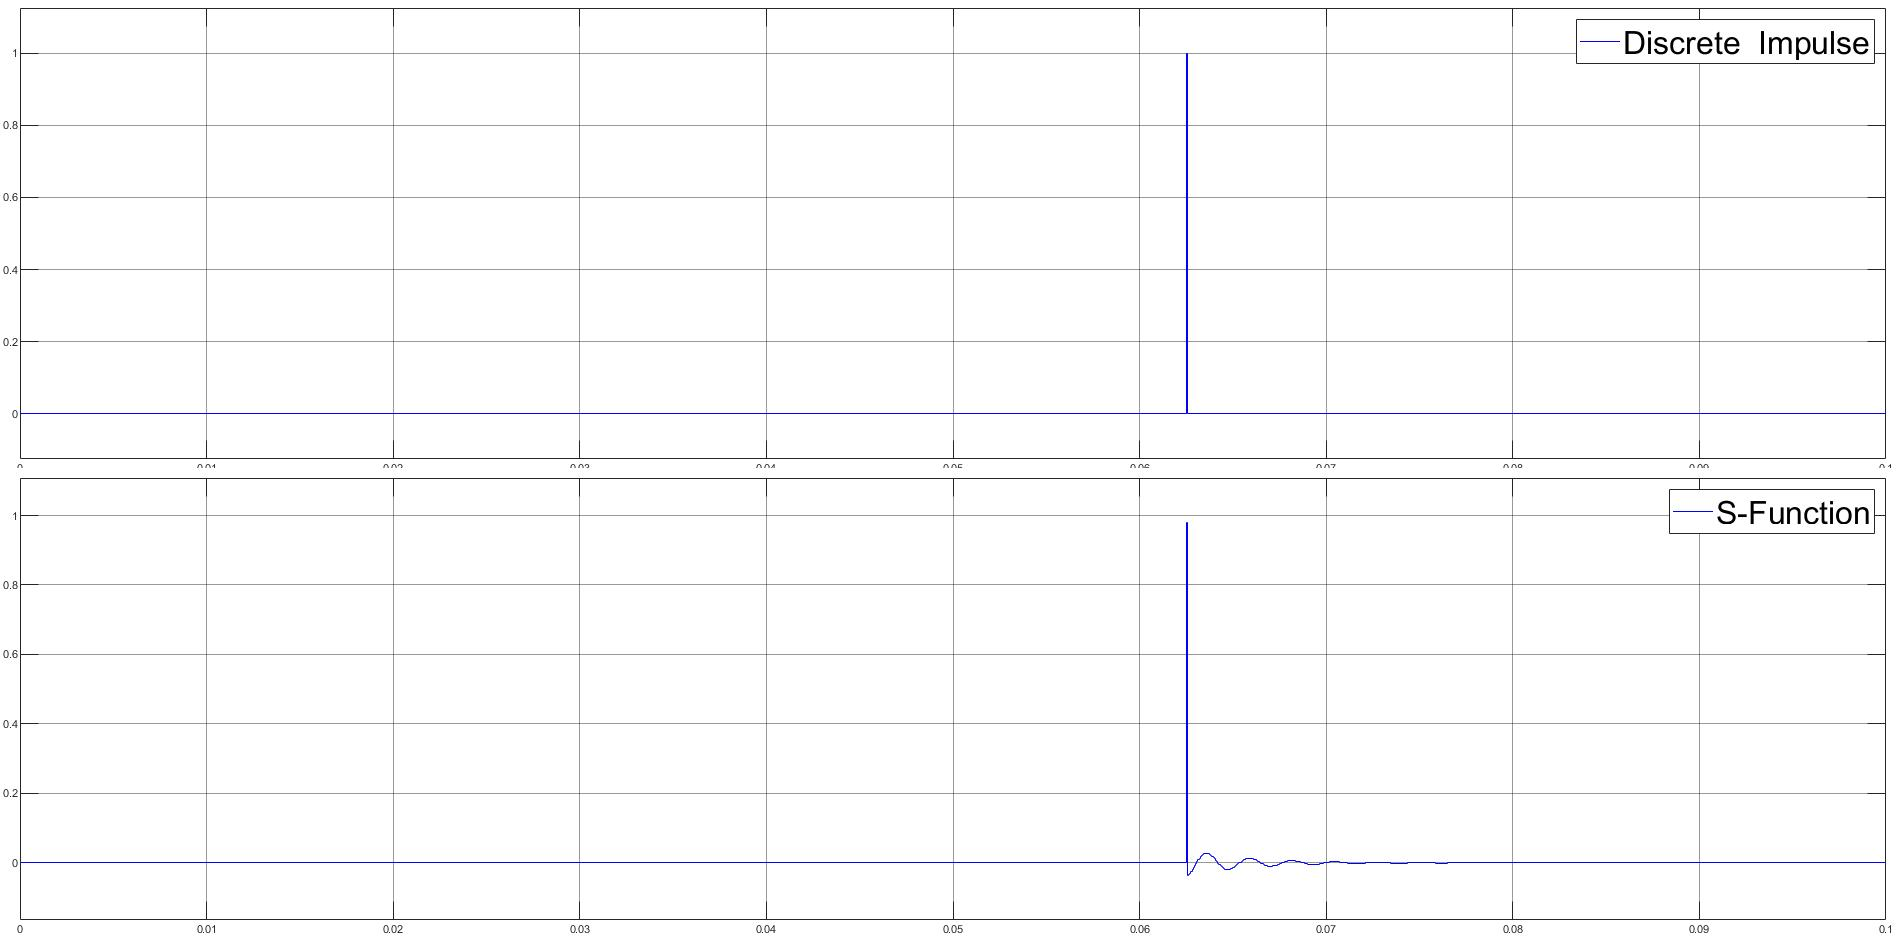
\includegraphics[scale = 0.2]{Figuras/p6_1-Impulse_100.jpg}
    \caption{Gráfica en el tiempo en segundos de la respuesta impulso del filtro diseñado con ancho de banda de $100~Hz$.}
    \label{impbw100}
\end{figure}

\begin{figure}[H]
    \centering
    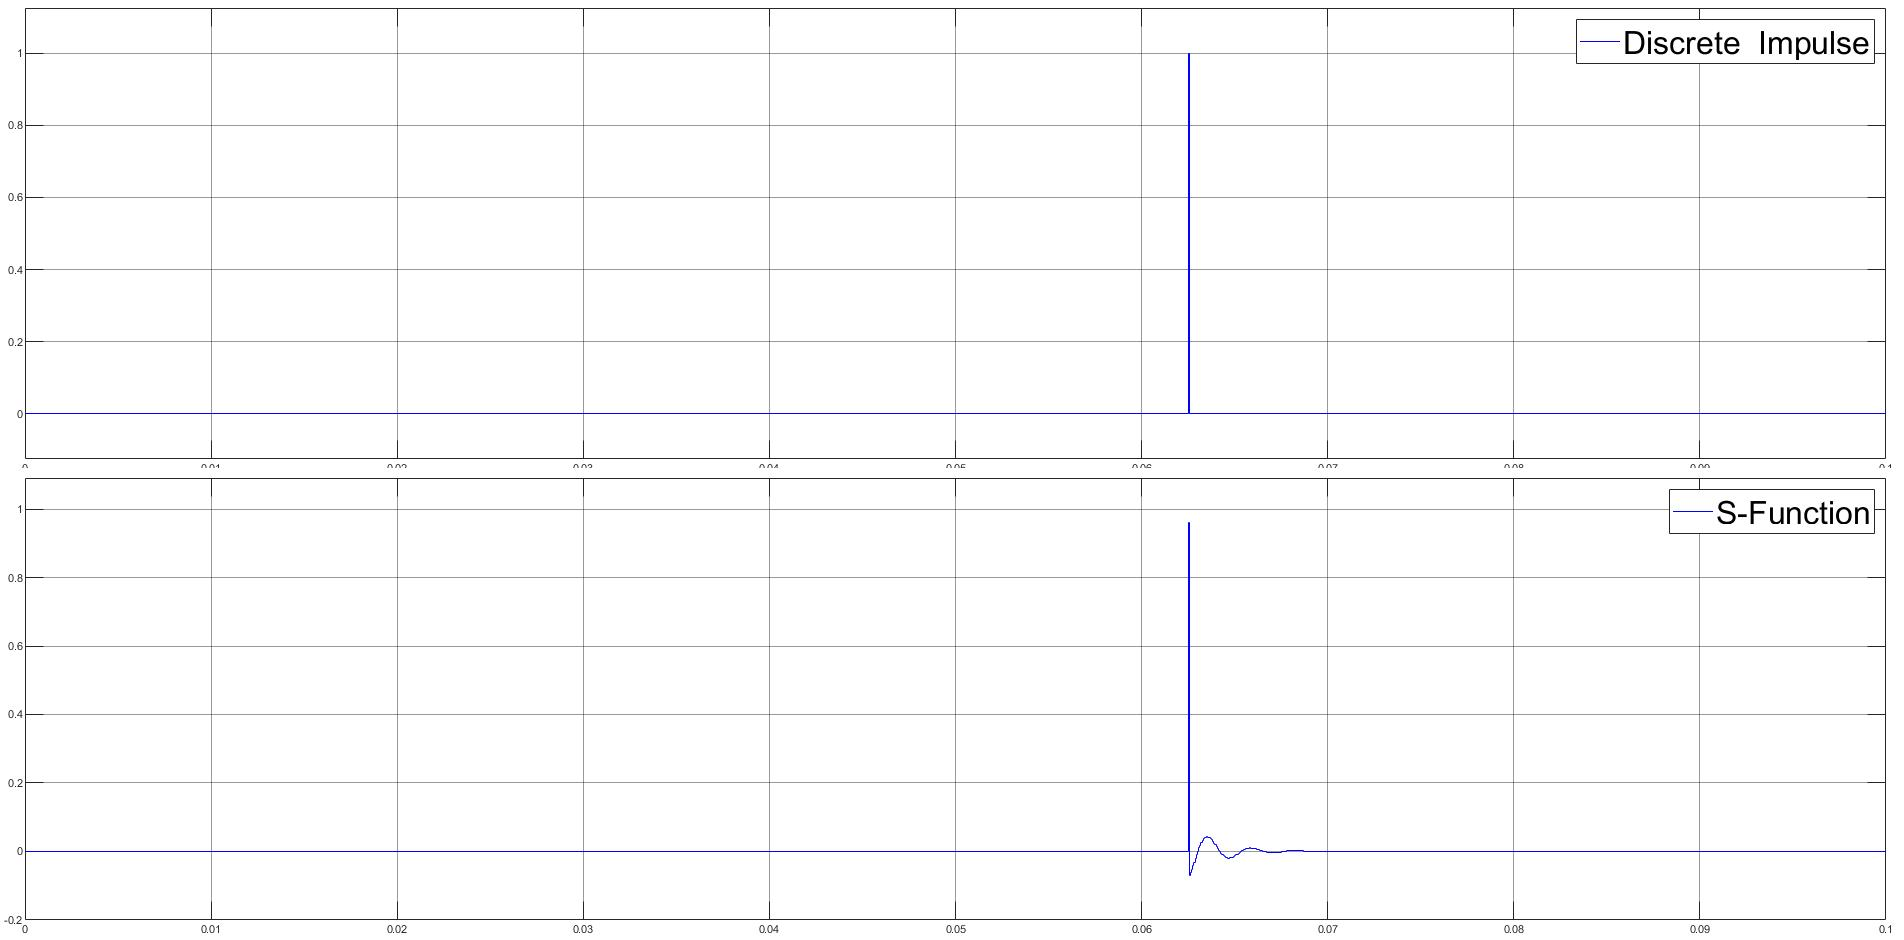
\includegraphics[scale = 0.2]{Figuras/p6_1-Impulse_200.jpg}
    \caption{Gráfica en el tiempo en segundos de la respuesta impulso del filtro diseñado con ancho de banda de $200~Hz$.}
    \label{impbw200}
\end{figure}


En las tres gráficas anteriores se puede comprobar lo antes mencionado sobre la relación inversa que existe entre la duración de la respuesta temporal del filtro con el ancho de banda permitido por este.

%Rodrigo
\item En esta sección se implementa filtro notch (elimina banda angosta) de segundo orden cuya frecuencia central pueda ser sintonizada en tiempo real. Para lo anterior se creó la función \texttt{filterInterface()} en C, la cual actualiza los parámetros del filtro, llama a la función \texttt{filterBiquad()} y actualiza la salida.

La primera parte de la sección de actualización de parámetros del filtro se muestra a continuación:\clearpage
\begin{lstlisting}[language = C]
void filterInterface(double input1, double input2,
                     double* output1) {

    //Calculo parámetros filtro
    double BW    = 2 * PI * 100 / 16000;    // (BW Norm)
    double theta = 2 * PI * input2 / 16000; // (wc Norm)

    double p[] = { cos(BW), -2, cos(BW) };
    double d1 = (-p[2] + sqrt(p[2] * p[2] - 4 * p[1] * p[3])) 
                / 2 * p[1];
    double d2 = (-p[2] - sqrt(p[2] * p[2] - 4 * p[1] * p[3])) 
                / 2 * p[1];

    double d;
    if (abs(d1) < abs(d2)) {
        d = d1;
    }
    else {
        d = d2;
    }
\end{lstlisting}
donde se utiliza la expresión de la solución de la ecuación cuadrática característica del filtro notch (\ref{p4_cuadratica}) y se extrae la extrae la solución que está dentro del círculo unitario por estabilidad.

La segunda parte de la sección de actualización de parámetros del filtro se muestra a continuación:
\begin{lstlisting}[language = C]
    //Actualizacion de parametros filtro
    static bqState_t Notch_variable = {
                      0,  // a1
                      0, // a2
                      0, //b0
                      0,//b1
                      0,  //b2

                      {0, 0, 0}, //Inputs buffer
                      {0, 0, 0} //Outputs buffer
    };

    (&Notch_variable)->bqA1 = -(1 + d) * cos(theta);
    (&Notch_variable)->bqA2 = d;
    (&Notch_variable)->bqB0 = (1 + d) / 2;
    (&Notch_variable)->bqB1 = (1 + d) / 2 * -2 * cos(theta);
    (&Notch_variable)->bqB2 = (1 + d) / 2;

\end{lstlisting}
donde se utiliza la función de transferencia dependiente de $d$ (\ref{p6_Transfer}) para obtener los coeficientes $a_i$ y $b_i$.

Finalmente se llama a la función \texttt{filterBiquad()} como se muestra a continuación con el filtro ya actualizado.
\begin{lstlisting}[language = C]
//Llamado a funcion de filtrado y seteo de salida
    *output1 = filterBiquad(&Notch_variable, input1);
}
\end{lstlisting}
Ya con \texttt{filterInterface()} implementada, se genera la función para crear la s-Function:

\begin{lstlisting}[language = C]
extern double notch(double data1, double data2)
{
    double output;
    filterInterface(data1, data2, &output);
    return output;
}
\end{lstlisting}

Posteriormente se creó un diagrama en simulink para probar la s-Function. Dicho diagrama se muestra en la figura \ref{fig:p6_2_simulink}. Aquí se ocupo el bloque \textit{Repeating Sequence Interpolated} para generar la señal de control de frecuencia central, donde la señal se mantiene en 440 Hz el primer segundo, luego aumenta a razón constante hasta el segundo 3 donde se queda en 880 Hz hasta los 3.9 s (donde se termina la simulación). 
\begin{figure}[H]
    \centering
    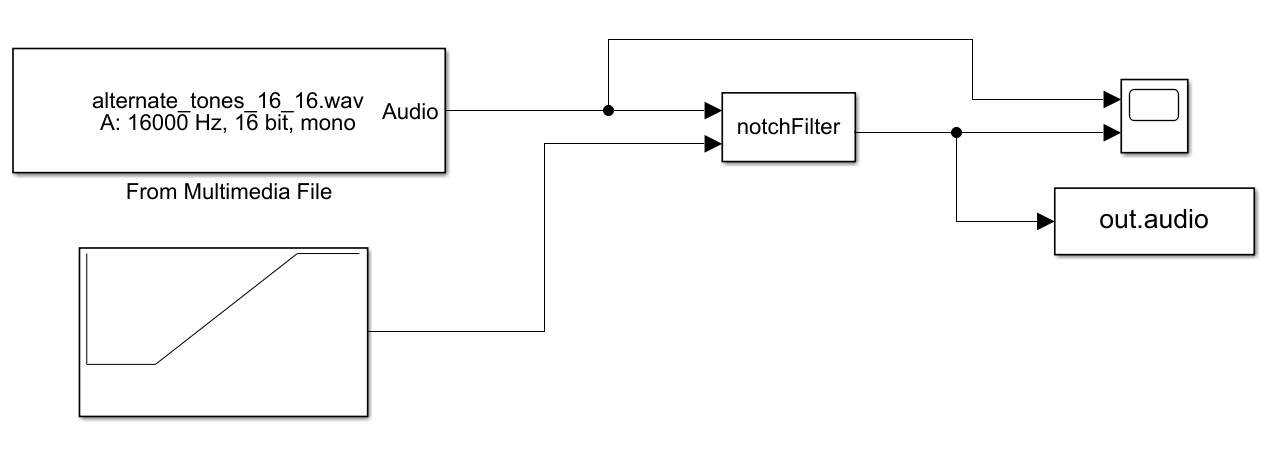
\includegraphics[width = .8\linewidth]{Figuras/p6_2_simulink.png}
    \caption{Diagrama en simulink para el testeo de la s-Function de notch ajustable}
    \label{fig:p6_2_simulink}
\end{figure}
 
 La señal de  audio a filtrar(\textit{alternate\_tones\_16\_16.wav}) y la filtrada se muestra en la figura \ref{fig:p6_2_scope}. Se observa que durante el primer segundo se filtra la primera señal en 440 Hz, que a partir del segundo 3 se filtra la segunda en 880 Hz y que existe una transición entre el segundo 1 y 3. Resulta interesante destacar que el filtro también afecta la amplitud de la señal que se desea dejar pasar. 
 
 \begin{figure}[H]
    \centering
    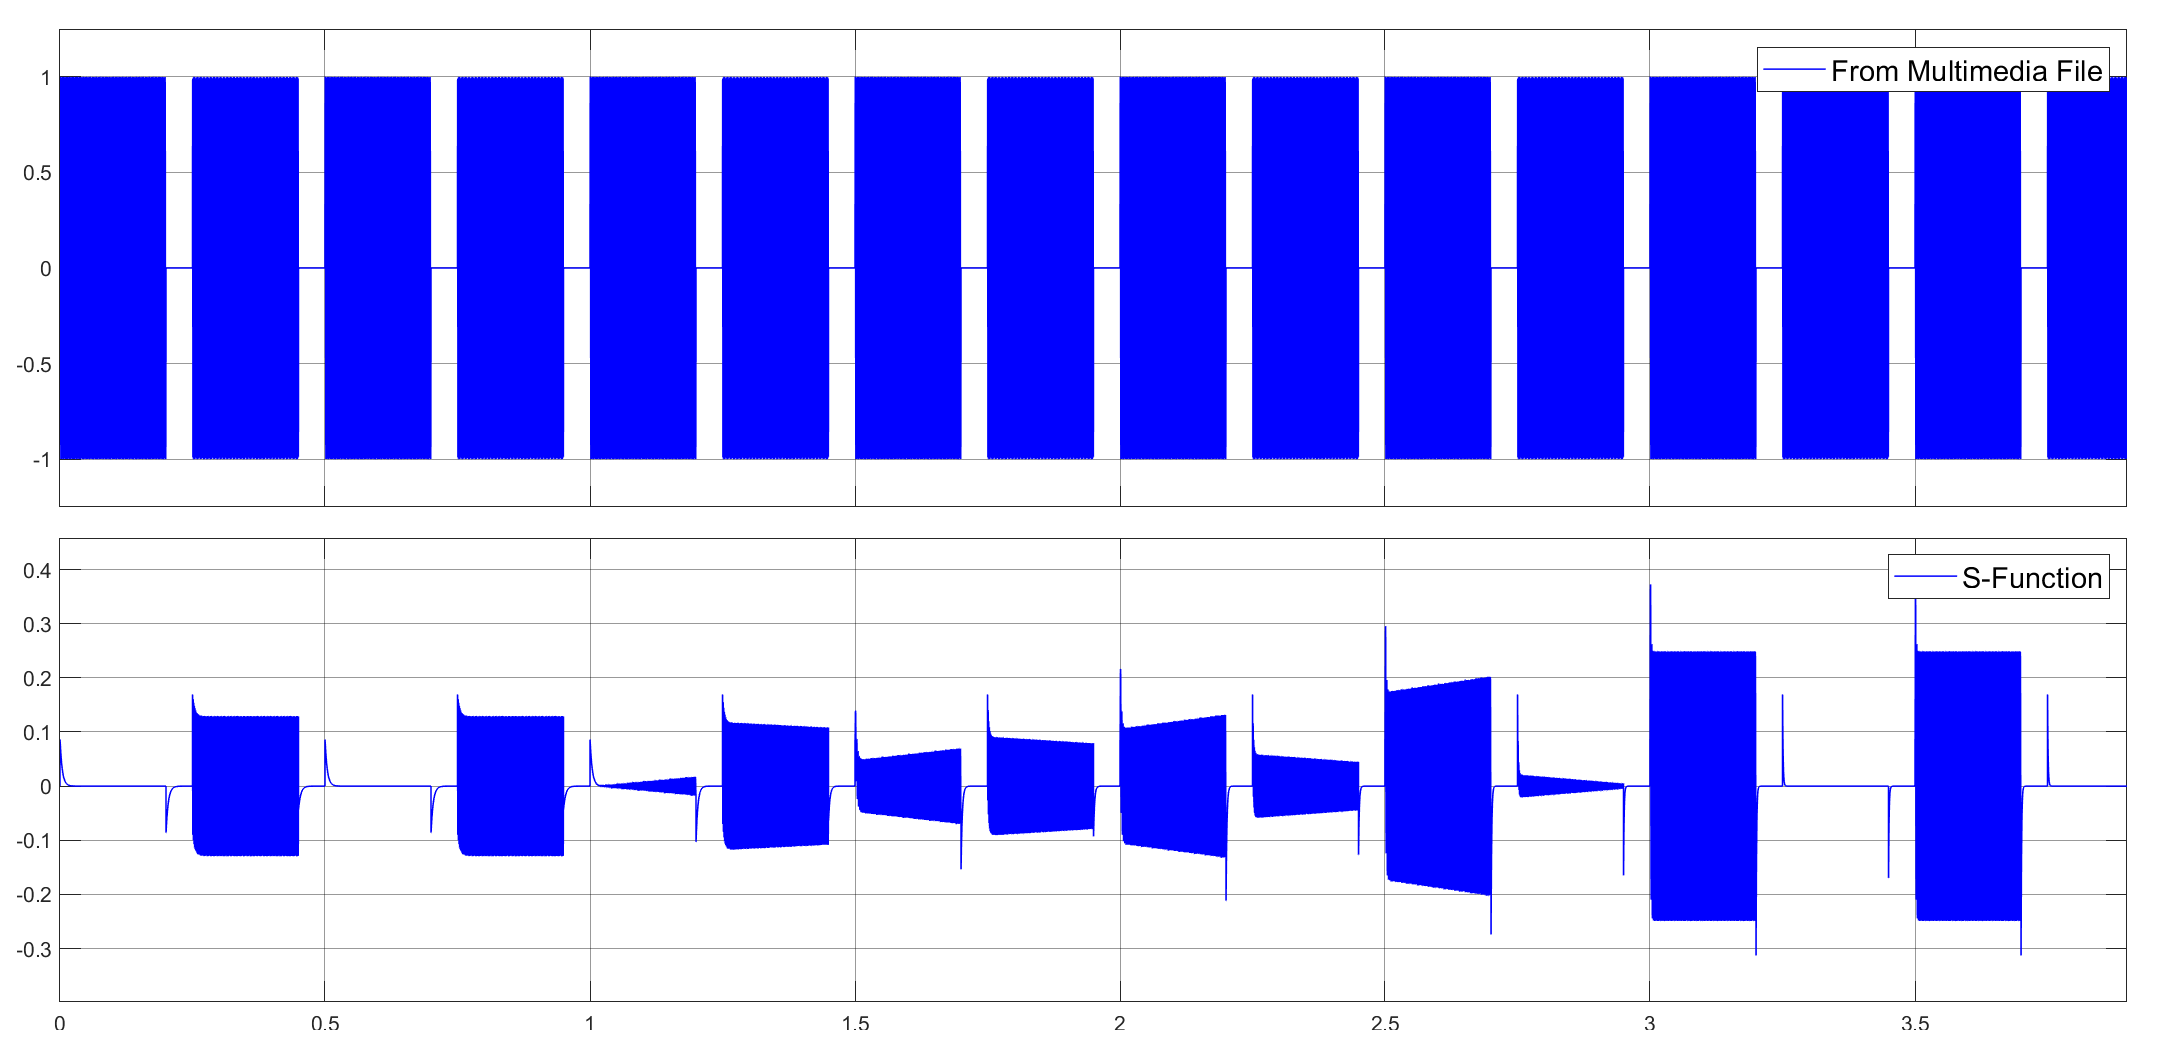
\includegraphics[width = .8\linewidth]{Figuras/p6_2_scope.eps}
    \caption{Amplitud [-] vs tiempo [s] de señal de entrada al filtro notch ajustable (arriba) y señal resultante del filtrado (abajo).}
    \label{fig:p6_2_scope}
\end{figure}

La señal de salida se guarda en el archivo de audio \texttt{p6\_2\_alternate\_audio\_16.wav} el cual se adjunta en la entrega. Auditívamente se aprecia correcto funcionamiento del esquema (no percepción de la frecuencia baja al inicio y solo percepción de la frecuencia alta al final).

%Richi
\item  Se diseñan 7 filtros pasa banda angosta para poder identificar tonos dtmf presentes en el archivo de audio \textit{dtmf\_secuence.wav}. Para esto se deben escoger los coeficientes $a_k$ y $b_k$ asociados a la función de transferencia de la forma de un filtro Biquad que se ha estado utilizando, de manera que cada filtro permita pasar una des las frecuencias de los tonos dtmf es decir

$$BPF0: ~~ 696~Hz $$
$$BPF1: ~~ 770~Hz  $$
$$BPF2: ~~ 852~Hz  $$
$$BPF3: ~~ 941~Hz  $$ 
$$BPF4: ~~ 1209~Hz  $$ 
$$BPF5: ~~ 1336~Hz  $$
$$BPF6: ~~ 1447~Hz  $$


Se desarrolló un script en MATLAB que permite obtener los coeficientes necesarios para filtrar cada una de las frecuencias dado un ancho de banda y  una frecuencia de muestreo. Se escogió un ancho de banda de $20~Hz$, ya que es un valor que permite aislar completamente cada frecuencia deseada asegurando que no aparezcan componentes de otras frecuencias que no le corresponden al filtro asociado. Se hicieron pruebas con anchos de banda mas holgados considerando las consecuencias en la respuesta temporal que este parámetro implica (un ancho de banda mayor genera una respuesta transciente menor) pero no se logró filtrar de manera precisa la frecuencias de interés.

El cuadro \ref{coeficientes} muestra los coeficientes $a_k$ y $b_k$ correspondientes a cada filtro asociado a una frecuencia específica


 
 \begin{table}[H]
        \centering
        \begin{tabular}{|c|c|c|c|c|c|}
        \hline
         Frecuencia [Hz]   & a_1 & a_2 & b_0 & b_1 & b_2\\
         \hline
         697  &  -1.91801  & 0.99217 &  0.00391             &      0&  -0.00391 \\
         \hline
         770  & -1.90179 &  0.99217 & 0.00391          &        0  &-0.00391	 \\
         \hline
         852 &   -1.88170 &  0.99217 & 0.00391       &          0 & -0.00391\\
         \hline
        
         941  & -1.85769 &  0.99217 &  0.00391      &          0 & -0.00391\\
         \hline
        
        1209  &  -1.77183 &  0.99217&	  0.00391         &      0 & -0.00391\\
         \hline
        
         1336  & 	-1.72423 &  0.99217  & 0.00391     &             0 & -0.00391\\
         \hline
         
        1447  &  -1.66636 &  0.99217 &  0.00391     &             0&  -0.00391	\\
         \hline

        \end{tabular}
        \caption{Cuadro resumen de los coeficientes de $a_k$ y $b_k$ de los filtros asociados a cada frecuencia dtmf.}
        \label{coeficientes}
    \end{table}
    
    
    Para implementar los filtros se creó para cada uno  estructura del tipo \texttt{bqState\_t} como la que se ha estado usando hasta el momento con los coeficientes asociados a cada uno de los mismos, se reutiliza la función \texttt{filterBiquad} ya implementada y se desarrolla la función \texttt{decodeDtmf} que llama a las funciones entregadas como recurso para el laboraorio para poder ejecutar la decodificación que se busca. El código de la función \texttt{decodeDtmf} es el siguiente
    
    \begin{lstlisting}[language = C]
extern  void decodeDtmf(double input1, int32_t *output1){
  gDtmfTones[0] = filterBiquad(&BPF0,input1);
  gDtmfTones[1] = filterBiquad(&BPF1,input1);
  gDtmfTones[2] = filterBiquad(&BPF2,input1);
  gDtmfTones[3] = filterBiquad(&BPF3,input1);
  gDtmfTones[4] = filterBiquad(&BPF4,input1);
  gDtmfTones[5] = filterBiquad(&BPF5,input1);
  gDtmfTones[6] = filterBiquad(&BPF6,input1);

  *output1 =   dtmfDetection(gDtmfTones);
}
    \end{lstlisting}


Al simular el filtrado de la señal de audio \textit{dtmf\_secuence.wav} con los filtros implementados se obtiene la gráfica que se muestra en la figura \ref{dtmf}

\begin{figure}[H]
    \centering
    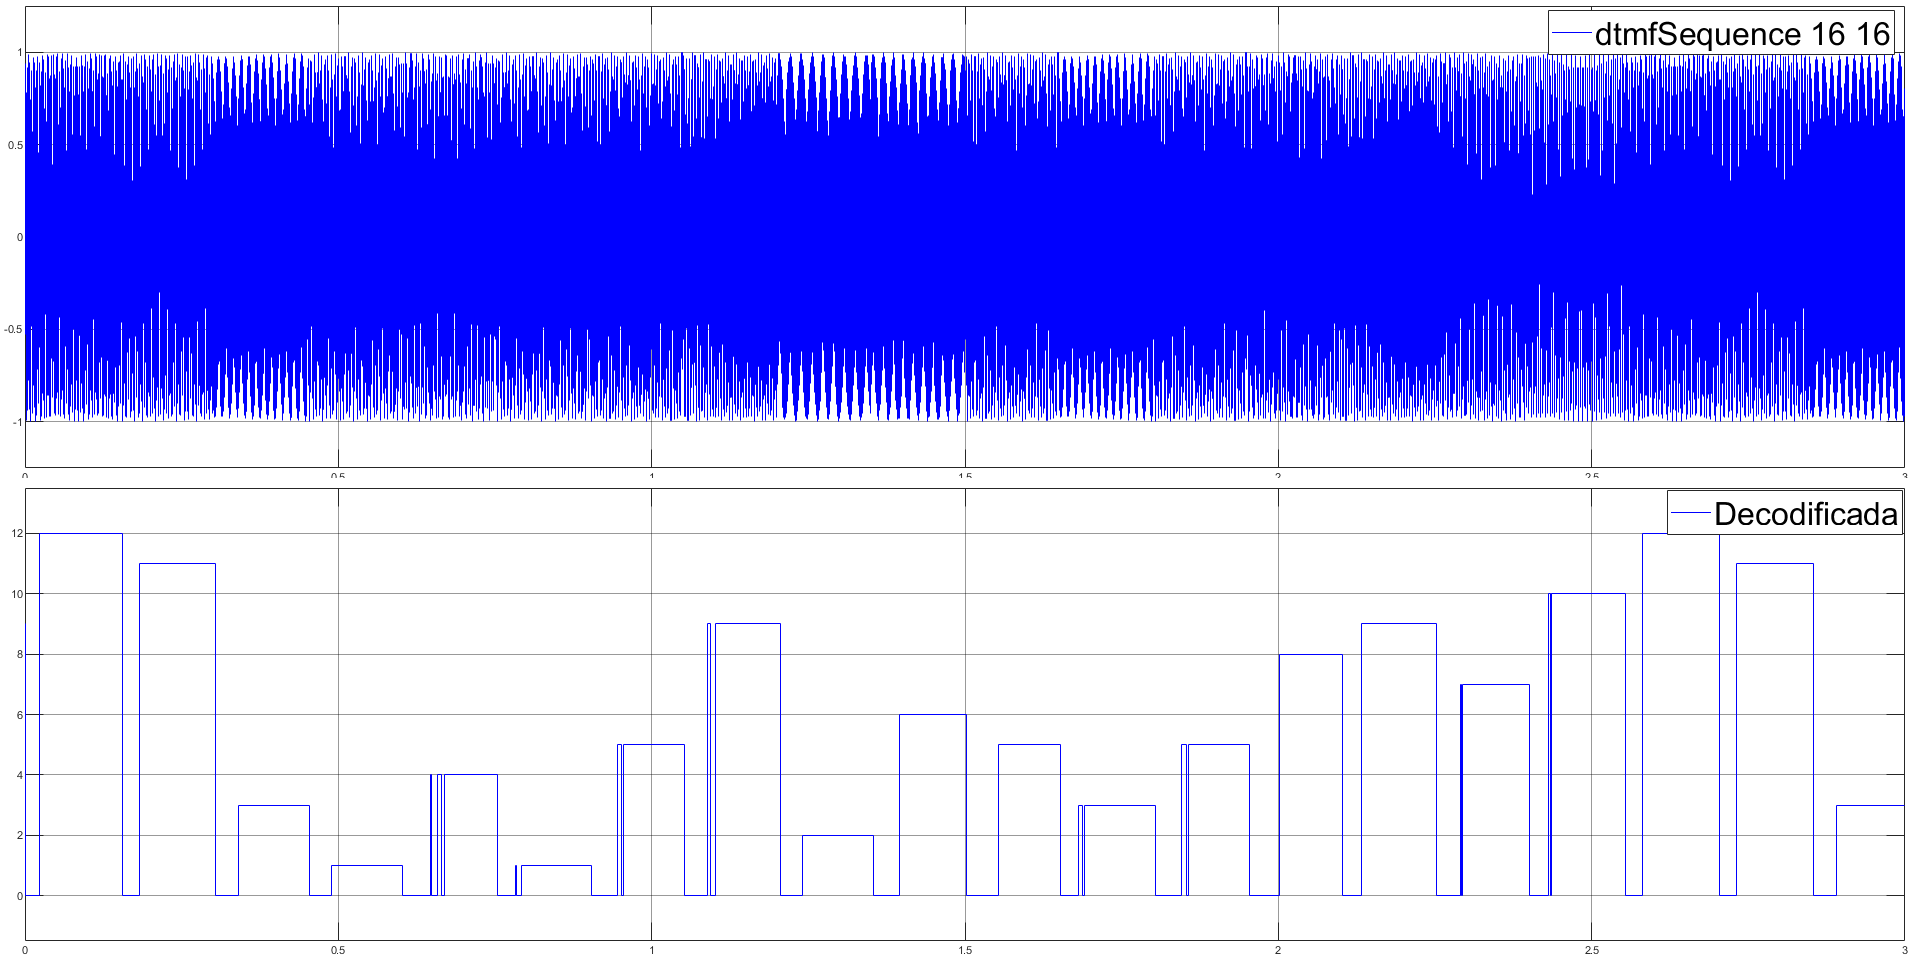
\includegraphics[scale = 0.3]{Figuras/p6_3-Dtmf.png}
    \caption{Gráfica en el tiempo en segundos de la simulación de filtrado de la señal de audio \textit{dtmf\_secuence.wav} con 7 filtros BPF  en paralelo.}
    \label{dtmf}
\end{figure}


La gráfica superior muestra el archivo de audio en el tiempo  y la gráfica inferior muestra el resultado obtenido luego de filtrar la señal, donde se puede reconocer  la secuencia dtmf era \texttt{\#-*-3-1-4-1-5-9-2-6-5... - \#}.

\end{enumerate}



\newpage
\section{Fe de erratas}
\subsection{Etiquetas de imagenes con errores}
\begin{itemize}
    \item Figura 2 etiqueta en el eje x: \textbf{\textit{rad/s}}. Debería ser eje x: \textbf{\textit{rad/muestra}}
    \item Figura 3 etiqueta en el eje x: \textbf{\textit{rad/s}}. Debería ser eje x: \textbf{\textit{rad/muestra}}
    \item Figura 6 etiqueta en el eje x: \textbf{\textit{rad/s}}. Debería ser eje x: \textbf{\textit{rad/muestra}}
    \item Figura 7 etiqueta en el eje x: \textbf{\textit{rad/s}}. Debería ser eje x: \textbf{\textit{rad/muestra}}
    \item Figura 8 etiqueta en el eje x: \textbf{\textit{rad/s}}. Debería ser eje x: \textbf{\textit{rad/muestra}}
    \item Figura 9 etiqueta en el eje x: \textbf{\textit{rad/s}}. Debería ser eje x: \textbf{\textit{rad/muestra}}
    \item Figura 10 etiqueta en el eje x: \textbf{\textit{rad/s}}. Debería ser eje x: \textbf{\textit{rad/muestra}}
    \item Figura 12 etiqueta en el eje x: \textbf{\textit{rad/s}}. Debería ser eje x: \textbf{\textit{rad/muestra}}
    \item Figura 13 etiqueta en el eje x: \textbf{\textit{rad/s}}. Debería ser eje x: \textbf{\textit{rad/muestra}}
    \item Figura 14 etiqueta en el eje x: \textbf{\textit{rad/s}}. Debería ser eje x: \textbf{\textit{rad/muestra}}
     
\end{itemize}











\end{document}

